\documentclass[12pt, a4paper]{article}

\usepackage{graphicx}
\usepackage{microtype}
\usepackage{amsmath}
\usepackage[hidelinks]{hyperref}
\usepackage[table]{xcolor}
\usepackage{geometry}
\usepackage{fancyhdr}
\usepackage[inkscapelatex=false]{svg}
\usepackage{extsizes}
\usepackage{fontspec}
\usepackage{float}
\usepackage{csvsimple}
\usepackage{array}
\usepackage{enumitem}
\usepackage[none]{hyphenat}
\usepackage{quoting}
\usepackage{tikz}
\usepackage{contour}
\usepackage{tabularx}
\usepackage{relsize}

\pdfstringdefDisableCommands{\def\enspace{\space}\def\smaller{}\def\larger{}}

\setmainfont{Barlow}[
    Path=./fonts/,
    Extension = .ttf,
    UprightFont = *-Medium,
    BoldFont = *-SemiBold,
    ItalicFont = *-MediumItalic,
    BoldItalicFont = *-SemiBoldItalic,
]

\newfontfamily\ibmplex{IBMPlexMono}[
    Path=./fonts/,
    Extension = .ttf,
    UprightFont = *-Medium,
    BoldFont = *-SemiBold,
    ItalicFont = *-MediumItalic,
    BoldItalicFont = *-SemiBoldItalic,
]

\geometry{
    a4paper,
    left=30mm,
    right=30mm,
    top=30mm,
    bottom=30mm,
}

\renewcommand{\subsectionautorefname}{see}

\parindent=0pt
\setlength{\parskip}{6pt}

\tolerance=1
\emergencystretch=\maxdimen
\hyphenpenalty=10000
\hbadness=10000

\quotingsetup{vskip=4pt}

\setlength{\headheight}{18pt}
\pagestyle{fancy}
\rhead{
    \includesvg[height=4.3mm]{svg/protorack.svg}
    \vspace{0.1mm}
}
\lhead{
    \textit{spark} inducer
    \hspace{1mm} - \hspace{1mm}
    ASSEMBLY MANUAL \scriptsize (Rev.3)
    \normalsize \vspace{0.75mm}
}
\lfoot{\ibmplex \scriptsize CERN-OHL-W-2.0+}
\rfoot{\scriptsize \textit{designed by Max Schlecht}}

\newcommand{\drawgrid}{
    \draw[help lines, red, xstep=0.1, ystep=0.1] (0,0) grid (1,1);
}

\newcommand{\drawrect}[2]{
    \draw[black, line width=2pt, rounded corners=3] (#1) rectangle (#2);
    \draw[white, line width=1pt, rounded corners=3] (#1) rectangle (#2);
}
\newcommand{\drawtext}[2]{
    \node[white] at (#1) {\contourlength{.075em}\contour{black}{#2}};
}

\newcommand{\checkbox}[1]{\CheckBox[backgroundcolor=0.86 0.828 0.71, name=#1]{}}

\begin{document}

\thispagestyle{empty}
\begin{center}
    \begin{minipage}{0.9\linewidth}
        \centering
        \vspace{4cm}
        {
            \Large
            \textit{spark} inducer \hspace{0.2em} - \hspace{0.2em} ASSEMBLY MANUAL
            \hspace{0.1em} \normalsize (Rev.3)
            \par
        }
        \vspace{1cm}
        \includesvg[width=\linewidth]{svg/spark_inducer.svg}\par
        \vspace{2cm}
        {\Large Designed by Max Schlecht\par}
        \vspace{0.5cm}
        {\large Licensed under \ibmplex CERN-OHL-W-2.0+ \par}
        \vspace{6cm}
        {\includesvg[height=4.3mm]{svg/protorack.svg} \hfill \large 2023}
    \end{minipage}
\end{center}
\clearpage

\section*{Introduction}

The \textit{spark} inducer is a development kit for prototyping audio circuits specially
designed for creating eurorack modules. It can be used to test your ideas in an isolated
environment (like you would do when breadboarding normally) but with the added benefit of easily
connecting to other eurorack compatible devices.

It can also be mounted in a standard eurorack enclosure, so you can quickly test how your
creation will perform in an actual patch. Permanent rack installation is also possible, but
additional precautions must be taken (\autoref{ssec:gluing}).

\vspace{2mm}

It features:
\begin{itemize}[topsep=2pt]
    \item 2x 830 point breadboards (BB830/MB-102 type)
    \item 6x general purpose connections (inputs or outputs) and 2x buffered outputs
    \item 4x arbitrary value potentiometers (the kit comes with $100k\Omega$ ones)
    \item preconnected analog power rails, digital +5V power (from the +5V bus)
    \item up to 4x selectable voltage references (positive and negative)
    \item power switch, status LEDs and resettable fuses on all power rails 
    \item being powered from a standard 16pin eurorack power connector
\end{itemize}

\vspace{3mm}

This DIY kit is perfect for intermediate builders who already know how to do basic through-hole
soldering but want to dip their feet into SMD soldering, as it mainly consists of relatively
easy to solder 0805 and 1206-sized passive components, some SOIC packages and a bunch of 2.54mm
headers.

{
    \color{red}
    \subsubsection*{Warning:}
    \vspace{-3mm}
    \textbf{%
        Even if you are an experienced builder, make sure to follow the build steps in the right
        order when building this kit. Some sections are very dense and will be almost impossible
        to assemble, if you do them in the wrong order.
    }
    \vspace{5mm}
}

\pagebreak

\section*{Required Tools}

\begin{itemize}
    \item Tweezers
    \item Side Cutters
    \item 1.5mm hex key
    \item Lead-Free Solder
    \\ {\small We use Stannol Kristall 611 (Sn96.5Ag3Cu0.5, 0.7mm) at 380°C.}
    \item Soldering Iron
    \\ {\small Temperature control is nice, but not strictly required.}
    \item Basic Multimeter
    \\ {\small Anything cheap that can measure Voltage and Continuity will do.}
    \item Eye Protection
\end{itemize}

\begin{figure}[H]
    \centering
    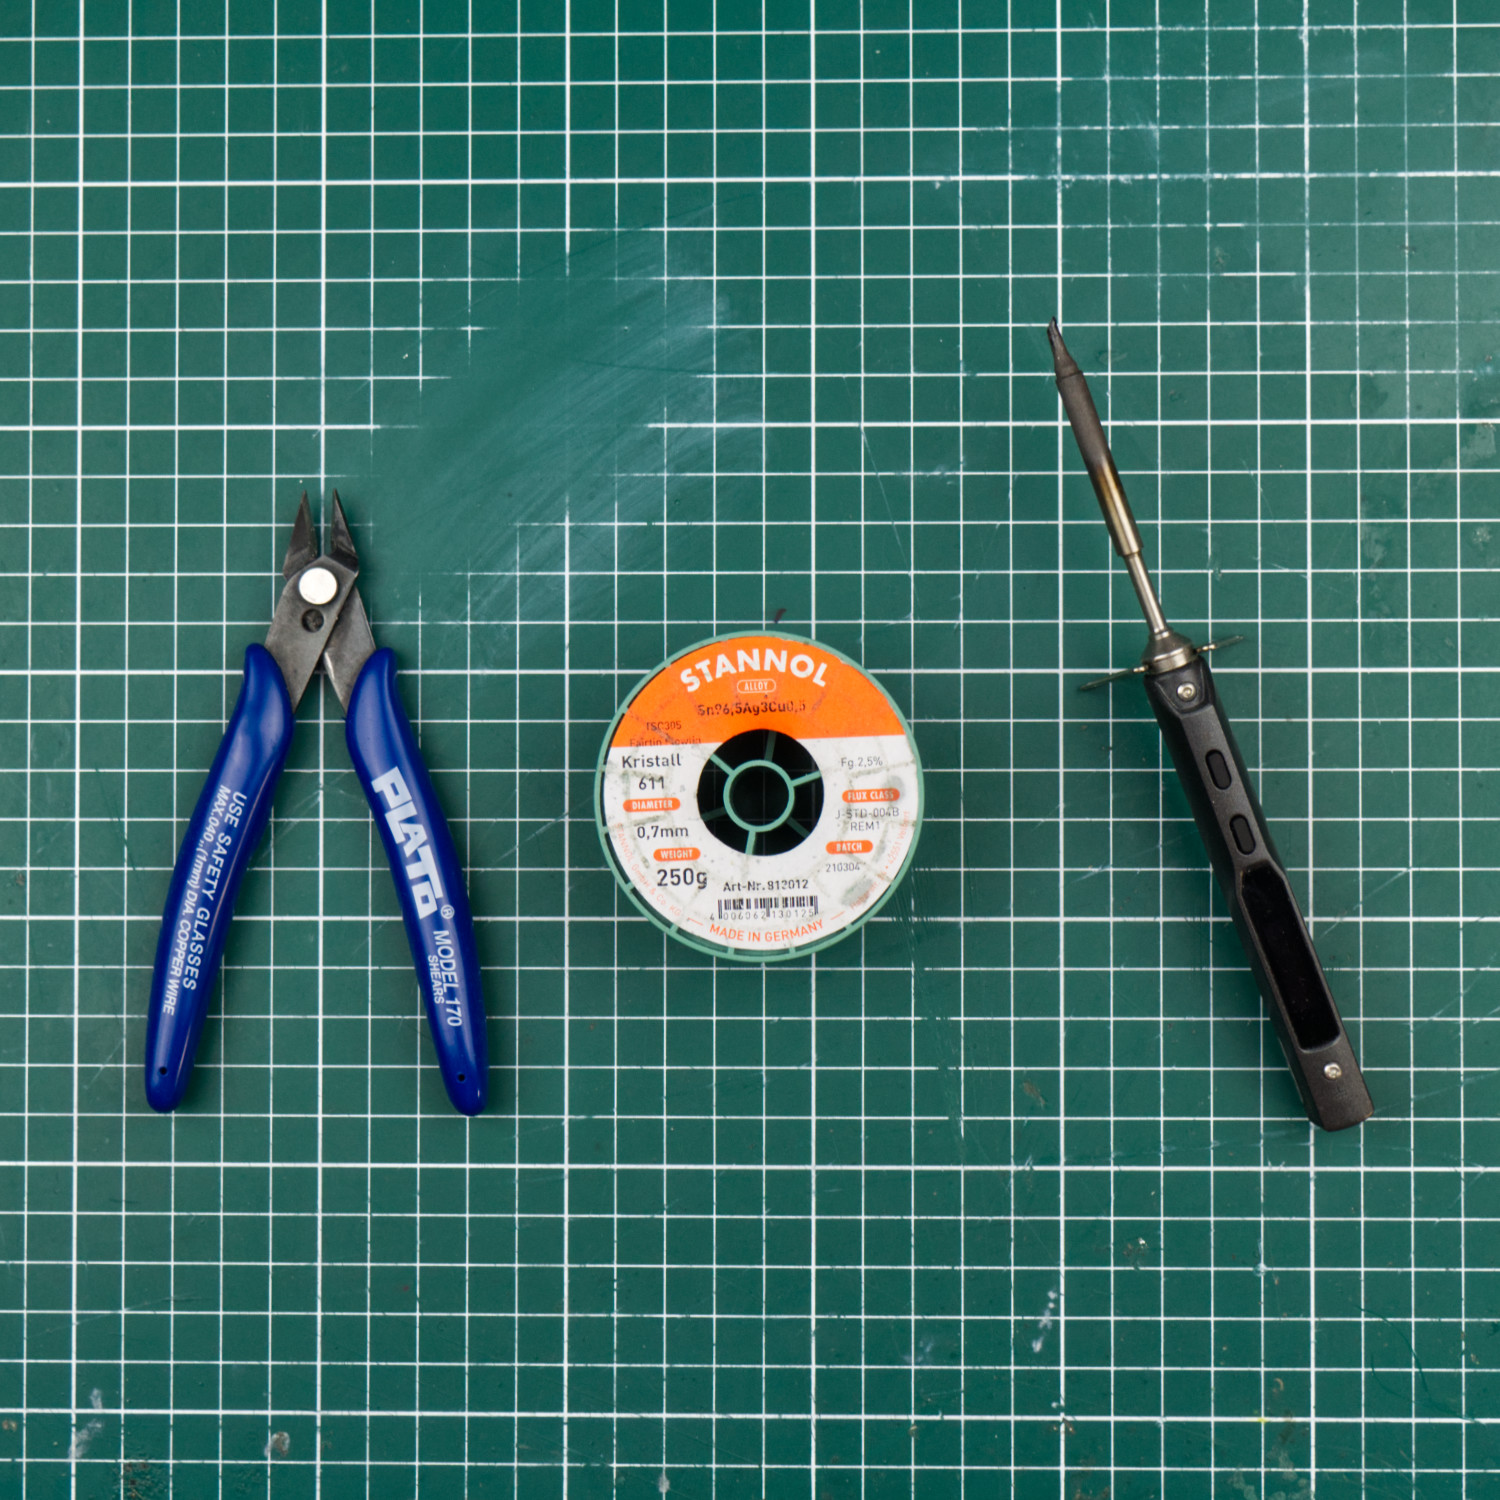
\includegraphics[width=7cm]{images/tools_main.jpg}
    \hspace{2mm}
    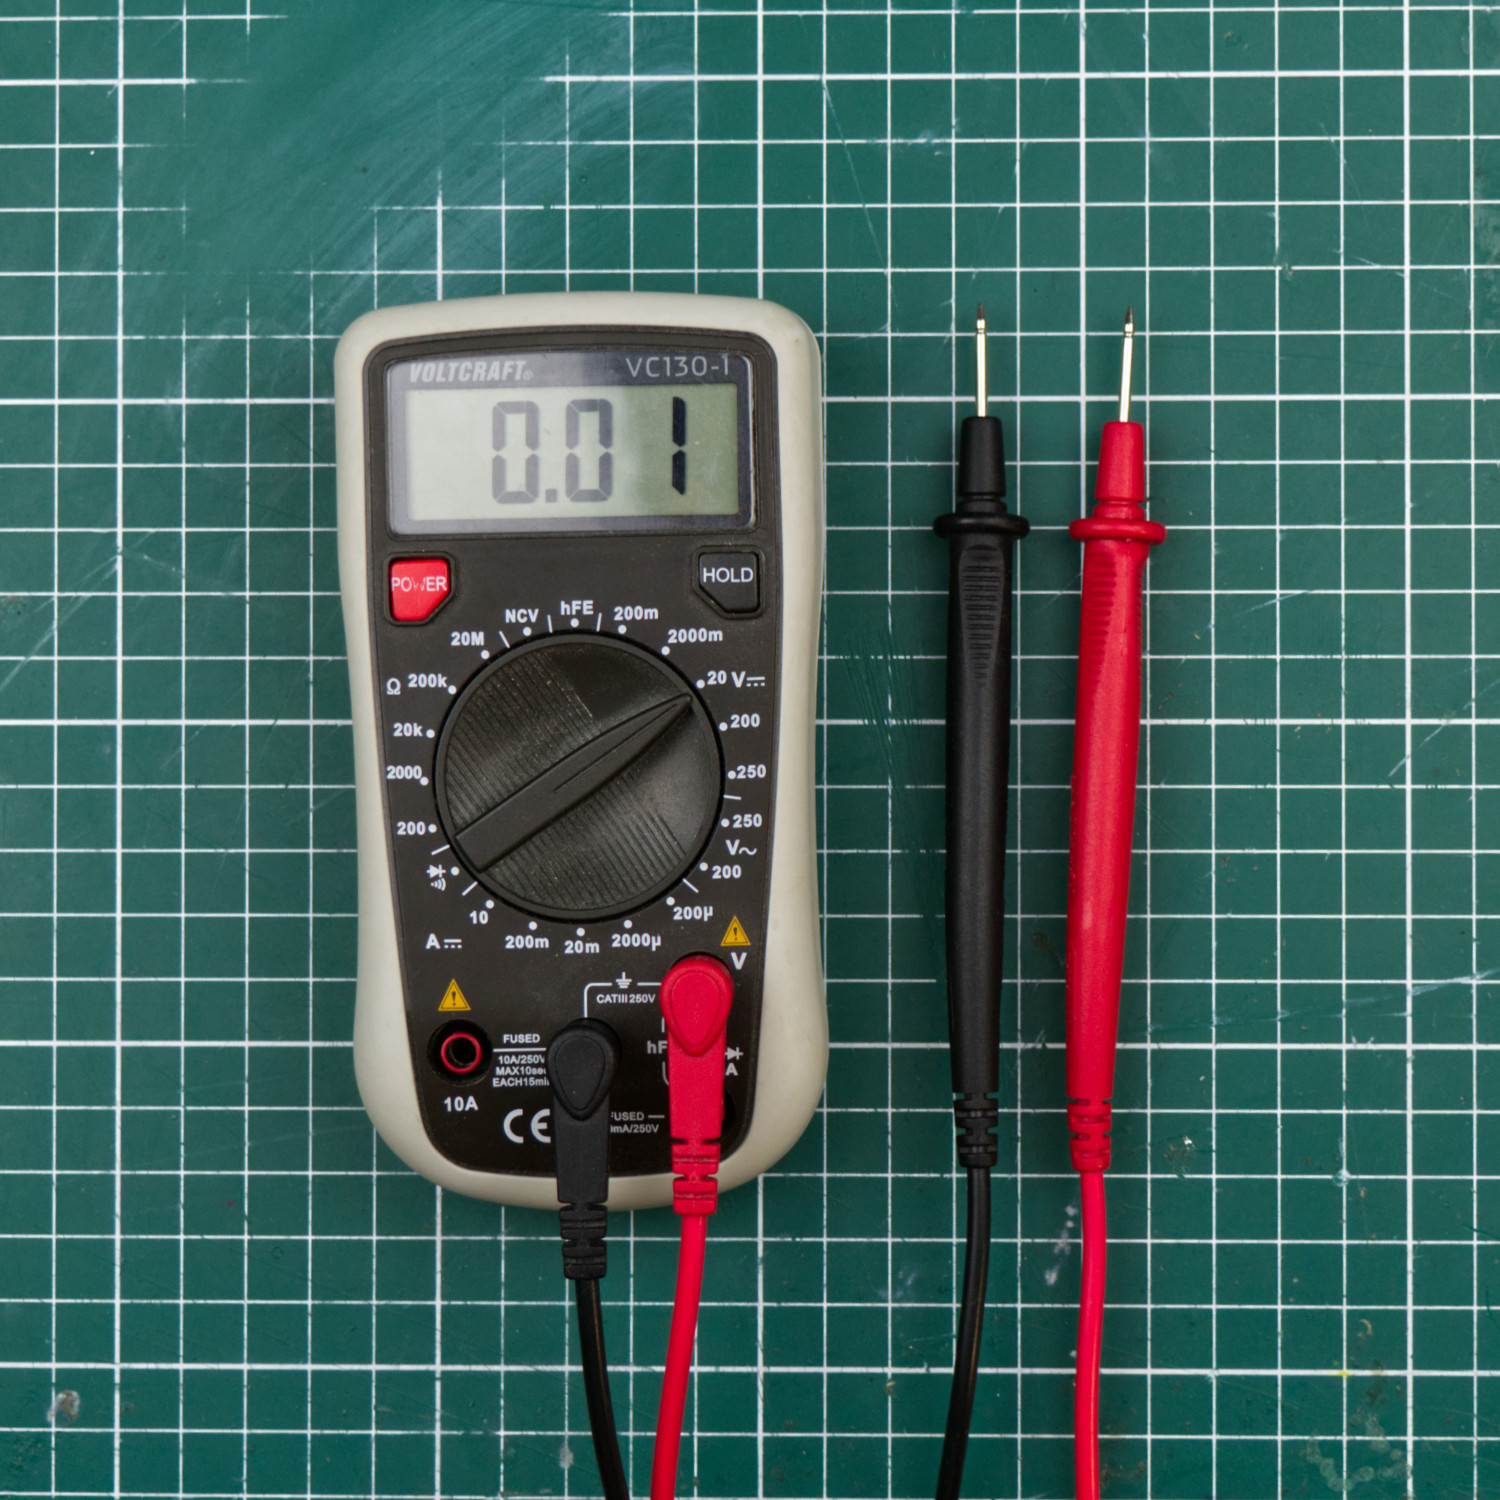
\includegraphics[width=7cm]{images/tools_multimeter.jpg}
\end{figure}

\subsection*{Nice to have}

\begin{itemize}
    \item Solder Wick
    \\ {\small To get rid of superfluous solder.
    Thinner one (\textasciitilde1.0mm \O) tends to work best.}
    \item Magnification
    \\ {\small A simple magnifying glass works nicely to inspect your soldering.}
    \item Ruler/Calipers
    \item Utility Knife
\end{itemize}

\pagebreak
\renewcommand{\contentsname}{Build Steps}
\tableofcontents

\pagebreak
\section{SMD Components}

\begin{figure}[H]
    \centering
    \begin{tikzpicture}
        \node[anchor=south west,inner sep=0] (image) at (0,0) {
            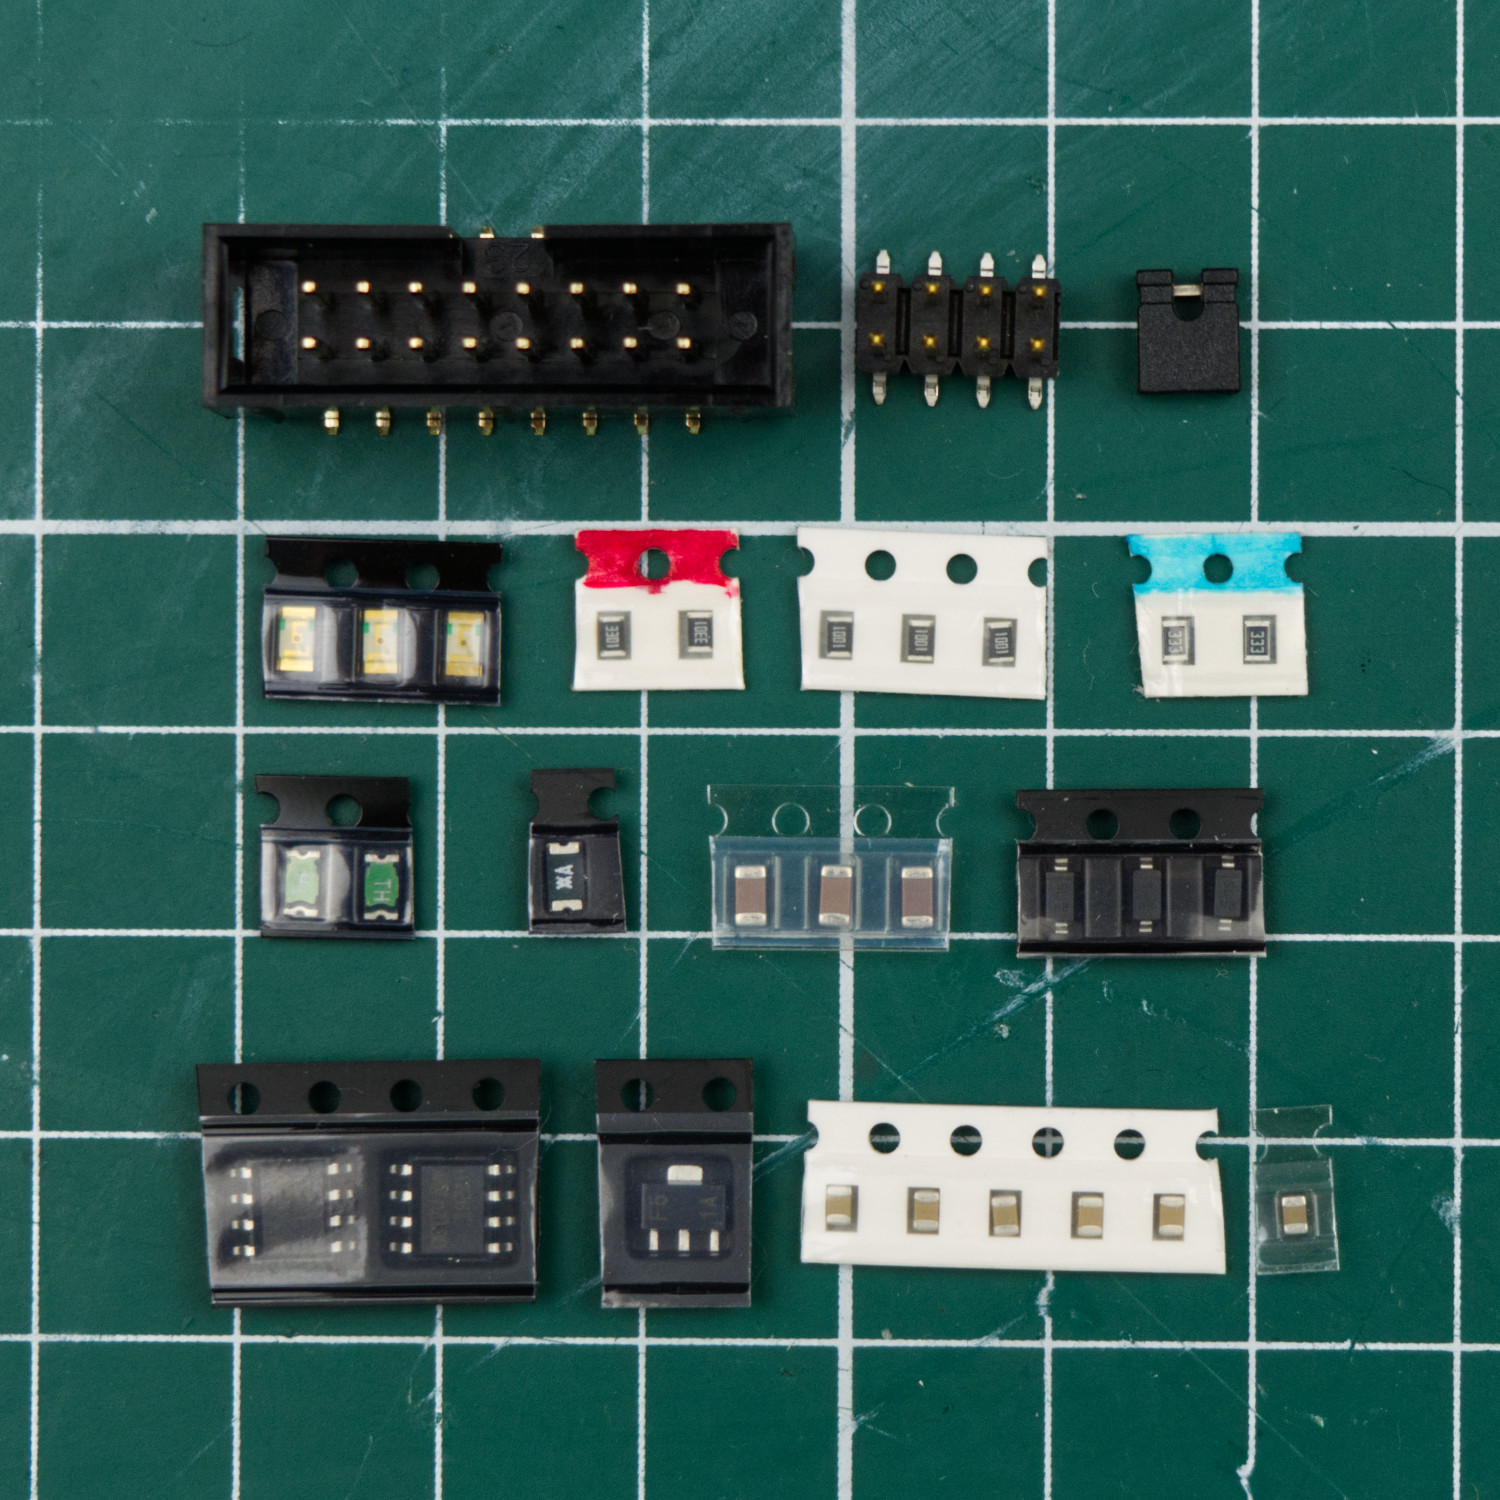
\includegraphics[width=7cm]{images/smt_components_topdown.jpg}
        };
        \begin{scope}[x={(image.south east)},y={(image.north west)}]
            \drawrect{0.13, 0.70}{0.54, 0.86} \drawtext{0.34, 0.82}{1}
            \drawrect{0.56, 0.70}{0.72, 0.86} \drawtext{0.64, 0.82}{2}
            \drawrect{0.74, 0.70}{0.84, 0.86} \drawtext{0.79, 0.82}{3}

            \drawrect{0.15, 0.52}{0.35, 0.66} \drawtext{0.25, 0.62}{4}
            \drawrect{0.37, 0.52}{0.51, 0.66} \drawtext{0.44, 0.62}{5}
            \drawrect{0.52, 0.52}{0.71, 0.66} \drawtext{0.615, 0.62}{6}
            \drawrect{0.74, 0.52}{0.89, 0.66} \drawtext{0.81, 0.62}{7}

            \drawrect{0.15, 0.35}{0.30, 0.49} \drawtext{0.23, 0.45}{8}
            \drawrect{0.33, 0.35}{0.43, 0.49} \drawtext{0.38, 0.45}{9}
            \drawrect{0.46, 0.35}{0.64, 0.49} \drawtext{0.55, 0.45}{10}
            \drawrect{0.66, 0.35}{0.86, 0.49} \drawtext{0.76, 0.45}{11}

            \drawrect{0.12, 0.11}{0.37, 0.31} \drawtext{0.25, 0.26}{12}
            \drawrect{0.39, 0.11}{0.51, 0.31} \drawtext{0.45, 0.26}{13}
            \drawrect{0.53, 0.11}{0.82, 0.31} \drawtext{0.68, 0.26}{14}
            \drawrect{0.83, 0.11}{0.90, 0.31} \drawtext{0.865, 0.26}{15}
        \end{scope}
    \end{tikzpicture}
    \hspace{2mm}
    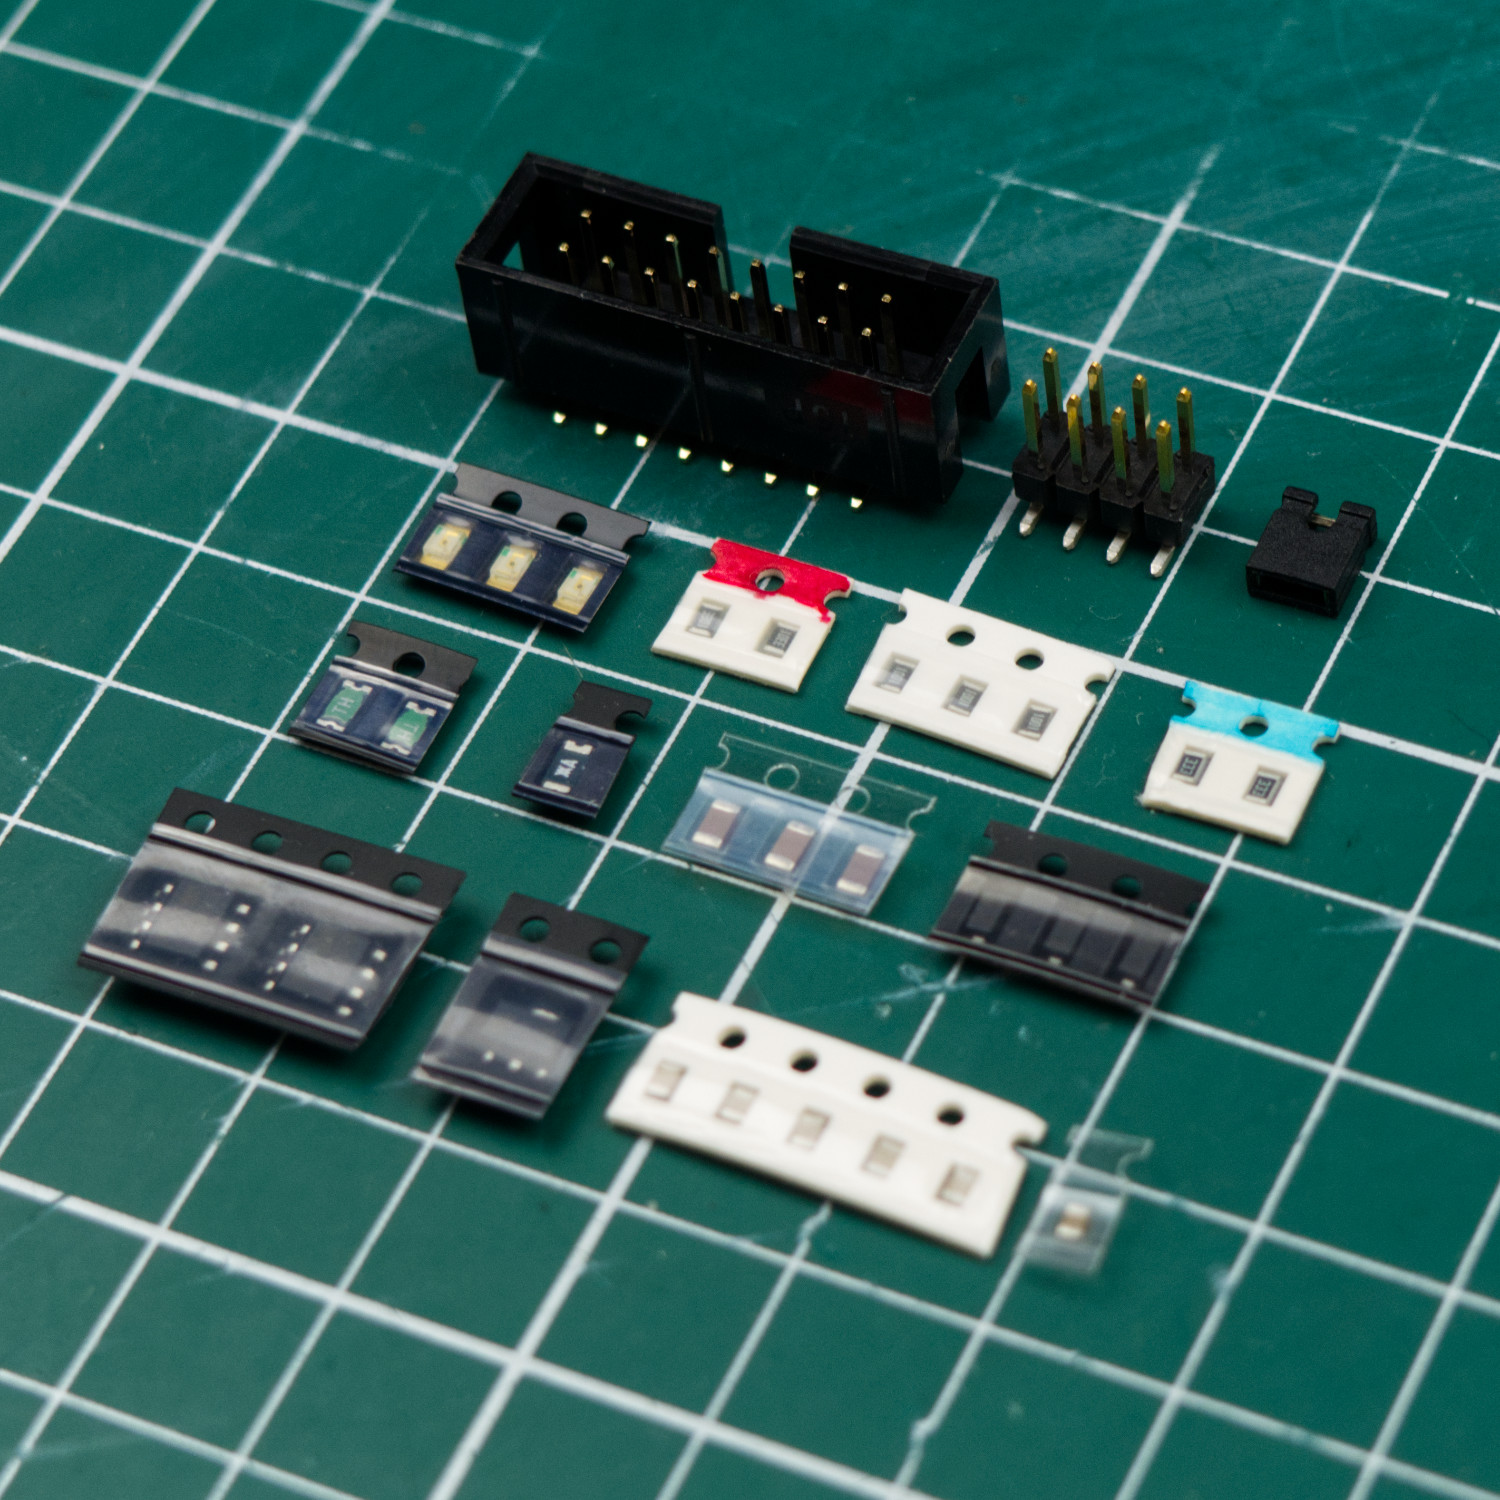
\includegraphics[width=7cm]{images/smt_components_side.jpg}
\end{figure}

\begin{center}
    \small
    \setlength\extrarowheight{4pt}
    \begin{tabularx}{\textwidth}{|c|c|X|l|l|}
        \hline \rowcolor{lightgray} ID & Qty & Description & Code on Part & PCB Identifier / Ref\\
        \hline  1 & 1 & 2×8 IDC Connector & - & J1\\
        \hline  2 & 1 & 2×4 Header & - & J18\\
        \hline  3 & 1 & Jumper & - & -\\
        \hline  4 & 3 & Red LED, 1206 & - & D1, D2, D3\\
        \hline  5 & 3 & \makebox[2em]{\hfill 1k} Resistor, 0805 1\% 1/4W & 1001 & R1, R7, R8\\
        \hline  6 & 2 & \makebox[2em]{\hfill 3.3k} Resistor, 0805 1\%  & 3301 & R2, R3\\
        \hline  7 & 1 & \makebox[2em]{\hfill 10k} Resistor, 0805 1\% & TODO & R9\\
        \hline  8 & 2 & \makebox[2em]{\hfill 33k} Resistor, 0805 0.1\% & 333 & R10, R11\\
        \hline  9 & 1 & \makebox[3.2em]{\hfill 200mA} Resettable Fuse, 1206 & TODO & F1\\
        \hline 10 & 2 & \makebox[3.2em]{\hfill 100mA} Resettable Fuse, 1206 & TODO & F2, F3\\
        \hline 11 & 3 & 10uF Capacitor, 1206 & - & C5, C6, C7\\
        \hline 12 & 3 & 1N5819HW Schottky Diode, SOD-123 & TODO & D4, D5, D6\\
        \hline 13 & 2 & TL072H OpAmp, SOIC8 & TODO & U1, U2\\
        \hline 14 & 1 & L78L05 Voltage Regulator, SOT-89 & TODO & U4\\
        \hline 15 & 1 & LM4040 Voltage Reference, SOT-23 & TODO & U5\\
        \hline 16 & 6 & \makebox[2.8em]{\hfill 100nF} Capacitor, 0805 & - & C1, C2, C3, C4, C10, C11\\
        \hline 17 & 1 & \makebox[2.8em]{\hfill 330nF} Capacitor, 0805 & - & C9\\
        \hline
    \end{tabularx}
\end{center}

\pagebreak

\subsection{Power Protection/Decoupling}

\begin{center}
    \small
    \setlength\extrarowheight{8pt}
    \begin{tabularx}{\textwidth}{|c|c|c|X|l|l|}
        \hline\rowcolor{lightgray} & ID & Qty & Description & Code on Part & PCB Identifier\\
        \hline\checkbox{aa} & 12 & 3 & 1N5819HW Schottky Diode, SOD-123 & TODO & D4, D5, D6\\
        \hline\checkbox{ab} & 11 & 3 & 10uF Capacitor, 1206 & - & C5, C6, C7\\
        \hline\checkbox{ac} & 10 & 2 & \makebox[3.2em]{\hfill 100mA} Resettable Fuse, 1206 & TODO & F2, F3\\
        \hline\checkbox{ad} &  9 & 1 & \makebox[3.2em]{\hfill 200mA} Resettable Fuse, 1206 & TODO & F1\\
        \hline
    \end{tabularx}
\end{center}

Start by soldering the 1N5819HW Schottky diodes and 10uF decoupling capacitors for each of the
three power rails. \textbf{Mind the polarity of the diodes!}

Then, do the same for the resettable PTC fuses. The two green ones are for the +12V and -12V
power rails and can hold a maximum current of 100mA indefinitely and will trip at
\textasciitilde 250mA. The black one is for the +5V rail and has a hold current of 200mA and
will trip at \textasciitilde 400mA. (This should be enough for most circuits, even ones
including power-hungry digital microcontrollers.)

\begin{figure}[H]
    \centering
    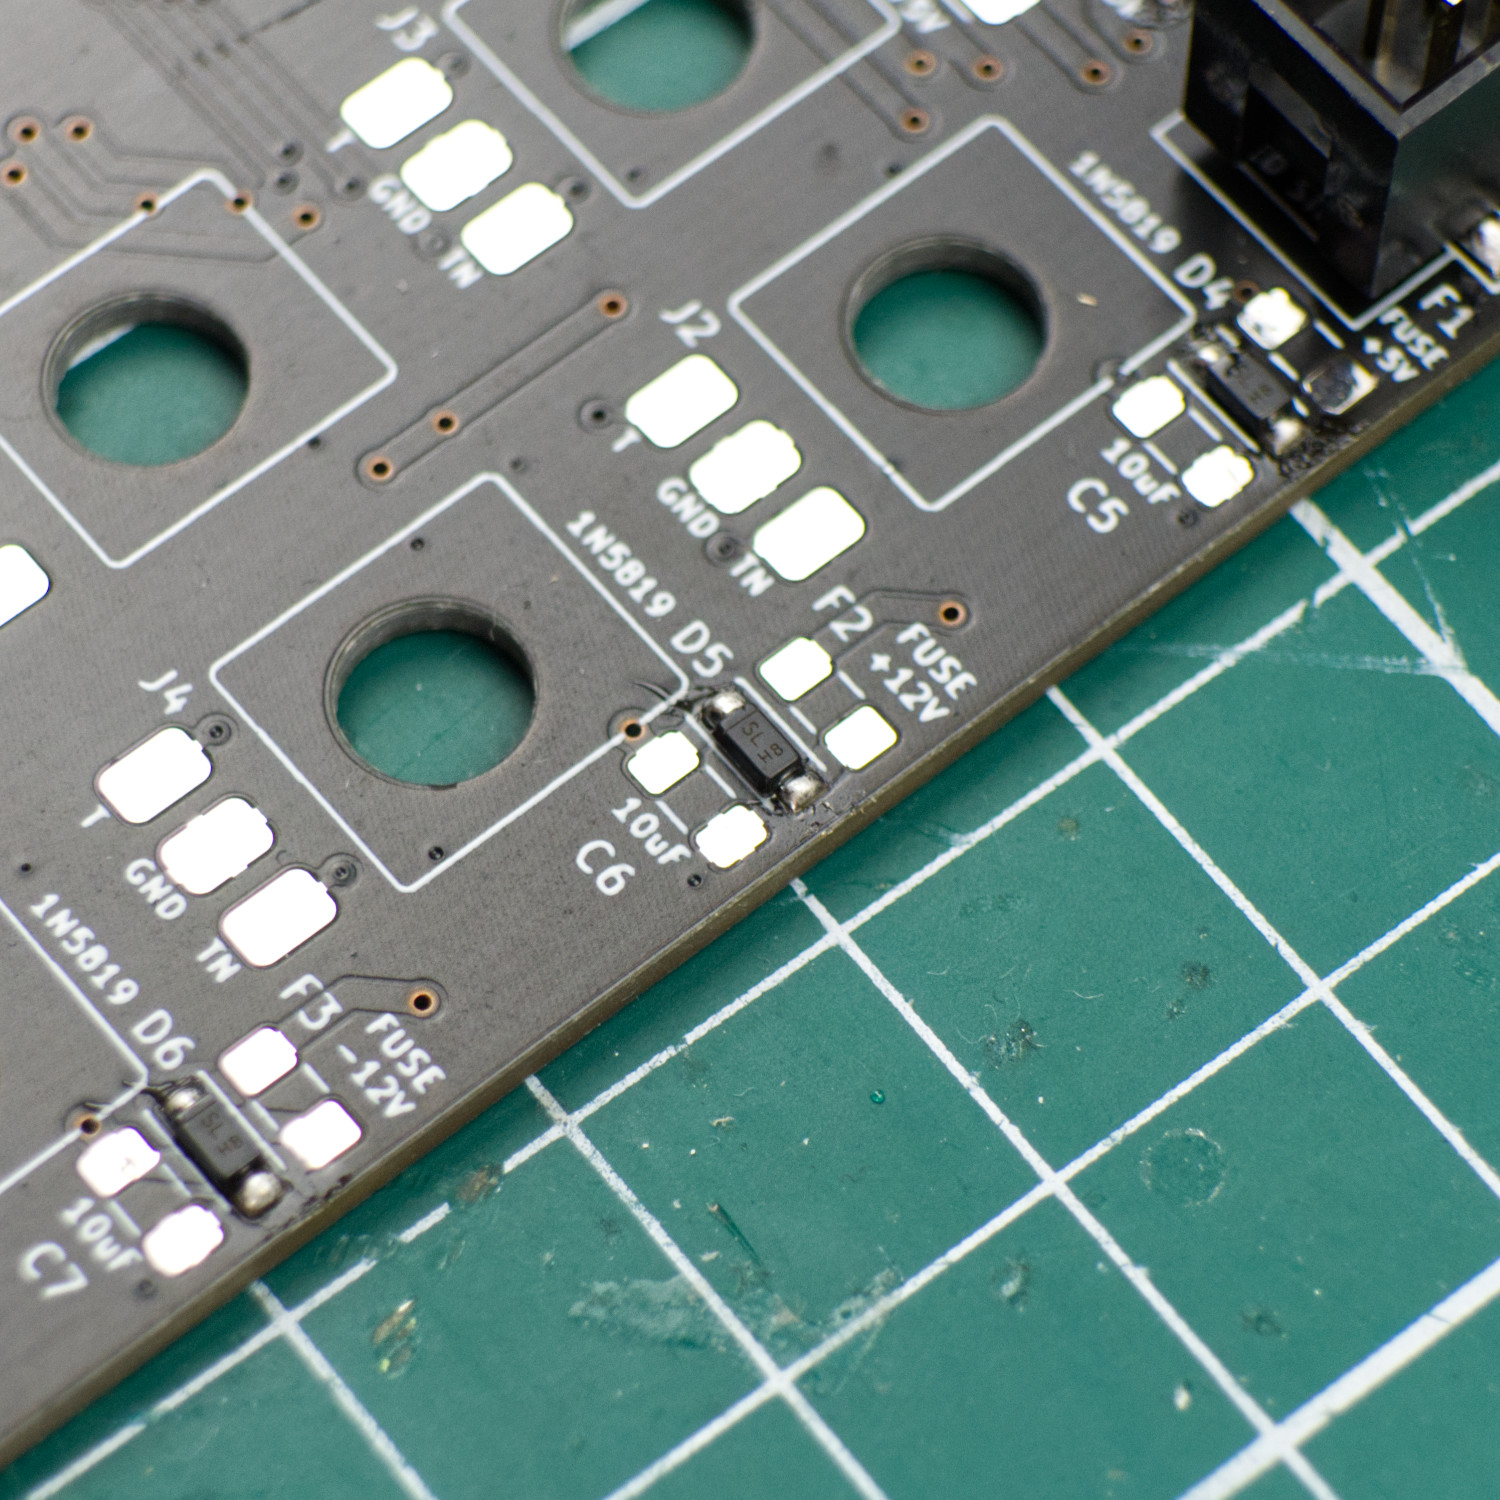
\includegraphics[width=46mm]{images/section_1-1_diodes.jpg}
    \hspace{2mm}
    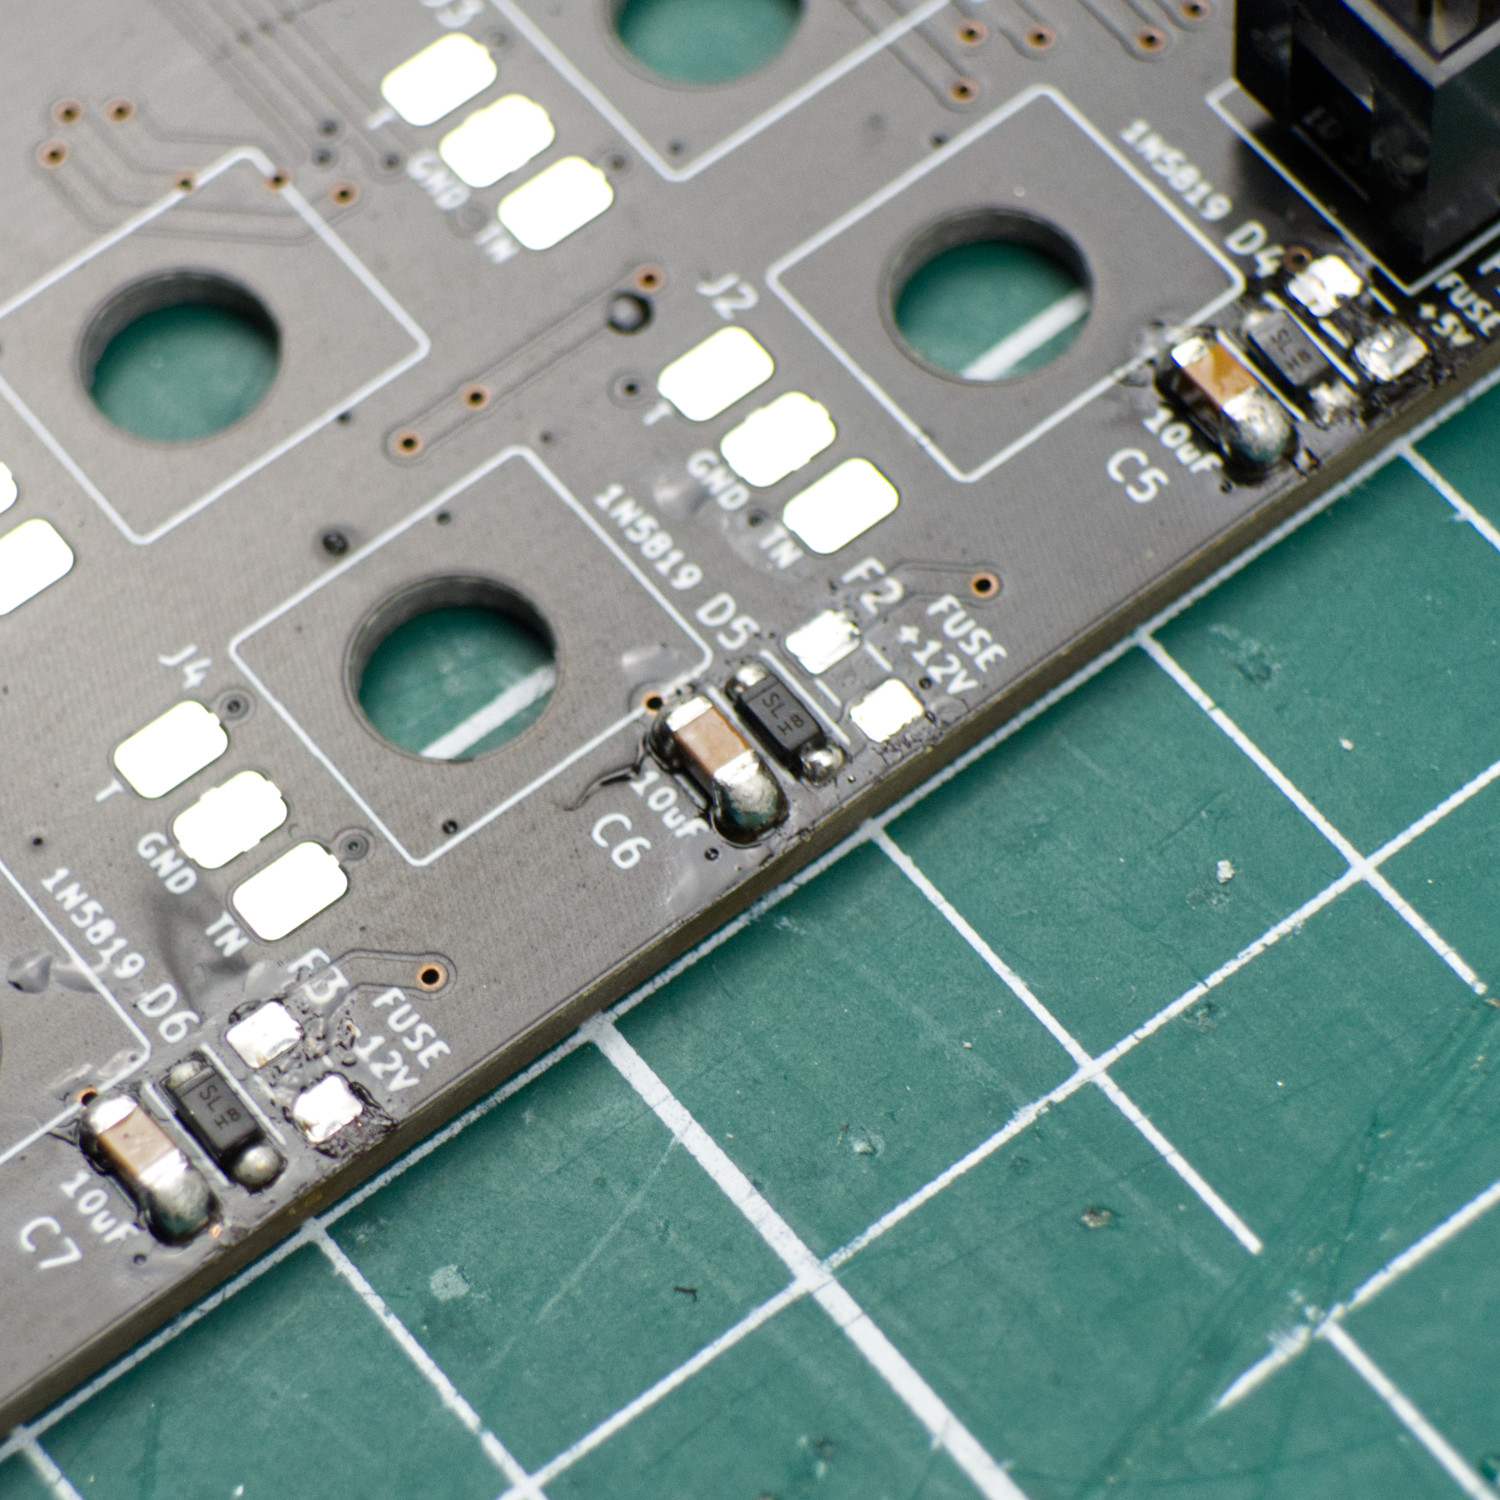
\includegraphics[width=46mm]{images/section_1-1_capacitors.jpg}
    \hspace{2mm}
    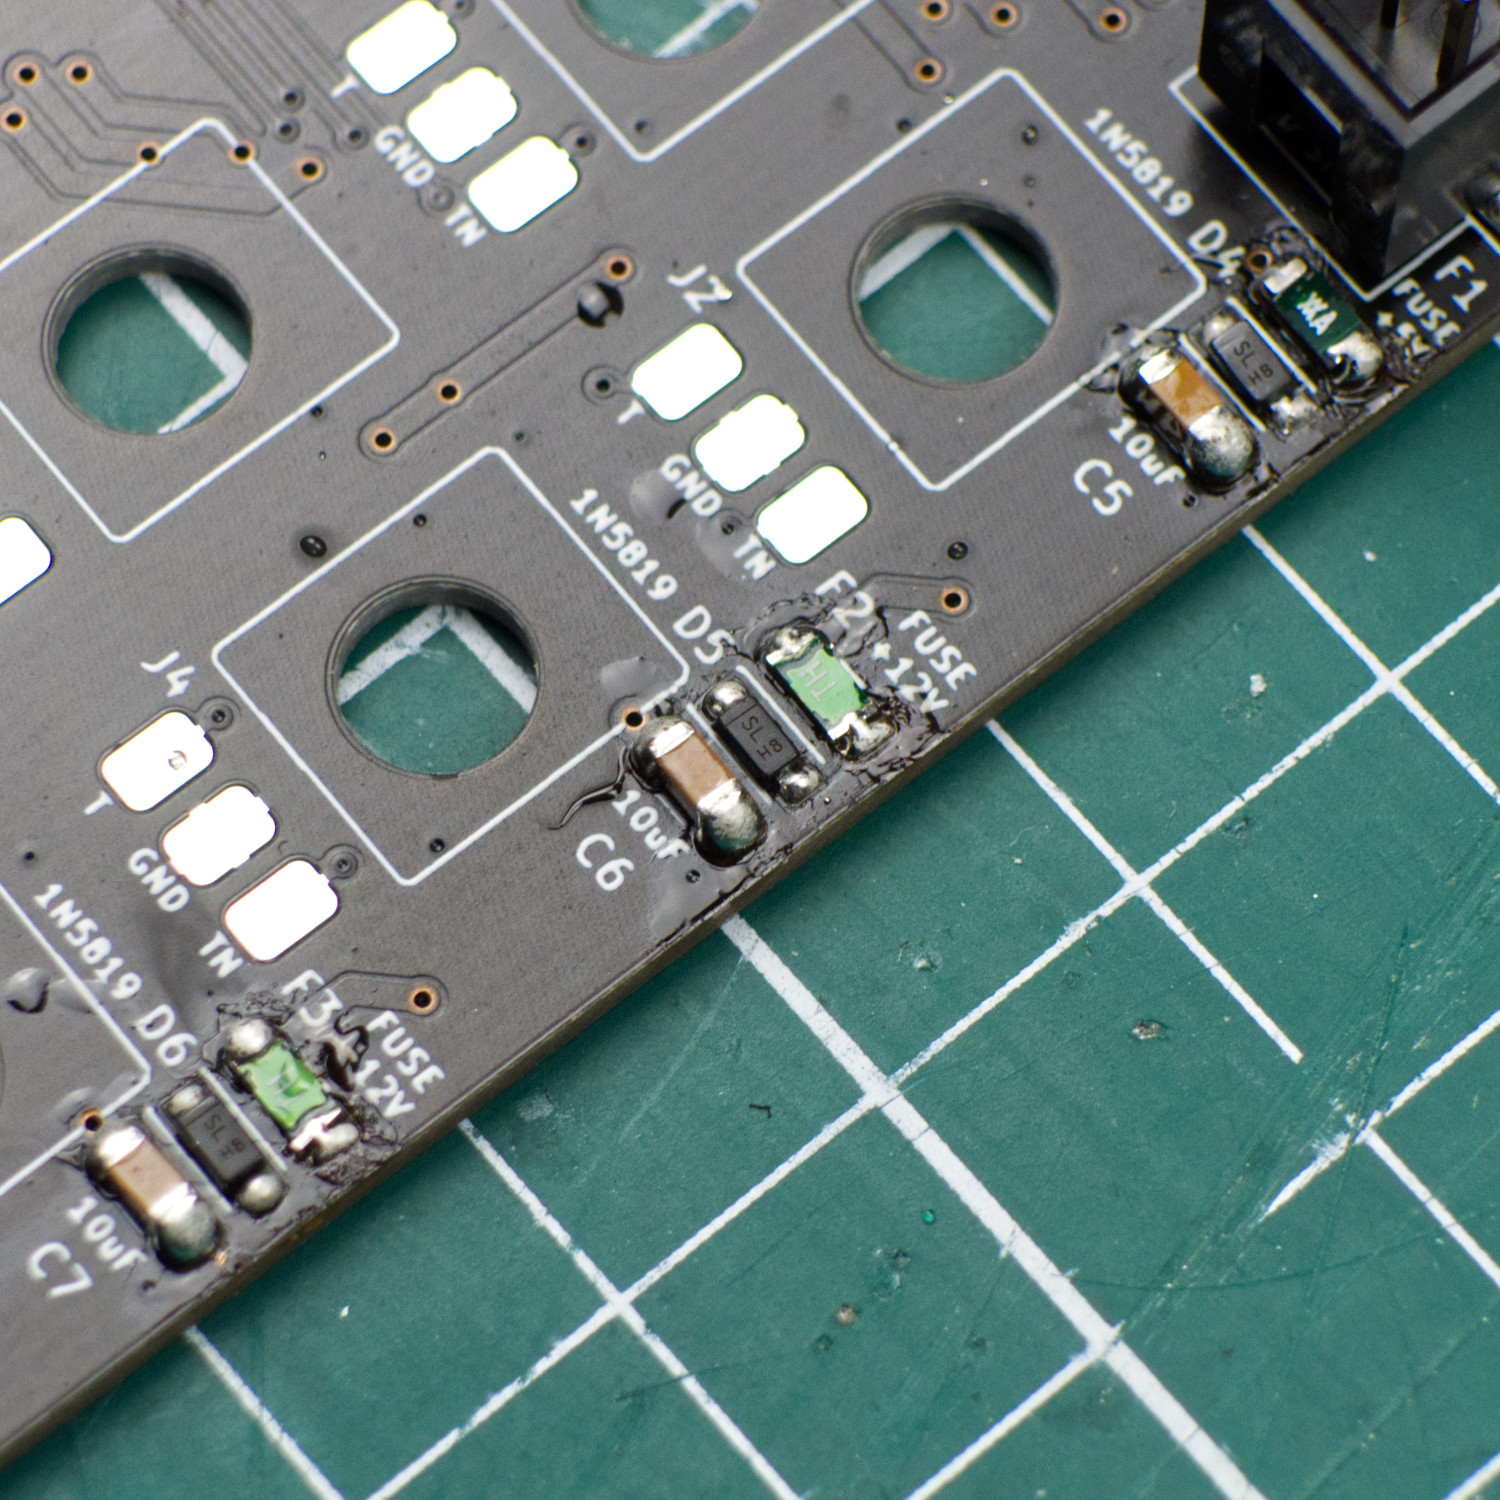
\includegraphics[width=46mm]{images/section_1-1_fuses.jpg}
\end{figure}

\begin{quoting}
    \small
    (If you plan on building circuits that require more current, you can replace the fuses with
    ones that support a higher hold current, \textbf{making sure your power supply can still
    supply their rated trip current!})
\end{quoting}

\subsection{Power Connector, LEDs}

\begin{center}
    \small
    \setlength\extrarowheight{8pt}
    \begin{tabularx}{\textwidth}{|c|c|c|X|l|l|}
        \hline\rowcolor{lightgray} & ID & Qty & Description & Code on Part & PCB Identifier\\
        \hline\checkbox{ba} & 6 & 2 & \makebox[2em]{\hfill 3.3k} Resistor, 0805 1\%  & 3301 & R2, R3\\
        \hline\checkbox{bb} & 5 & 1 & \makebox[2em]{\hfill 1k} Resistor, 0805 1\% & 1001 & R1\\
        \hline\checkbox{bc} & 1 & 1 & 2×8 IDC Connector & - & J1\\
        \hline\checkbox{bd} & 4 & 3 & Red LED, 1206 & - & D1, D2, D3\\
        \hline
    \end{tabularx}
\end{center}

Start by soldering the two 3.3k resistors and the 1k resistor.

Next is the power connector. Align it carefully,
\textbf{minding its orientation (there is an arrow on one side, which has to
align with the white stripe on the PCB)} and solder it in place. Closely inspect your soldering
and ensure you do not have any shorts, as this area will be hard to access later on.

Finally, solder the LEDs. These have to be soldered upside-down so that they can shine through
the board. There is a T-shaped marking on their back that has to be aligned with the matching
symbol on the PCB. \textbf{{Be careful not to overheat the LEDs! The plastic
lenses can be damaged quite easily!}}

\begin{figure}[H]
    \centering
    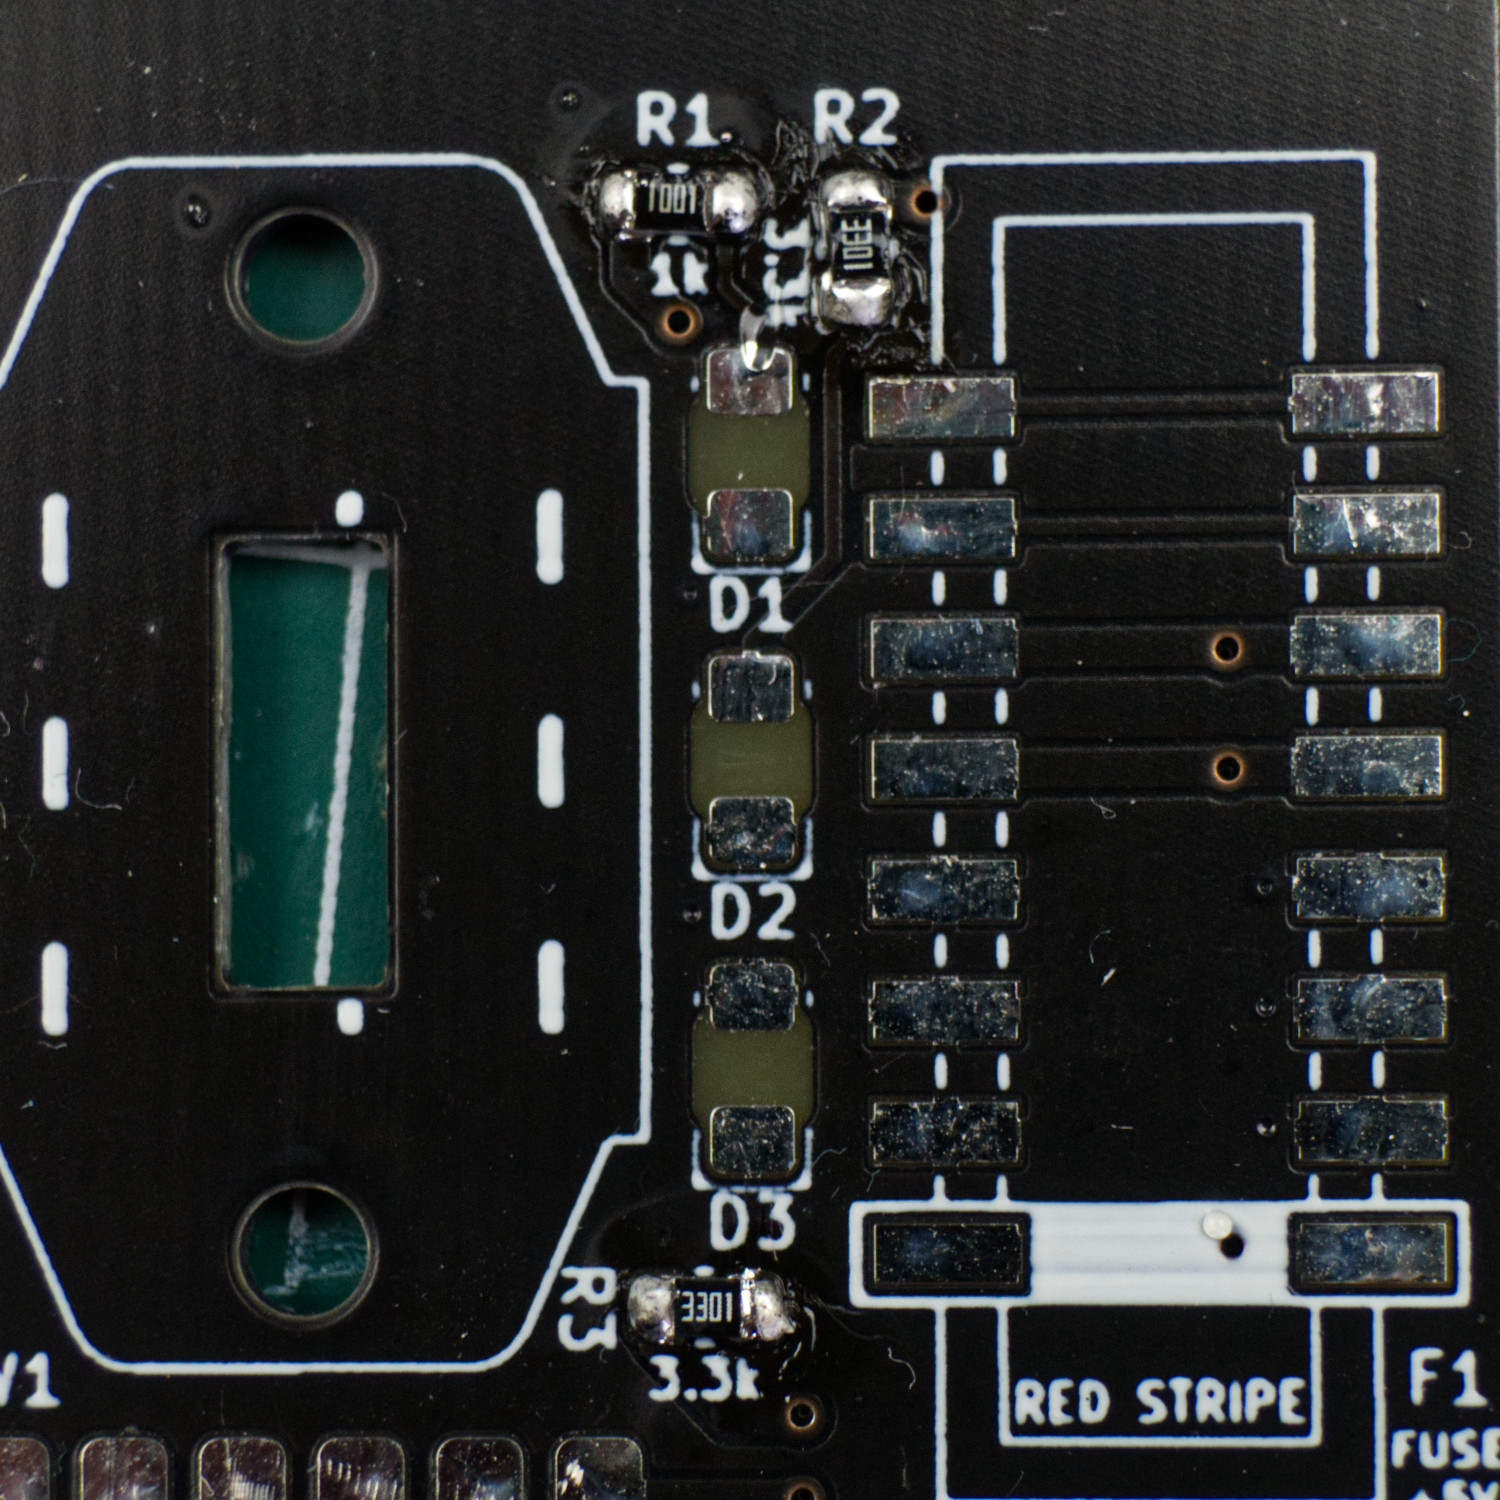
\includegraphics[width=46mm]{images/section_1-2_resistors.jpg}
    \hspace{2mm}
    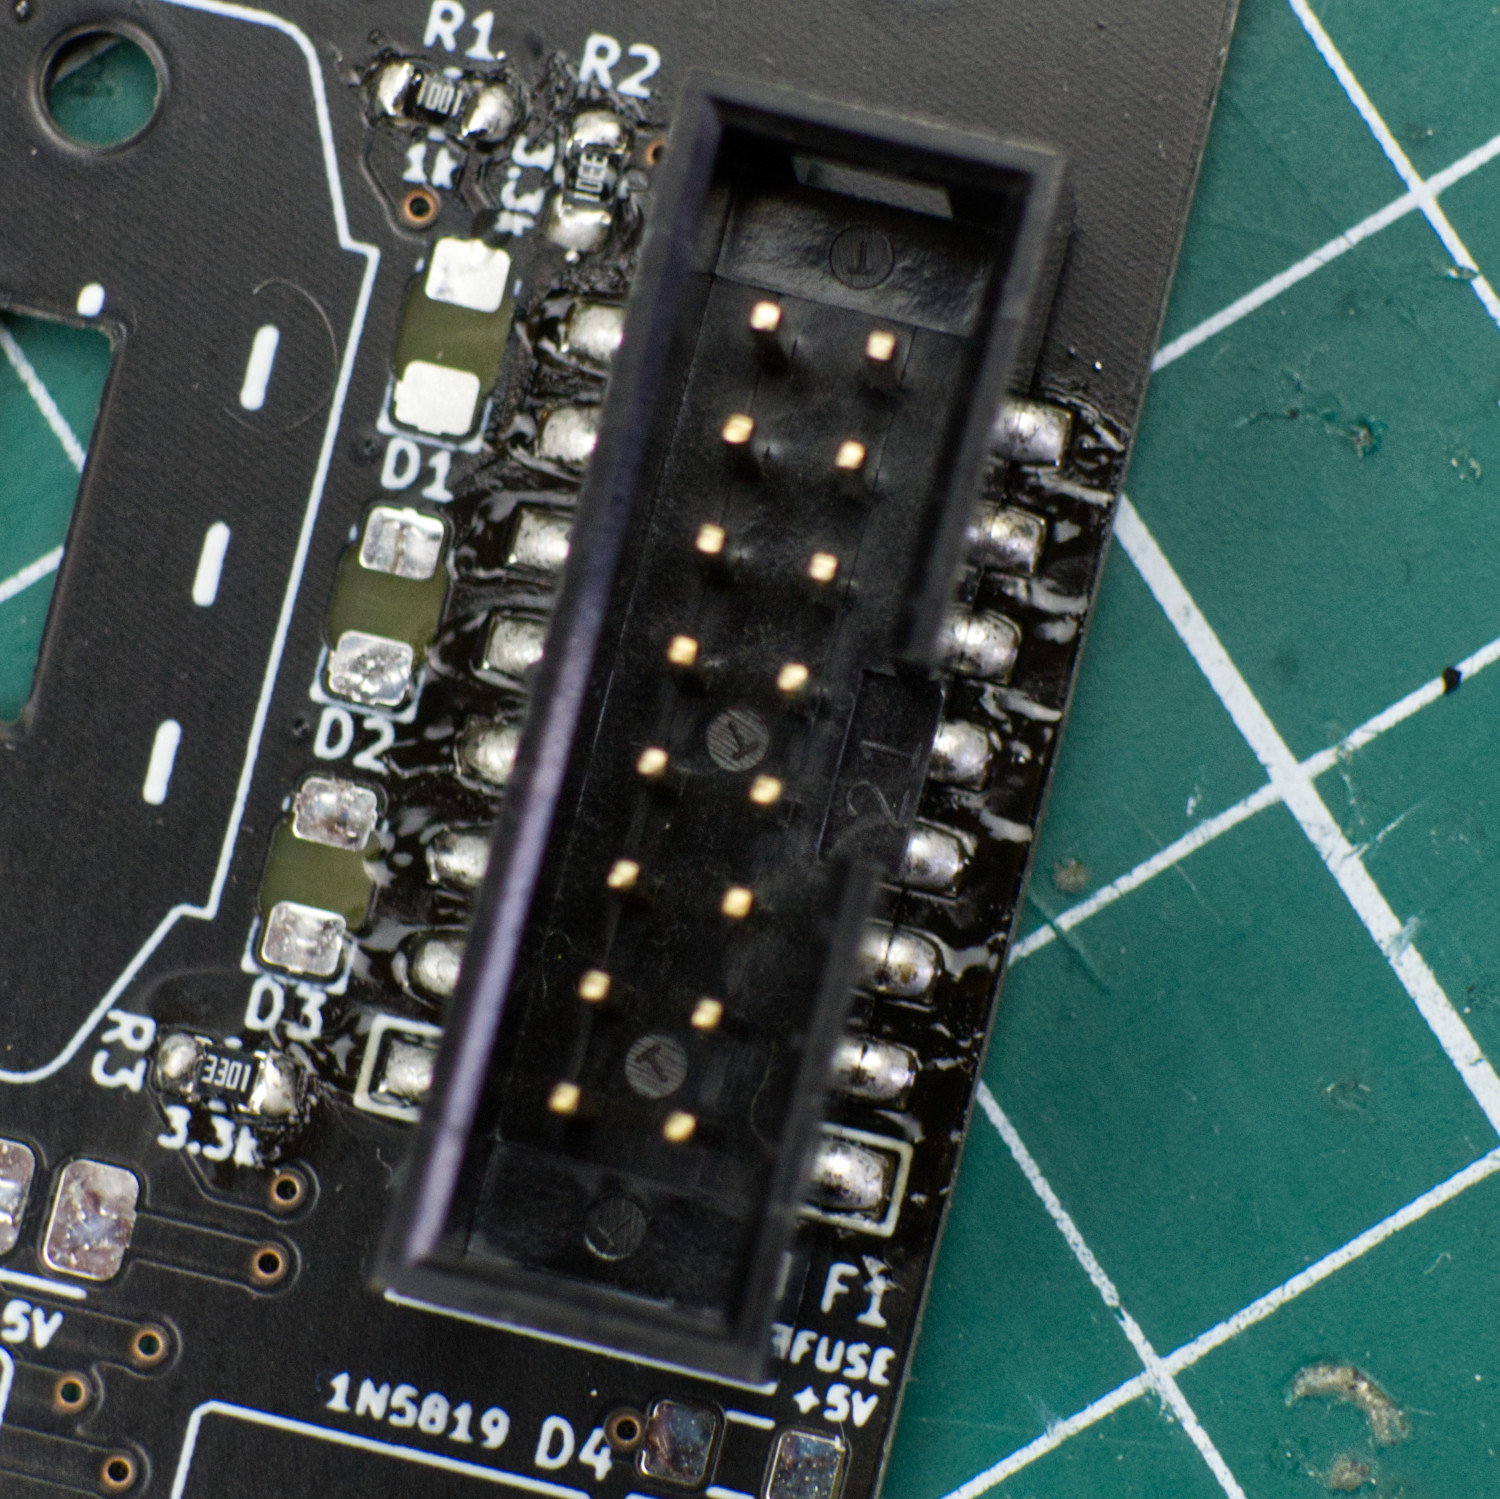
\includegraphics[width=46mm]{images/section_1-2_powerconnector.jpg}
    \hspace{2mm}
    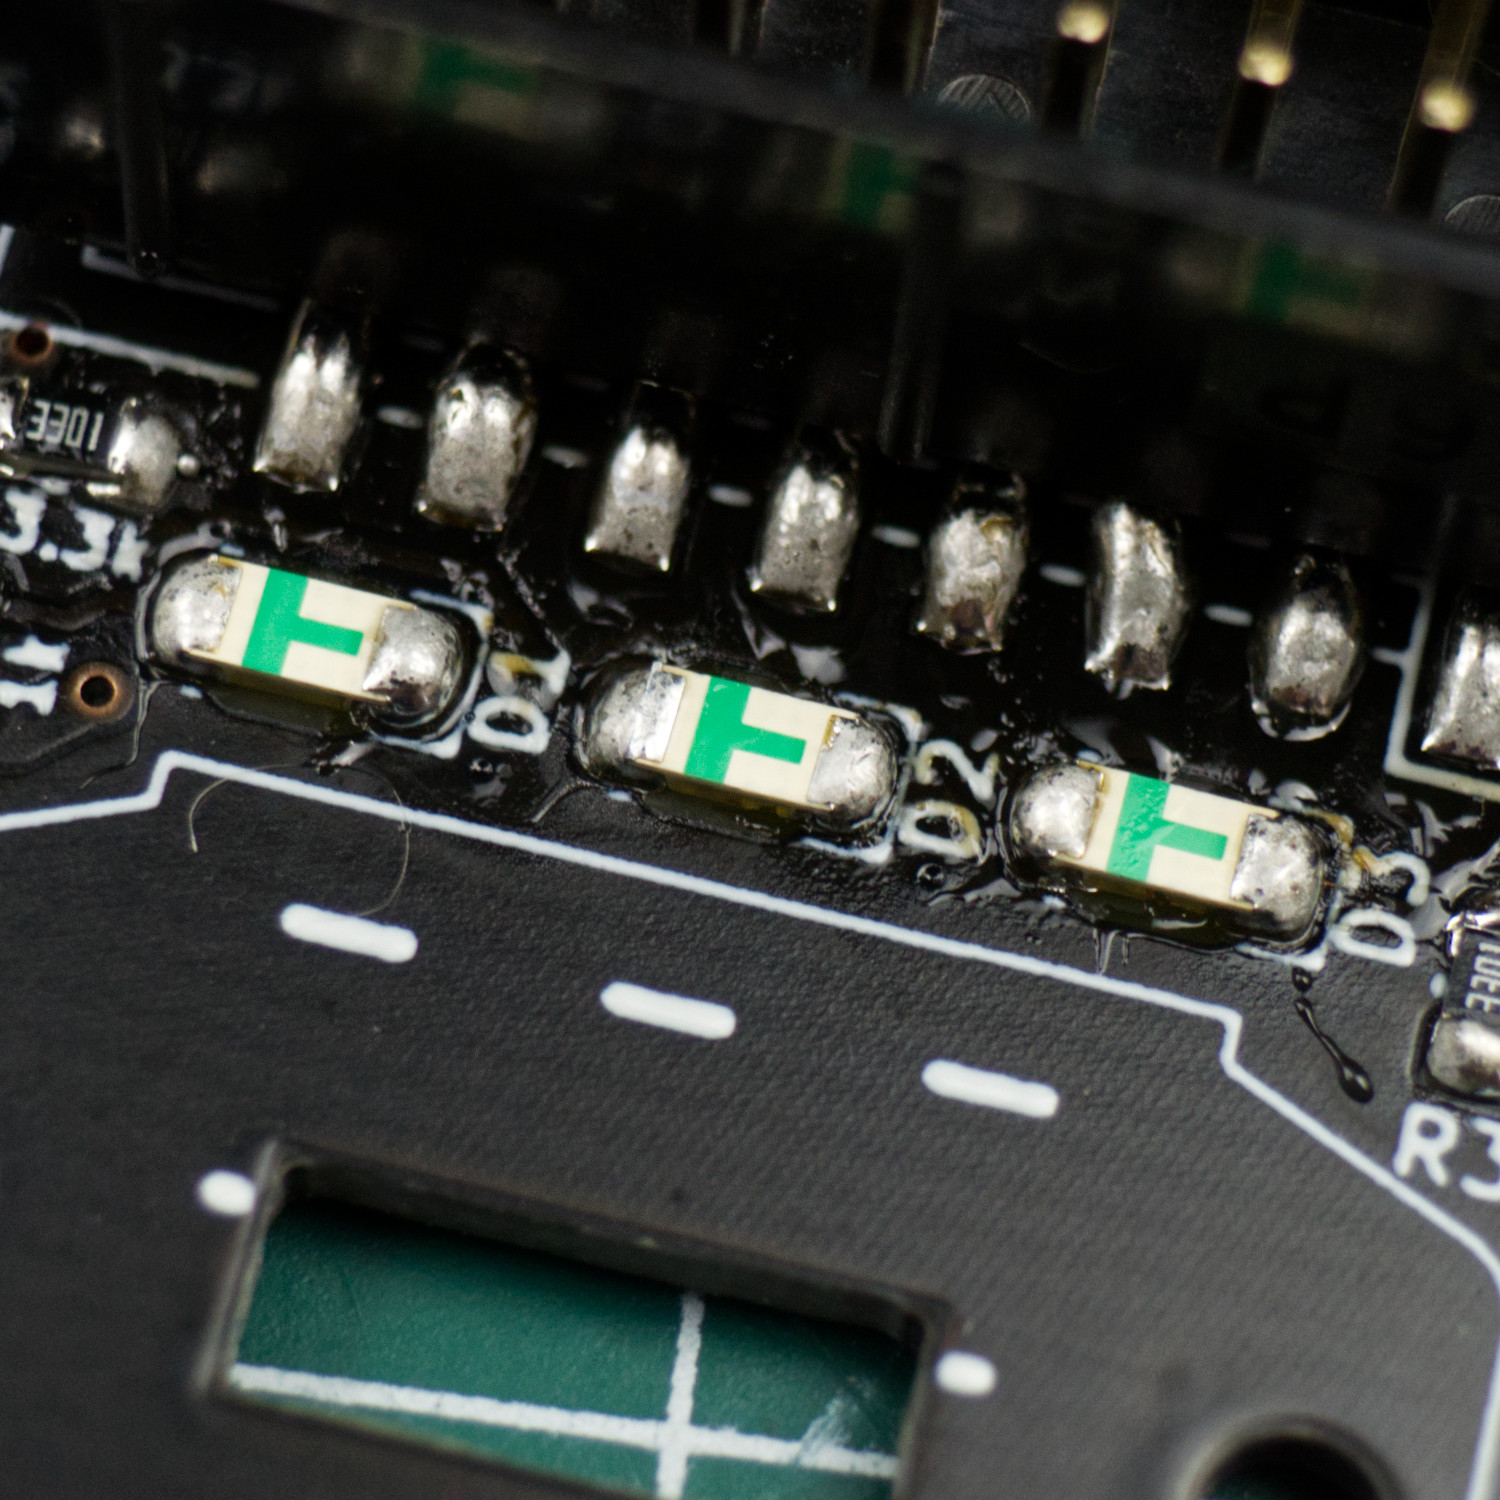
\includegraphics[width=46mm]{images/section_1-2_leds.jpg}
\end{figure}

\subsection{Buffered Outputs}

\begin{center}
    \small
    \setlength\extrarowheight{8pt}
    \begin{tabularx}{\textwidth}{|c|c|c|X|l|l|}
        \hline\rowcolor{lightgray} & ID & Qty & Description & Code on Part & PCB Identifier\\
        \hline\checkbox{ca} & 13 & 1 & TL072H OpAmp, SOIC8 & TODO & U1\\
        \hline\checkbox{cb} & 16 & 2 & 100nF Capacitor, 0805 & - & C1, C2\\
        \hline\checkbox{cc} &  5 & 2 & 1k Resistor, 0805 1\% 1/4W & 1001 & R7, R8\\
        \hline
    \end{tabularx}
\end{center}

First, solder the TL072B. Make sure to line up the little dot that marks Pin 1 with the marker
on the PCB.

Then, solder the 100nF decoupling capacitors and the 1k outputs resistors.

\begin{figure}[H]
    \centering
    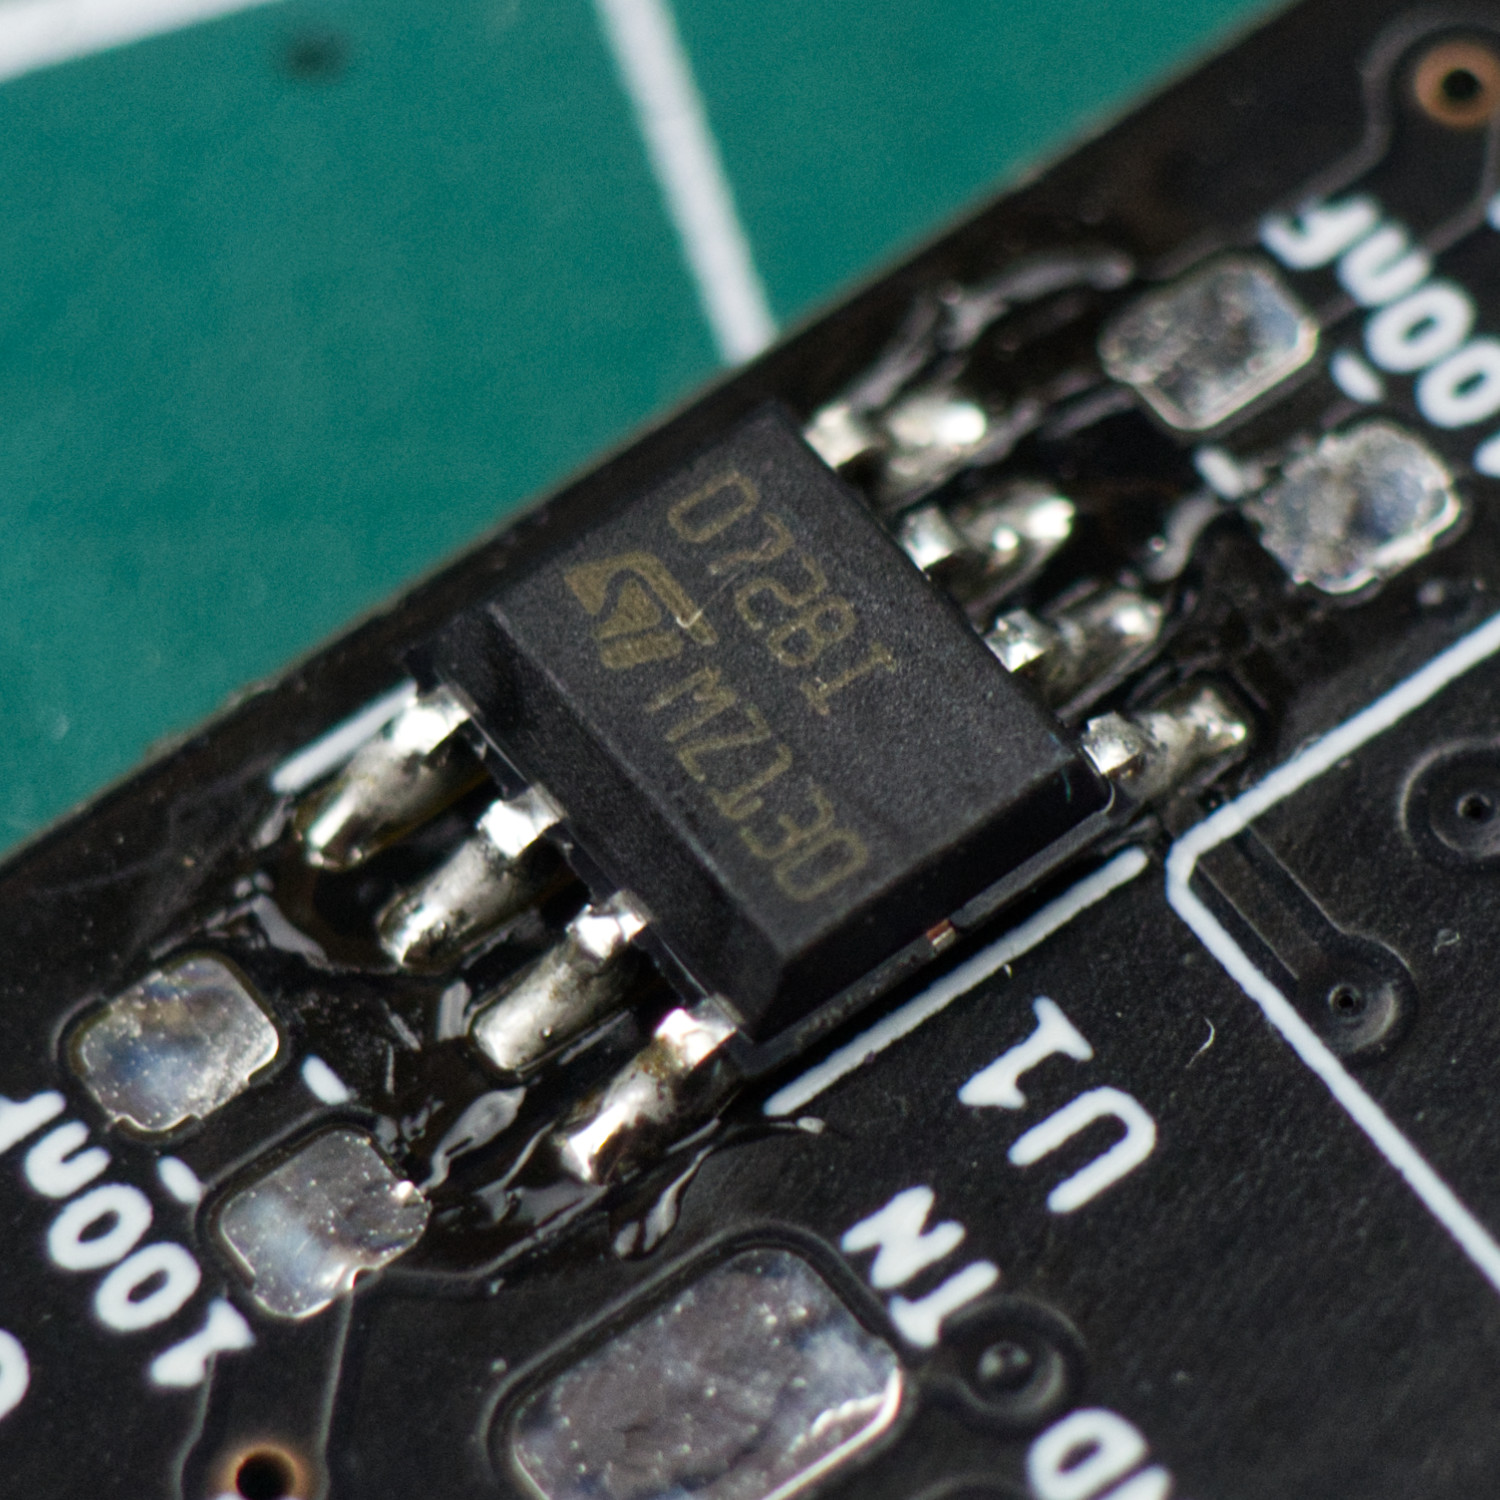
\includegraphics[width=46mm]{images/section_1-3_opamp.jpg}
    \hspace{2mm}
    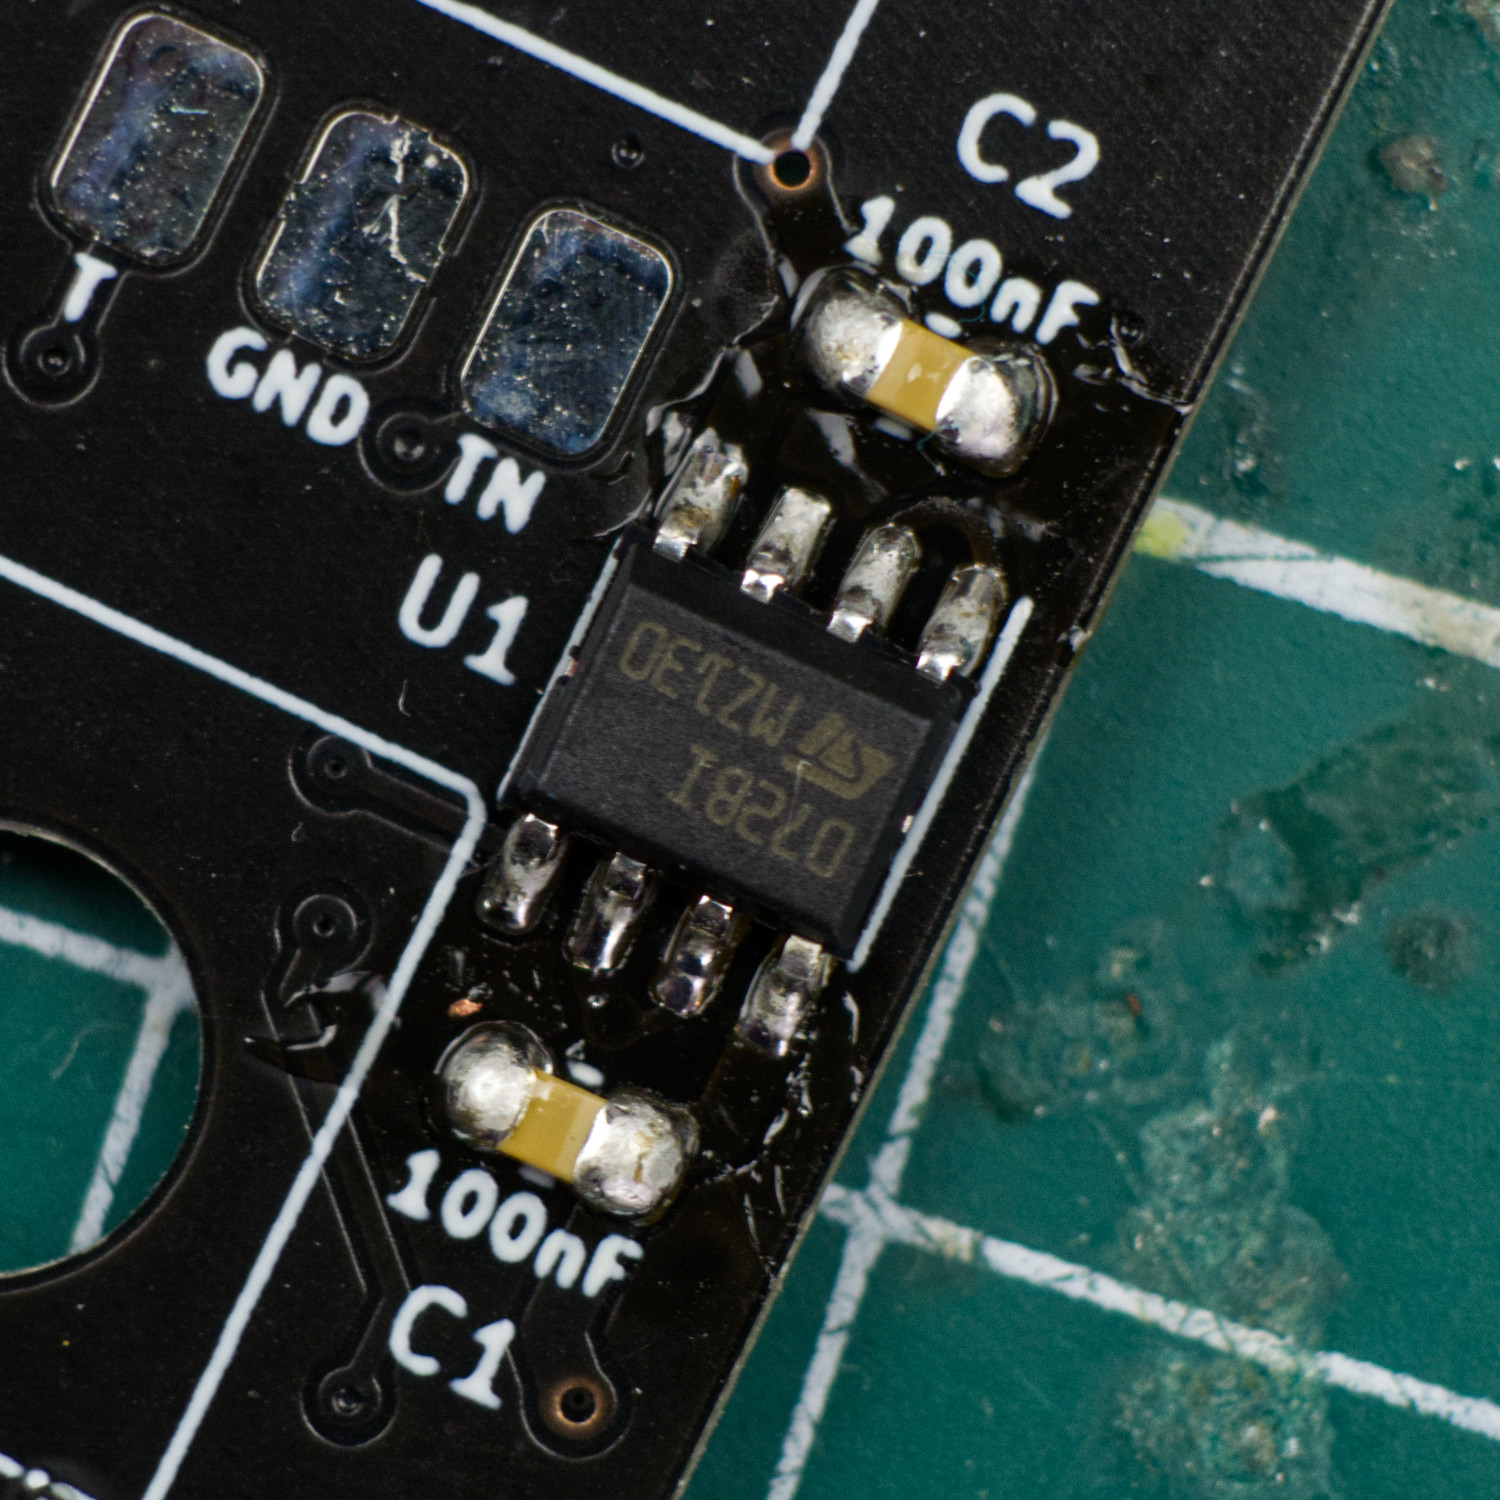
\includegraphics[width=46mm]{images/section_1-3_capacitors.jpg}
    \hspace{2mm}
    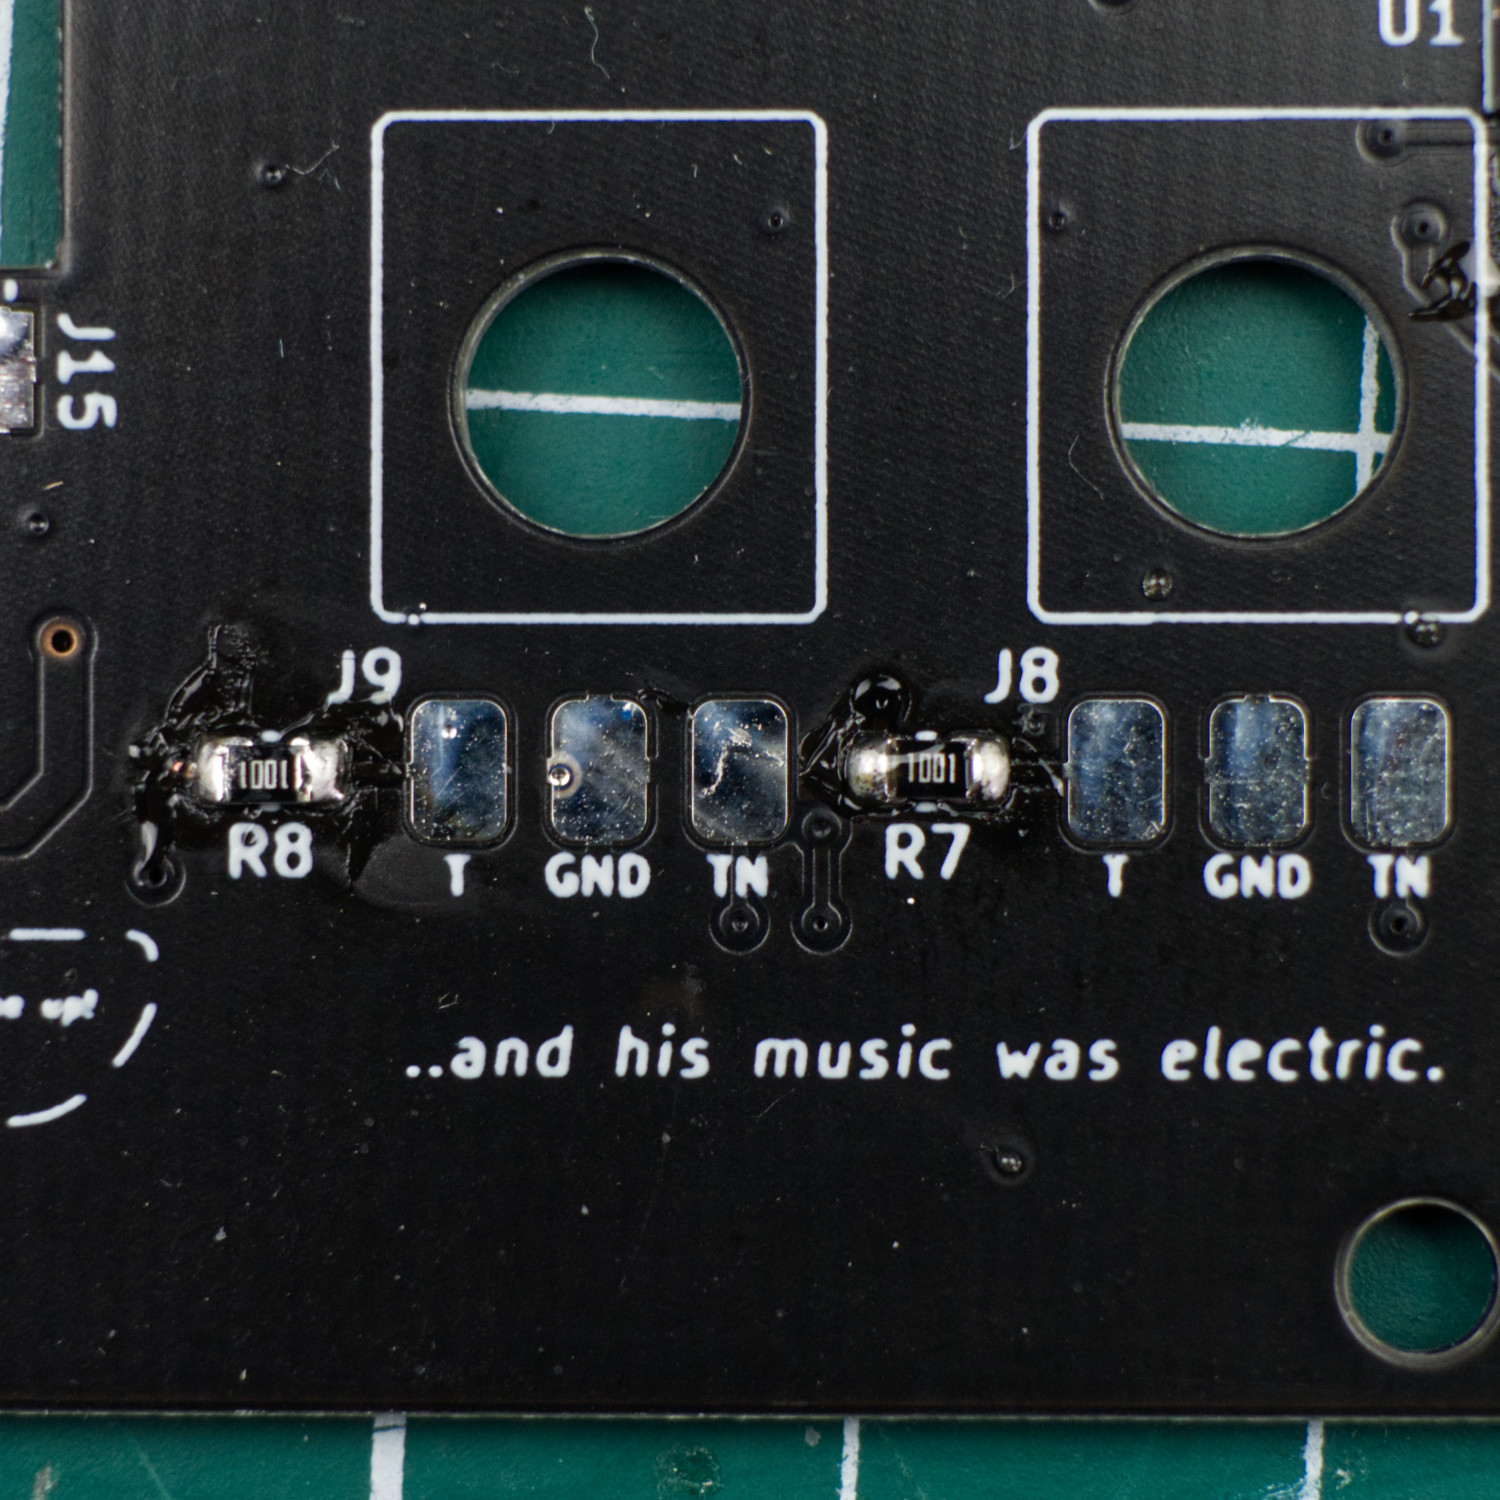
\includegraphics[width=46mm]{images/section_1-3_resistors.jpg}
\end{figure}

\subsection{Reference Voltage Buffer}
\label{sec:reference_voltage_buffer}

\begin{center}
    \small
    \setlength\extrarowheight{8pt}
    \begin{tabularx}{\textwidth}{|c|c|c|X|l|l|}
        \hline\rowcolor{lightgray} & ID & Qty & Description & Code on Part & PCB Identifier\\
        \hline\checkbox{da} & 13 & 1 & TL072H OpAmp, SOIC8 & TODO & U2\\
        \hline\checkbox{db} & 16 & 5 & 100nF Capacitor, 0805 & - & C3, C4\\
        \hline\checkbox{dc} &  8 & 2 & 33k Resistor, 0805 0.1\% & 333 & R10, R11\\
        \hline
    \end{tabularx}
\end{center}

Once again, start by soldering the TL072B, then, solder the 100nF decoupling capacitors,
as well as the 33.0k precision resistors.

\begin{figure}[H]
    \centering
    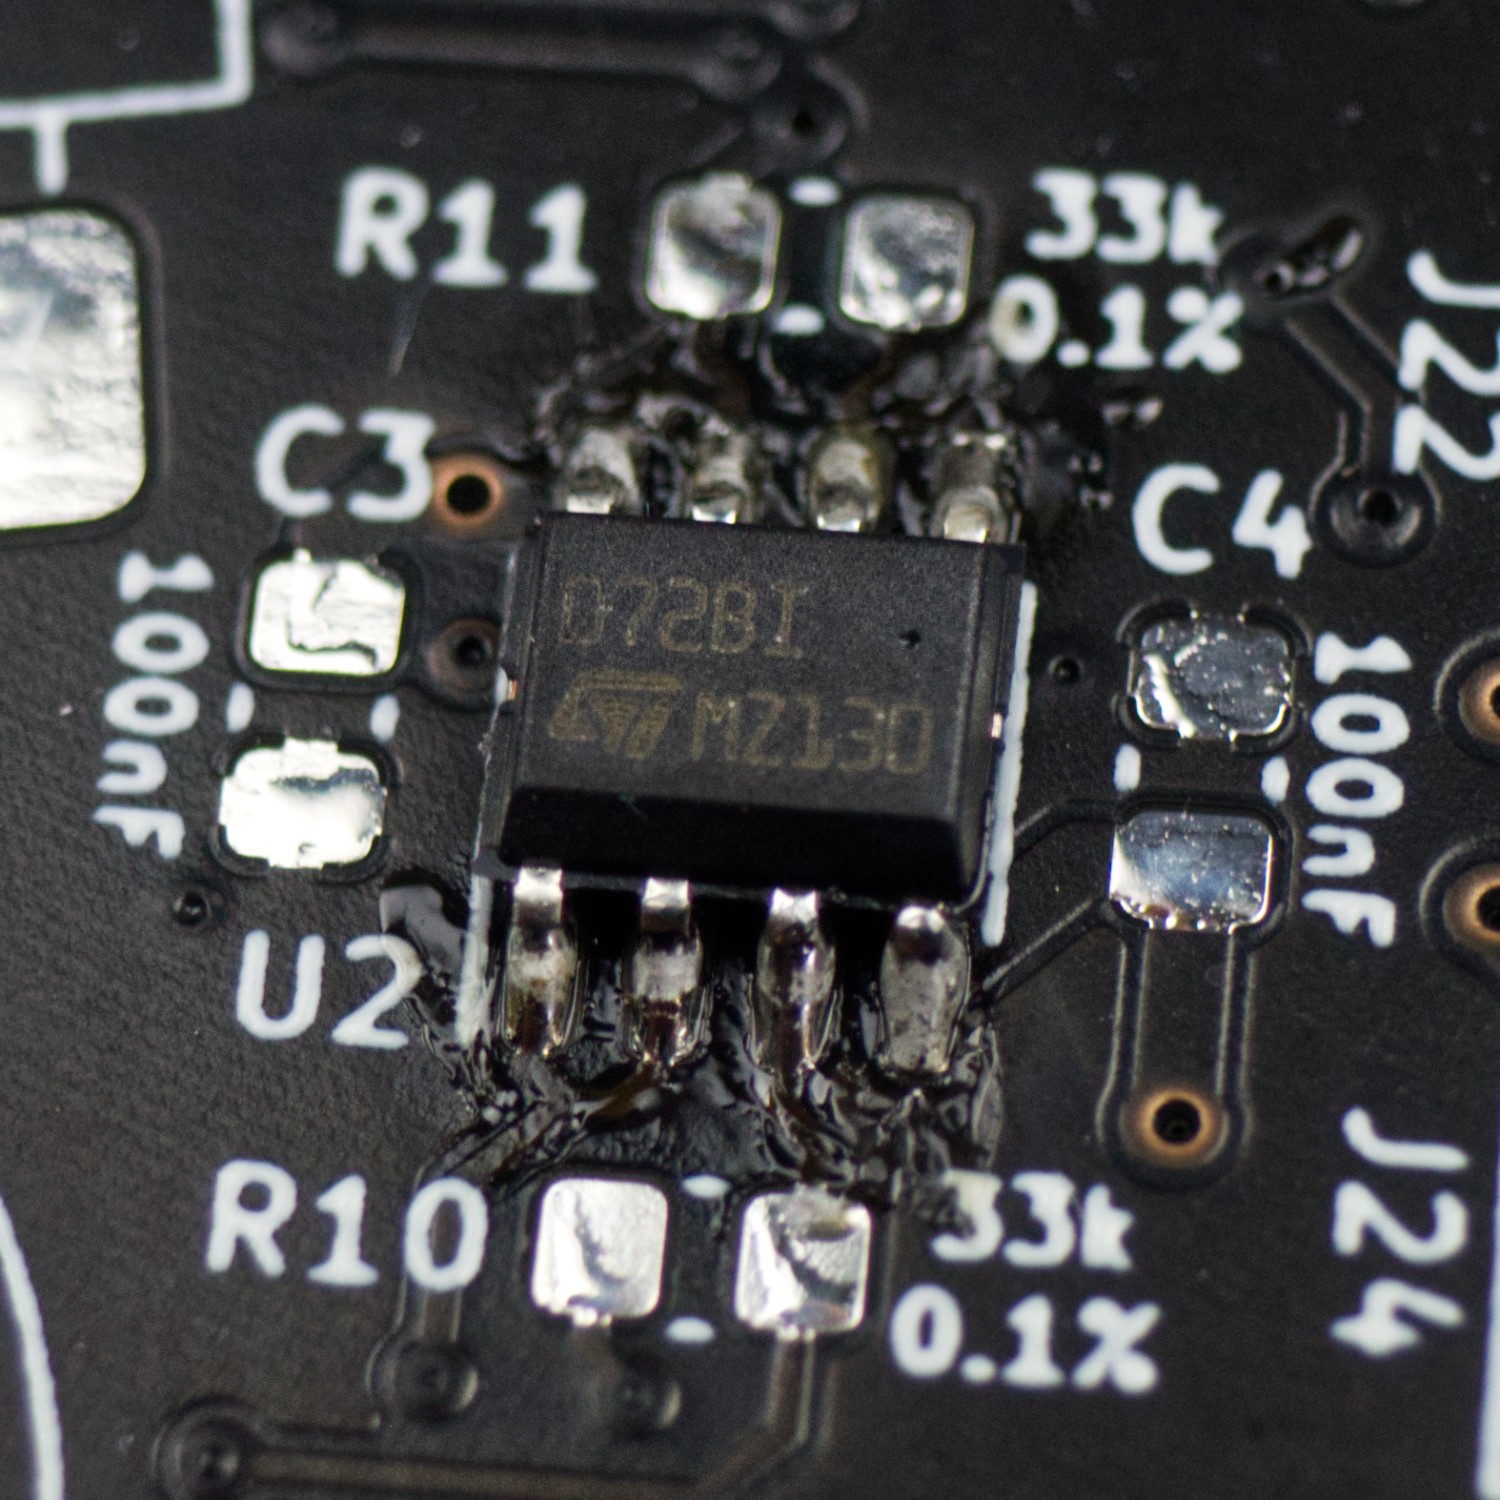
\includegraphics[width=46mm]{images/section_1-4_opamp.jpg}
    \hspace{2mm}
    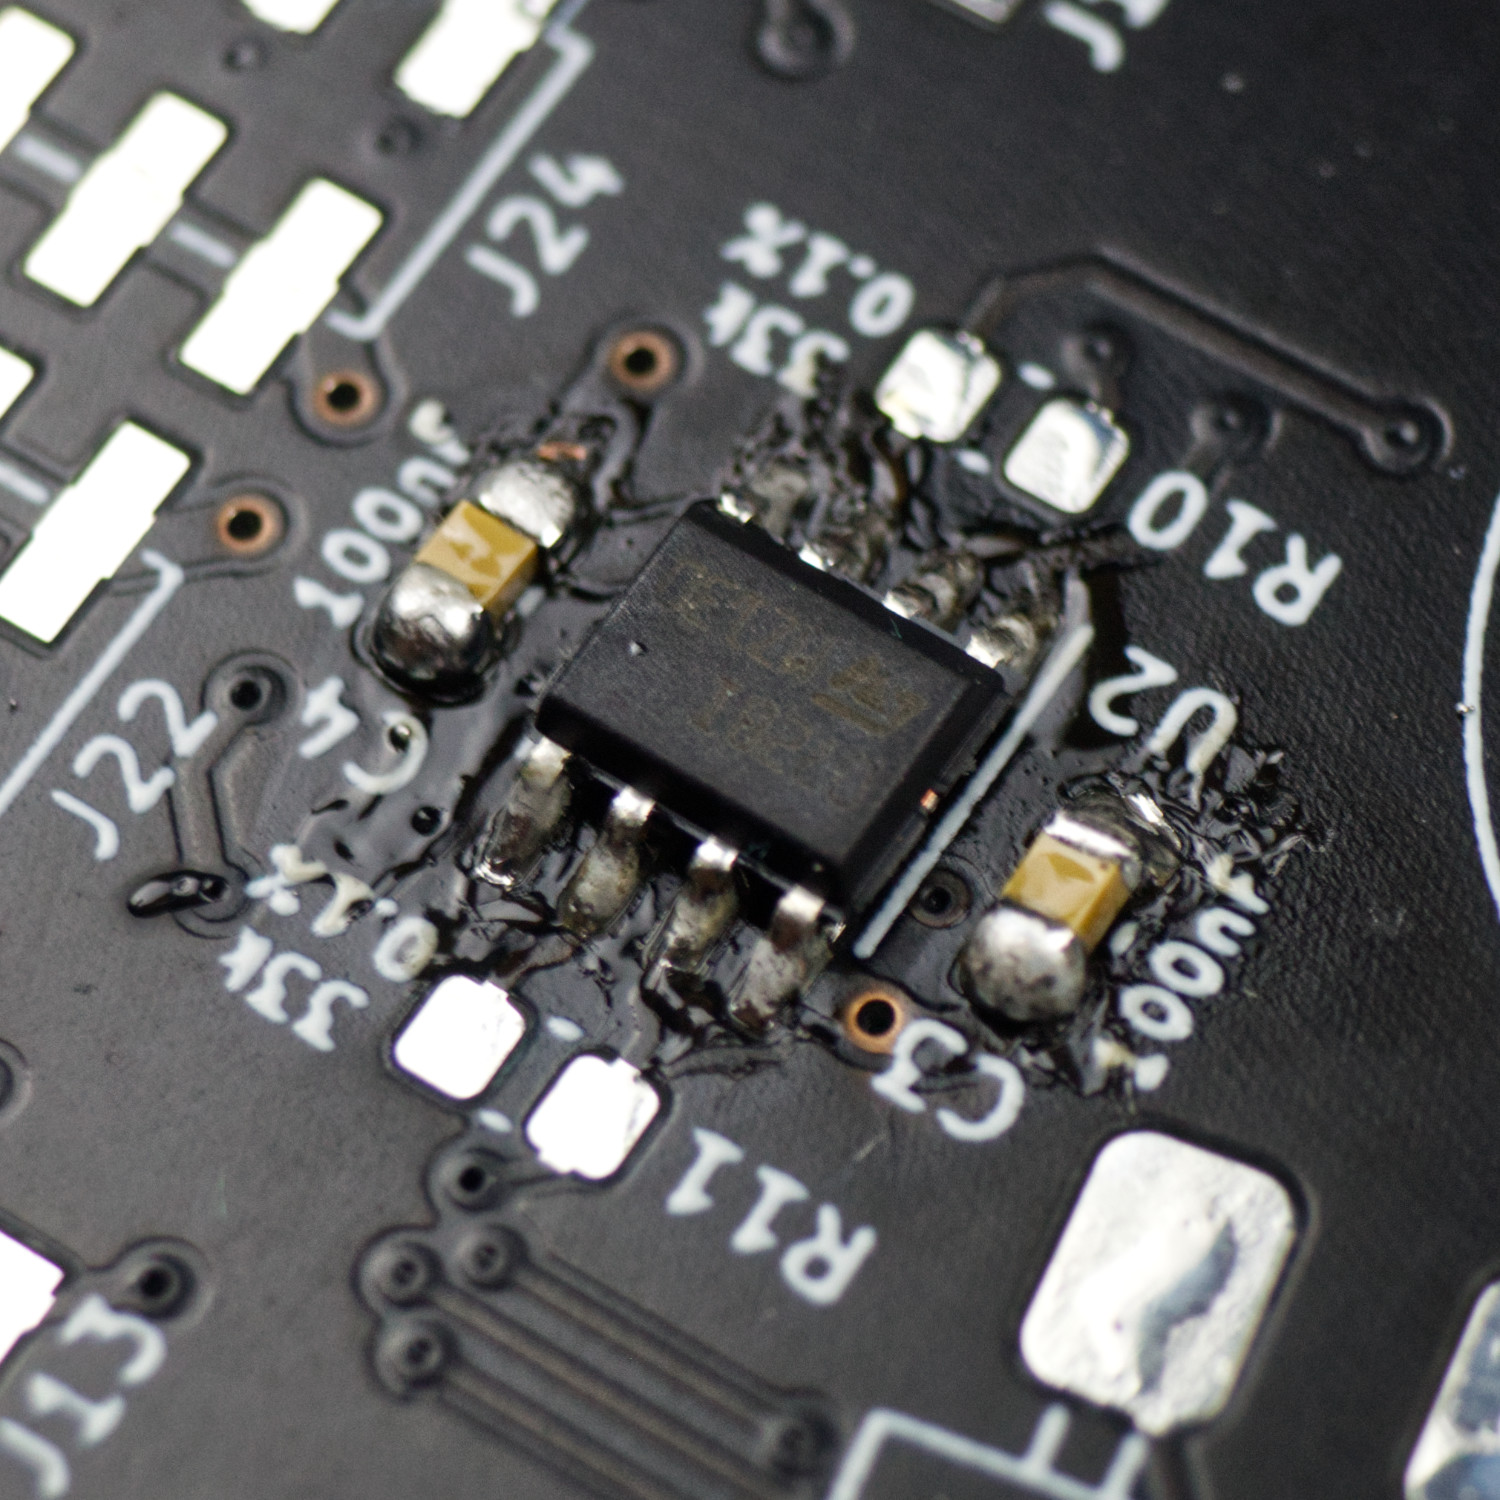
\includegraphics[width=46mm]{images/section_1-4_capacitors.jpg}
    \hspace{2mm}
    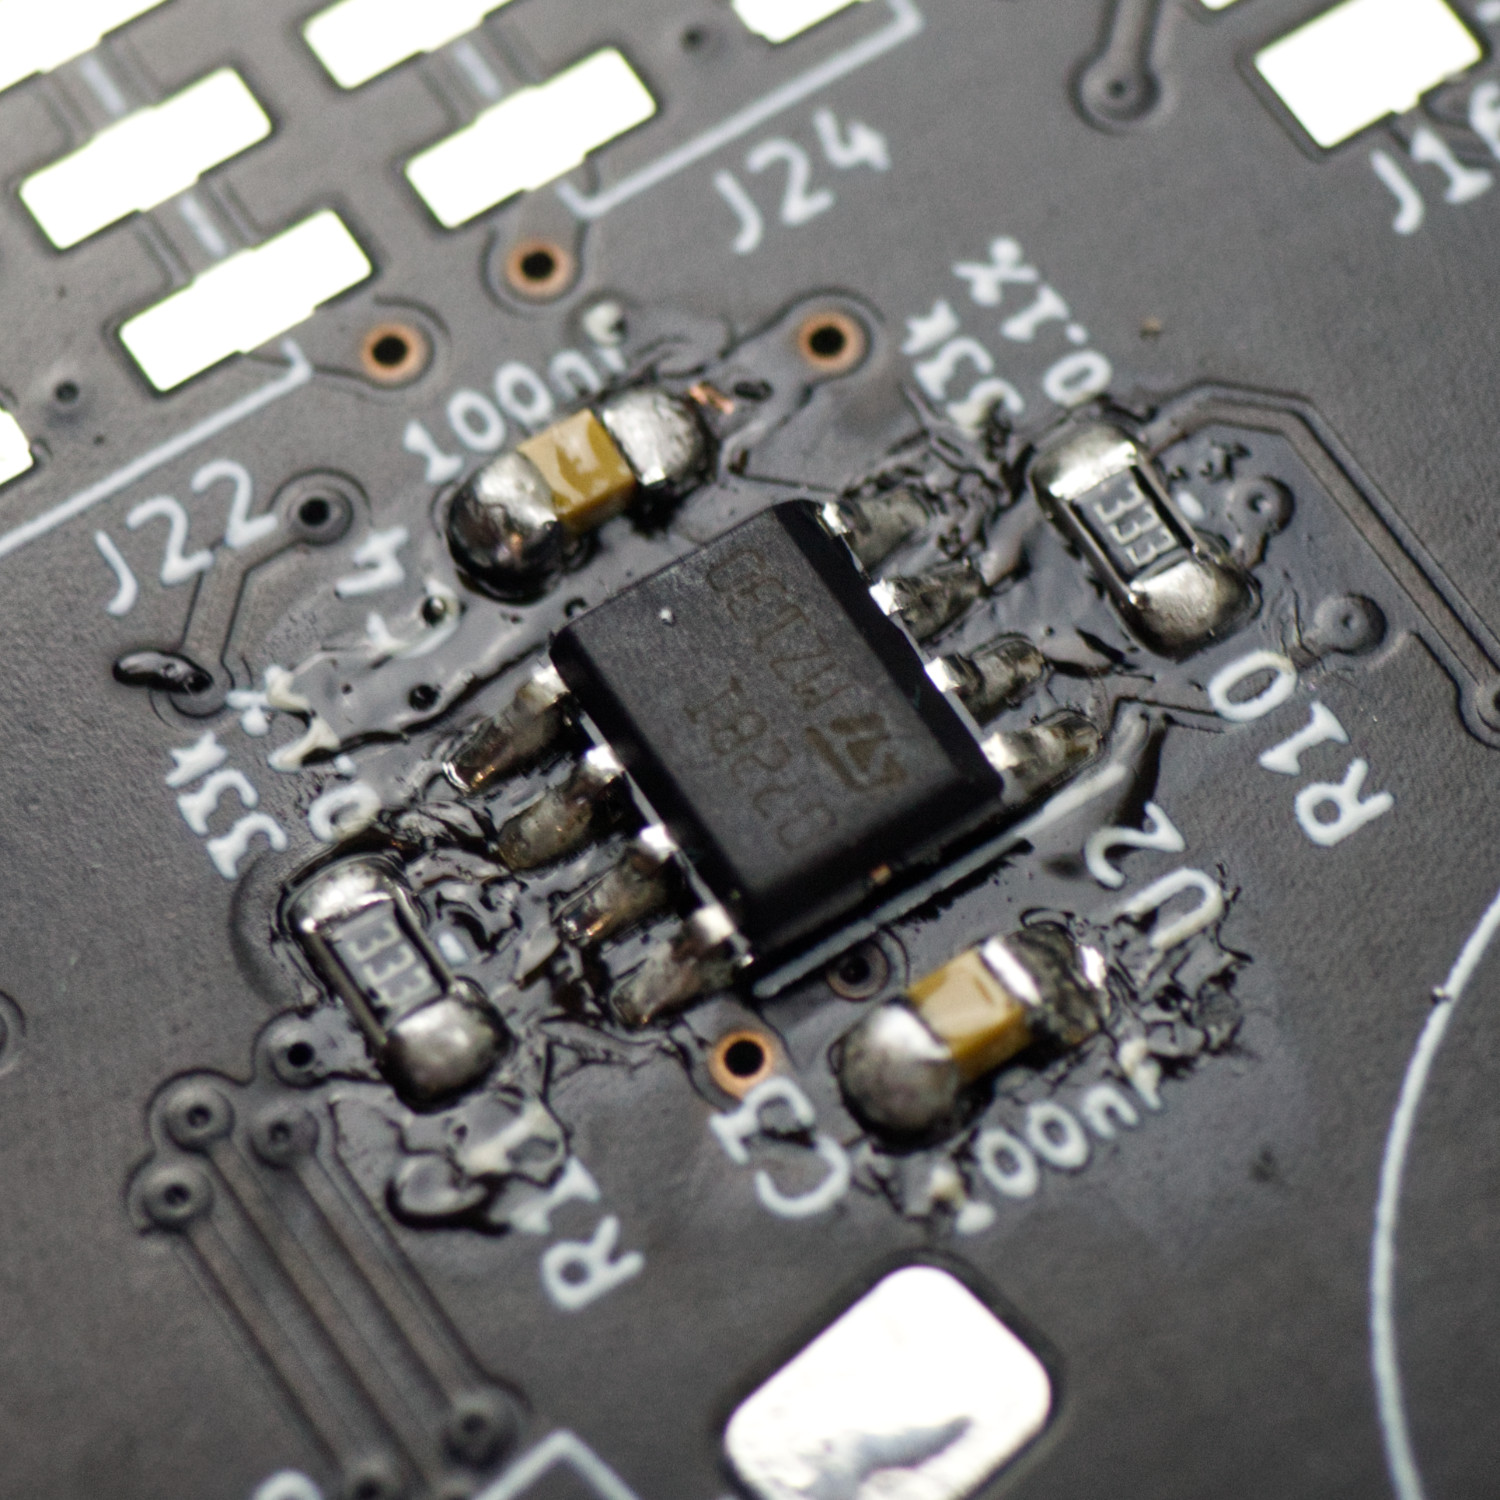
\includegraphics[width=46mm]{images/section_1-4_resistors.jpg}
\end{figure}

\subsection{L78Lxx Voltage Reference}

\begin{center}
    \small
    \setlength\extrarowheight{8pt}
    \begin{tabularx}{\textwidth}{|c|c|c|X|l|l|}
        \hline\rowcolor{lightgray} & ID & Qty & Description & Code on Part & PCB Identifier\\
        \hline\checkbox{ea} & 14 & 1 & L78L05 Voltage Regulator, SOT-89 & TODO & U4\\
        \hline\checkbox{eb} & 16 & 1 & \makebox[2.8em]{\hfill 100nF} Capacitor, 0805 & - & C10\\
        \hline\checkbox{ec} & 17 & 1 & \makebox[2.8em]{\hfill 330nF} Capacitor, 0805 & - & C9\\
        \hline
    \end{tabularx}
\end{center}

This is the first of two voltage references that come with the full DIY kit. It uses a cheap
78xx regulator to produce a stable but not terribly accurate voltage reference. The particular
regulator that comes with the kit is a 5V one, but ones for other voltages are also available.

The output voltage of the voltage reference gets buffered by one channel of the
\hyperref[sec:reference_voltage_buffer]{Reference Voltage Buffer}, while the other one inverts
it to get the negative reference voltage. The buffering/inverting is not necessary per se, but
for this use case, the OpAmp offers some protection against damaging the references directly
by connecting something in the wrong way. Using a low-offset OpAmp in combination with 0.1\%
precision resistors, is also almost always more cost-effective than adding a separate negative
reference.

Start with the L78L05 regulator. Solder the outer pins first, then the center pin and the tab
(these can take a while to solder because of their large thermal mass).

Then, assemble the 330nF input and 100nF output capacitors.

\begin{figure}[H]
    \centering
    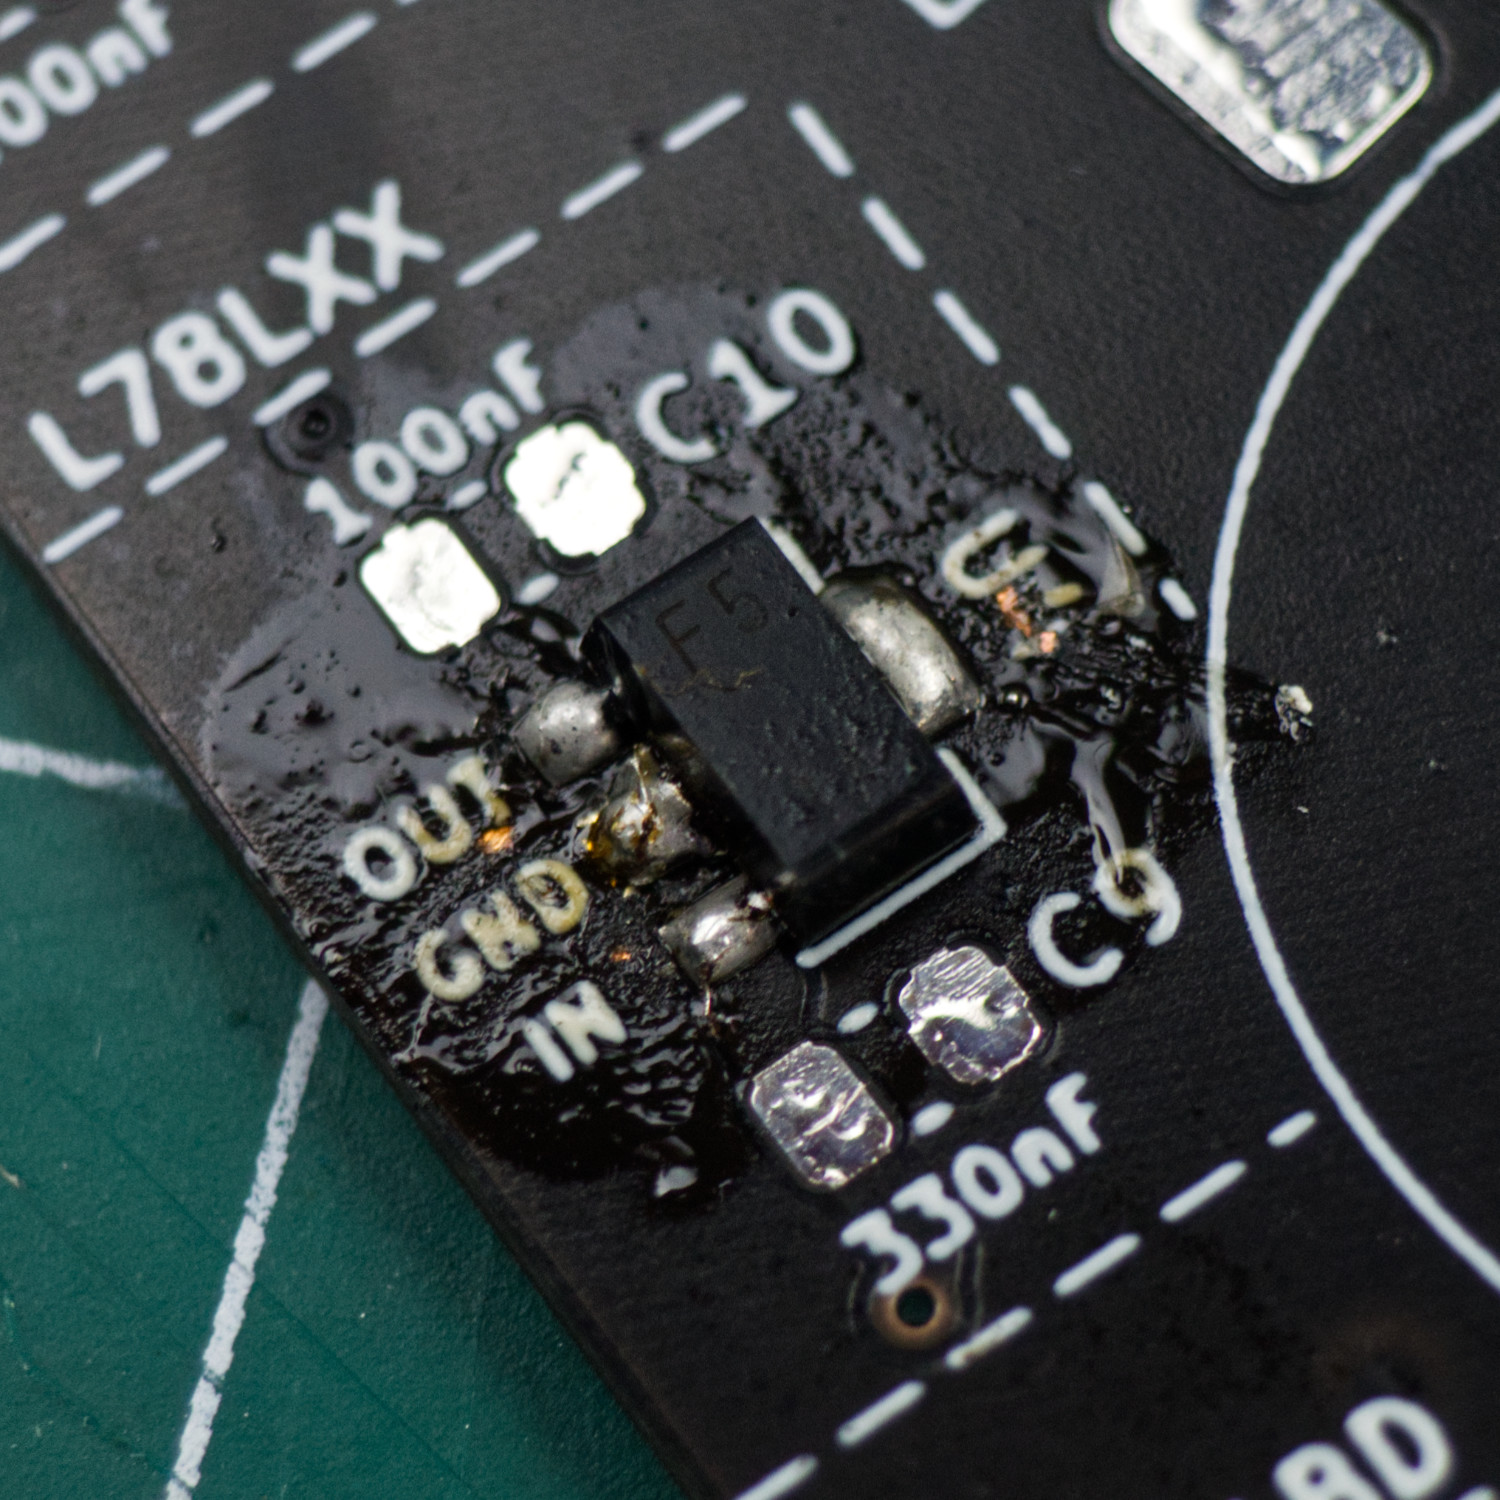
\includegraphics[width=46mm]{images/section_1-5_regulator.jpg}
    \hspace{2mm}
    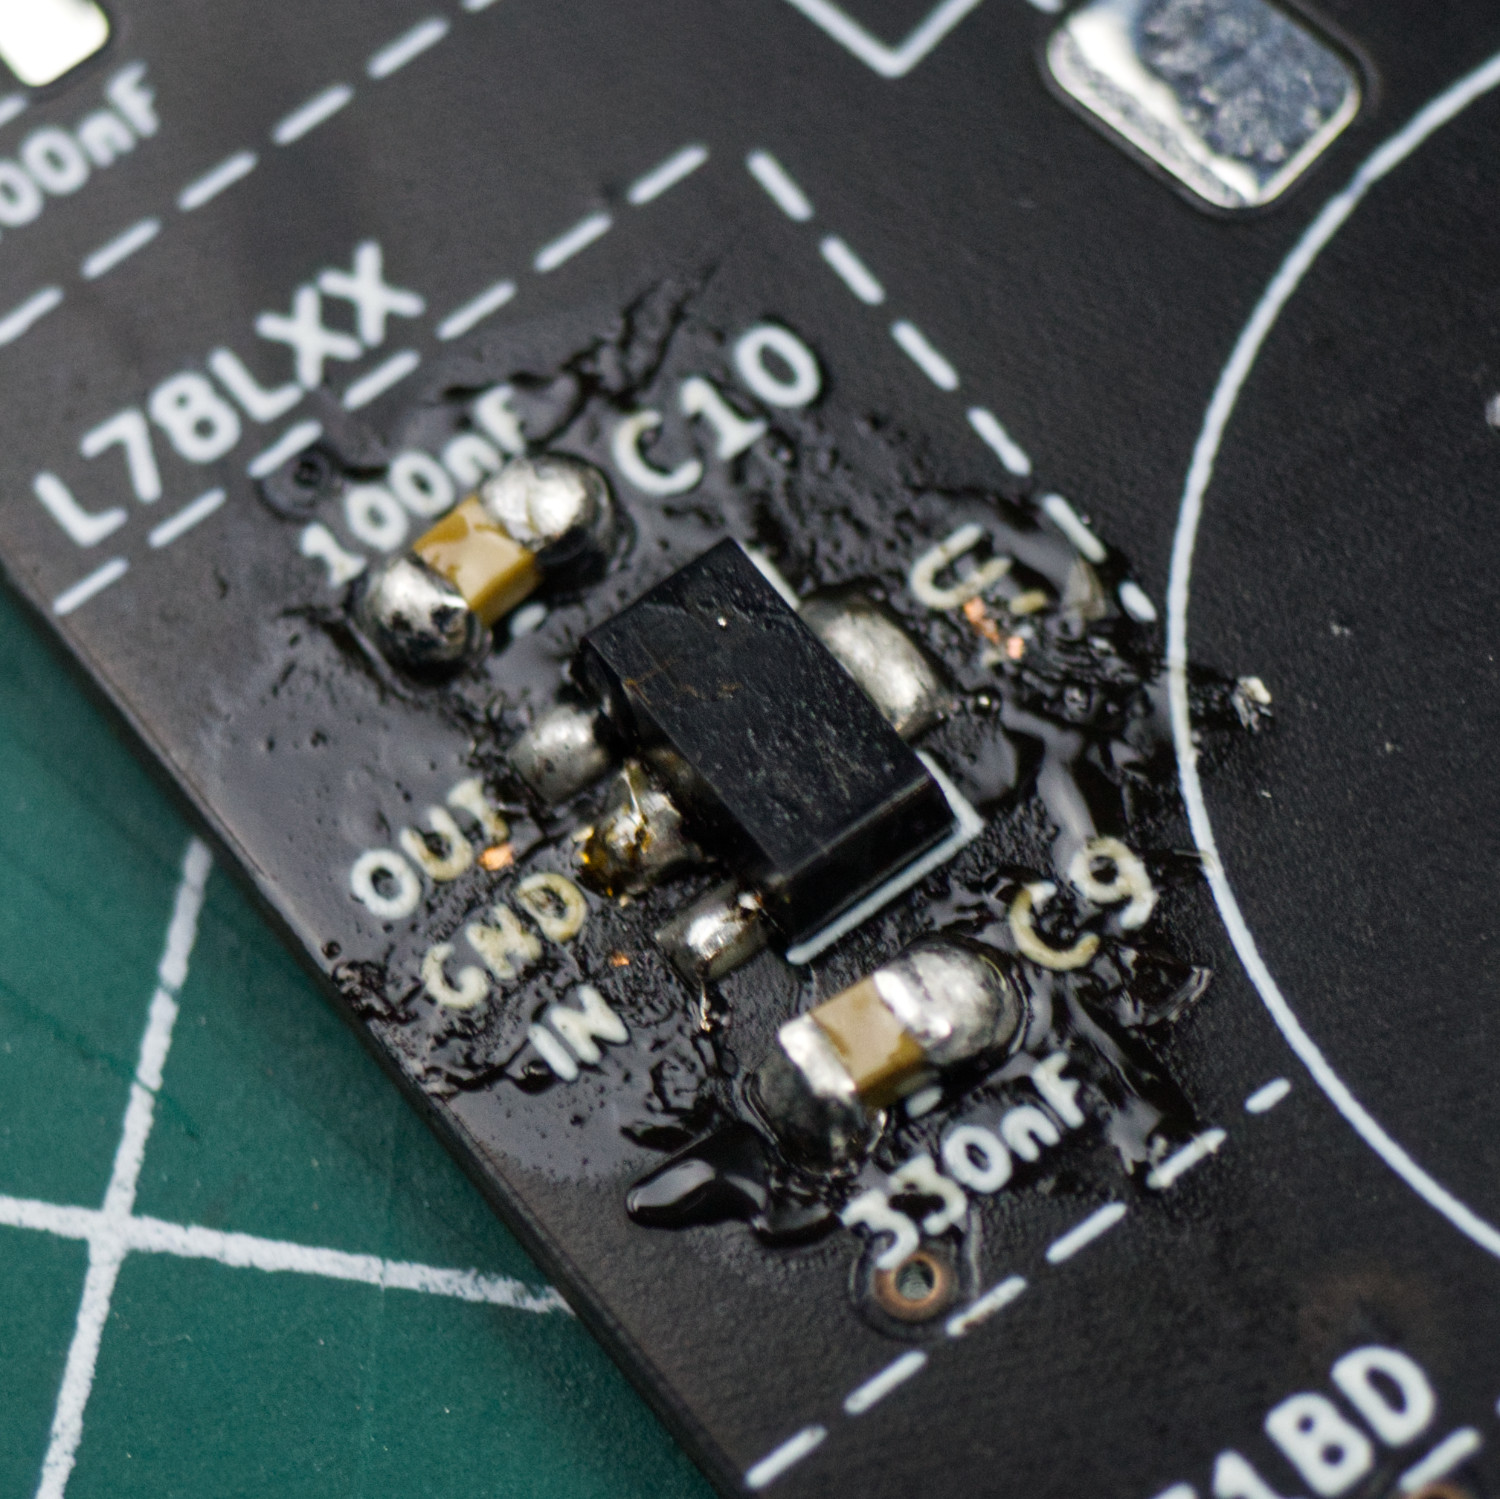
\includegraphics[width=46mm]{images/section_1-5_capacitors.jpg}
    \hspace{2mm}
    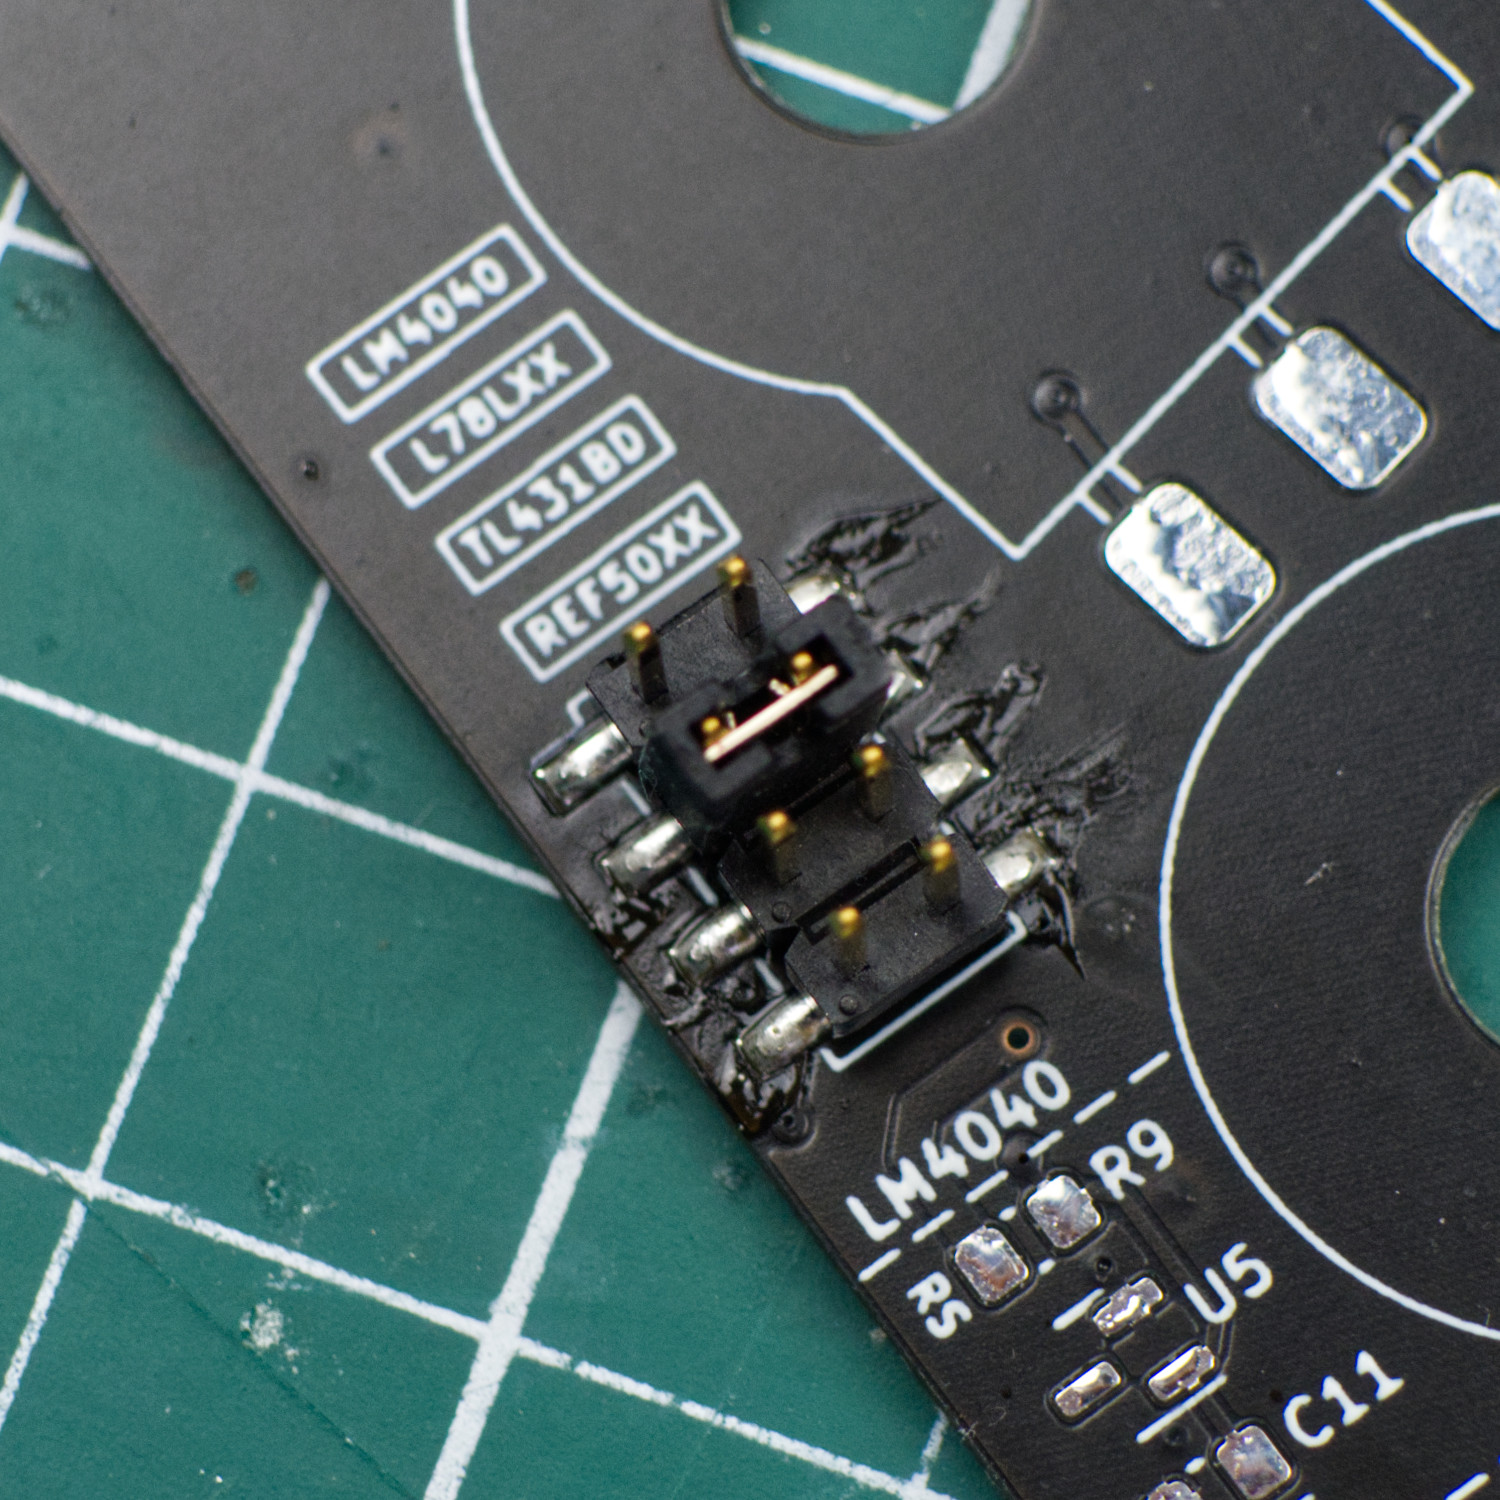
\includegraphics[width=46mm]{images/section_1-5_header.jpg}
\end{figure}

\subsection{LM4040 Voltage Reference}

\begin{center}
    \small
    \setlength\extrarowheight{8pt}
    \begin{tabularx}{\textwidth}{|c|c|c|X|l|l|}
        \hline\rowcolor{lightgray} & ID & Qty & Description & Code on Part & PCB Identifier\\
        \hline\checkbox{la} & 15 & 1 & LM4040 Voltage Reference, SOT-23 & TODO & U5\\
        \hline\checkbox{lb} &  7 & 1 & 10k Resistor, 0805 1\% & TODO & R9\\
        \hline\checkbox{lc} & 16 & 1 & 100nF Capacitor, 0805 & - & C11\\
        \hline\checkbox{ld} &  2 & 1 & 2×4 Header & - & J18\\
        \hline\checkbox{le} &  3 & 1 & Jumper & - & -\\
        \hline
    \end{tabularx}
\end{center}

This is the second voltage reference that come with the full DIY kit. It uses a LM4040 Zener
reference to produce a very stable and accurate voltage reference. The LM4040 that comes with
the kit is a 2.5V, C-Grade variant with 0.5\% output Tolerance (other variants are available).

\textit{%
    Note: If you are using a LM4040 with a different reference Voltage, make sure to select
    an appropriate bias resistor, according to
    \hyperref[ssec:appendix_lm4040_selecting_bias_resistor]{Selecting the bias resistor}.
}

Start with the LM4040 reference, then solder the 100nF output capacitor and the 10k bias
resistor.

Finally, solder the 2×4 header and add the jumper to select either the L78Lxx or LM4040
reference.

If you are building a kit and do not have any of the parts for the other Voltage References,
skip straight to \hyperref[sec:breadboard_headers]{assembling the Breadboard Headers}.

\subsection{\smaller (extra) \enspace \larger TL431B Voltage Reference}

TODO

\subsection{\smaller (extra) \enspace \larger REF50xx Voltage Reference}

TODO

\pagebreak
\section{Breadboard Headers}
\label{sec:breadboard_headers}

\begin{figure}[H]
    \centering
    \begin{tikzpicture}
        \node[anchor=south west,inner sep=0] (image) at (0,0) {
            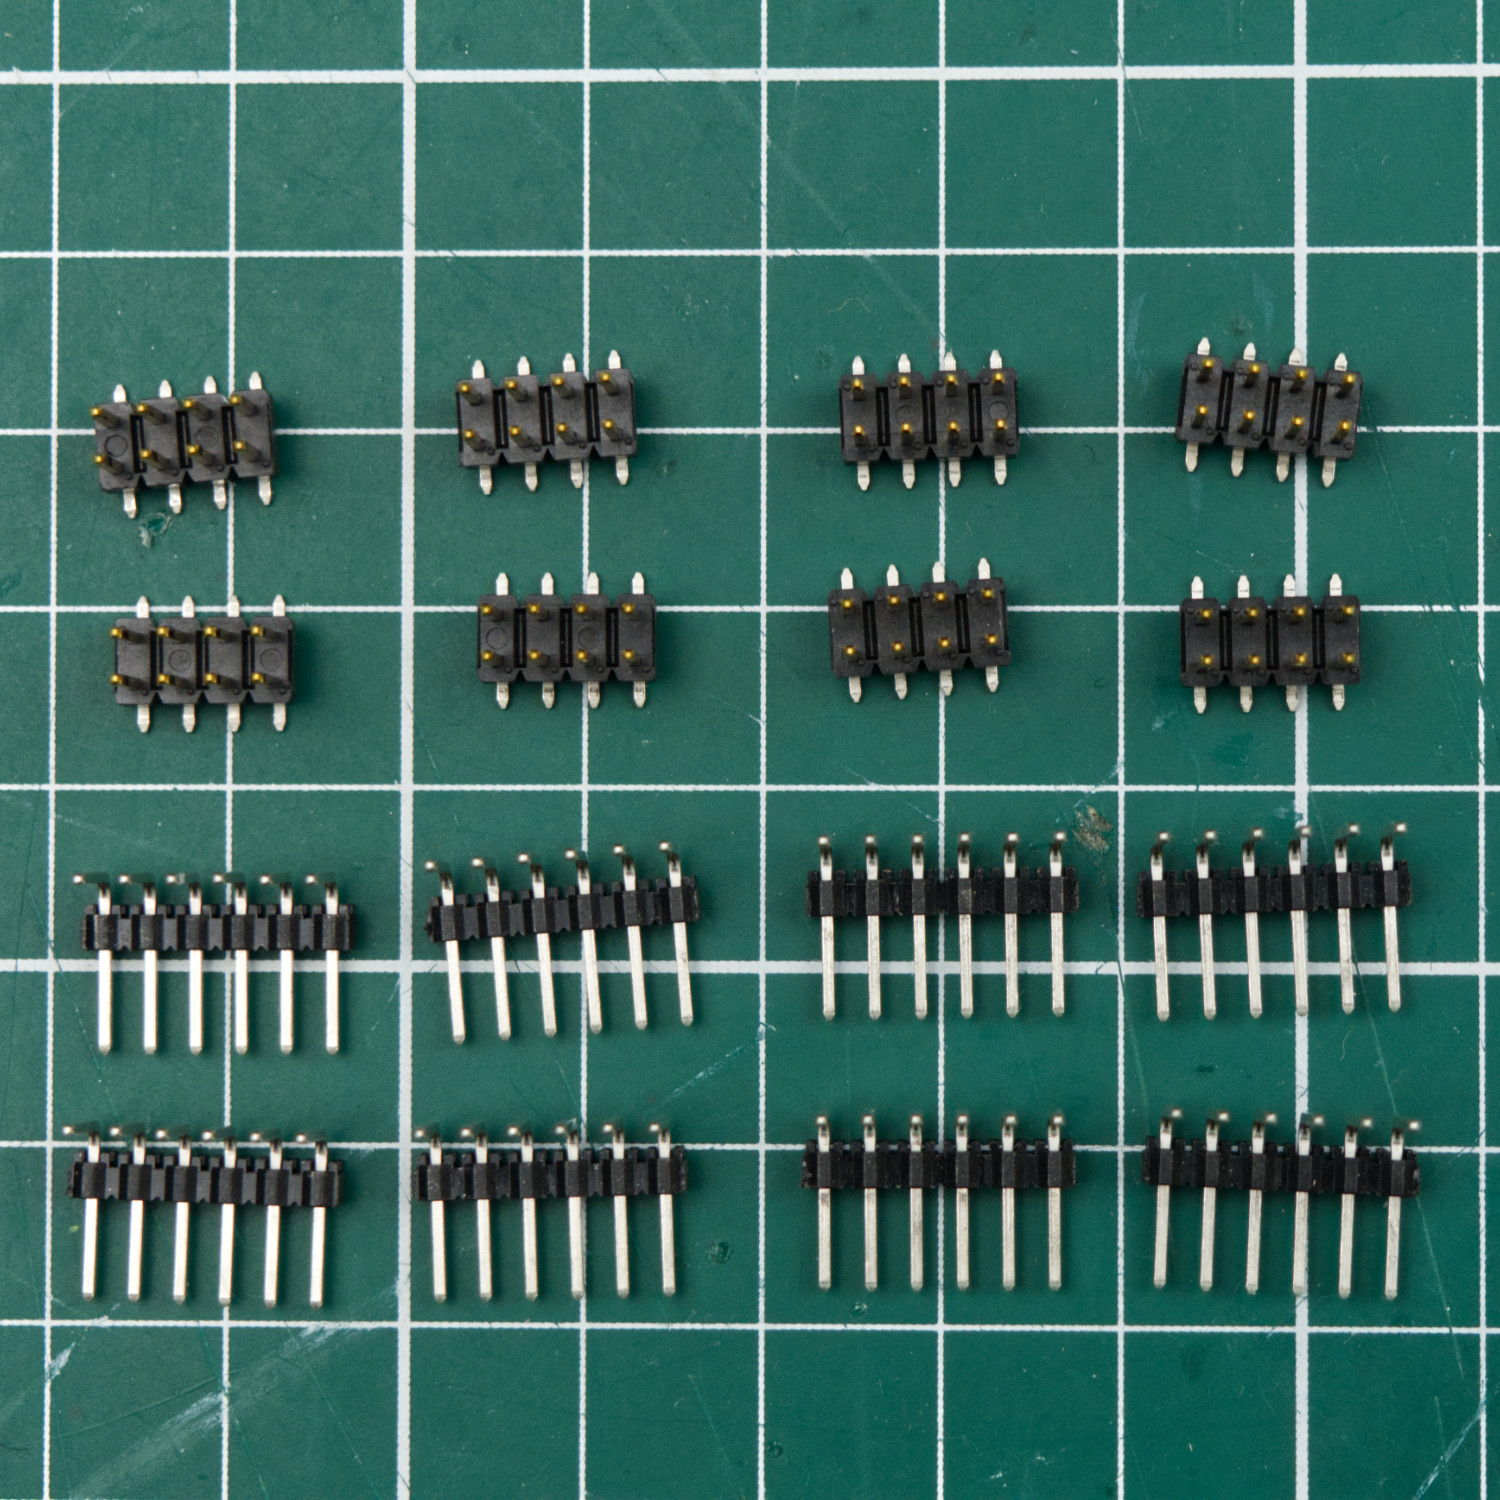
\includegraphics[width=7cm]{images/headers_topdown.jpg}
        };
        \begin{scope}[x={(image.south east)},y={(image.north west)}]
            \drawrect{0.03, 0.50}{0.97, 0.80} \drawtext{0.5, 0.75}{16}
            \drawrect{0.03, 0.10}{0.97, 0.48} \drawtext{0.5, 0.43}{17}
        \end{scope}
    \end{tikzpicture}
    \hspace{2mm}
    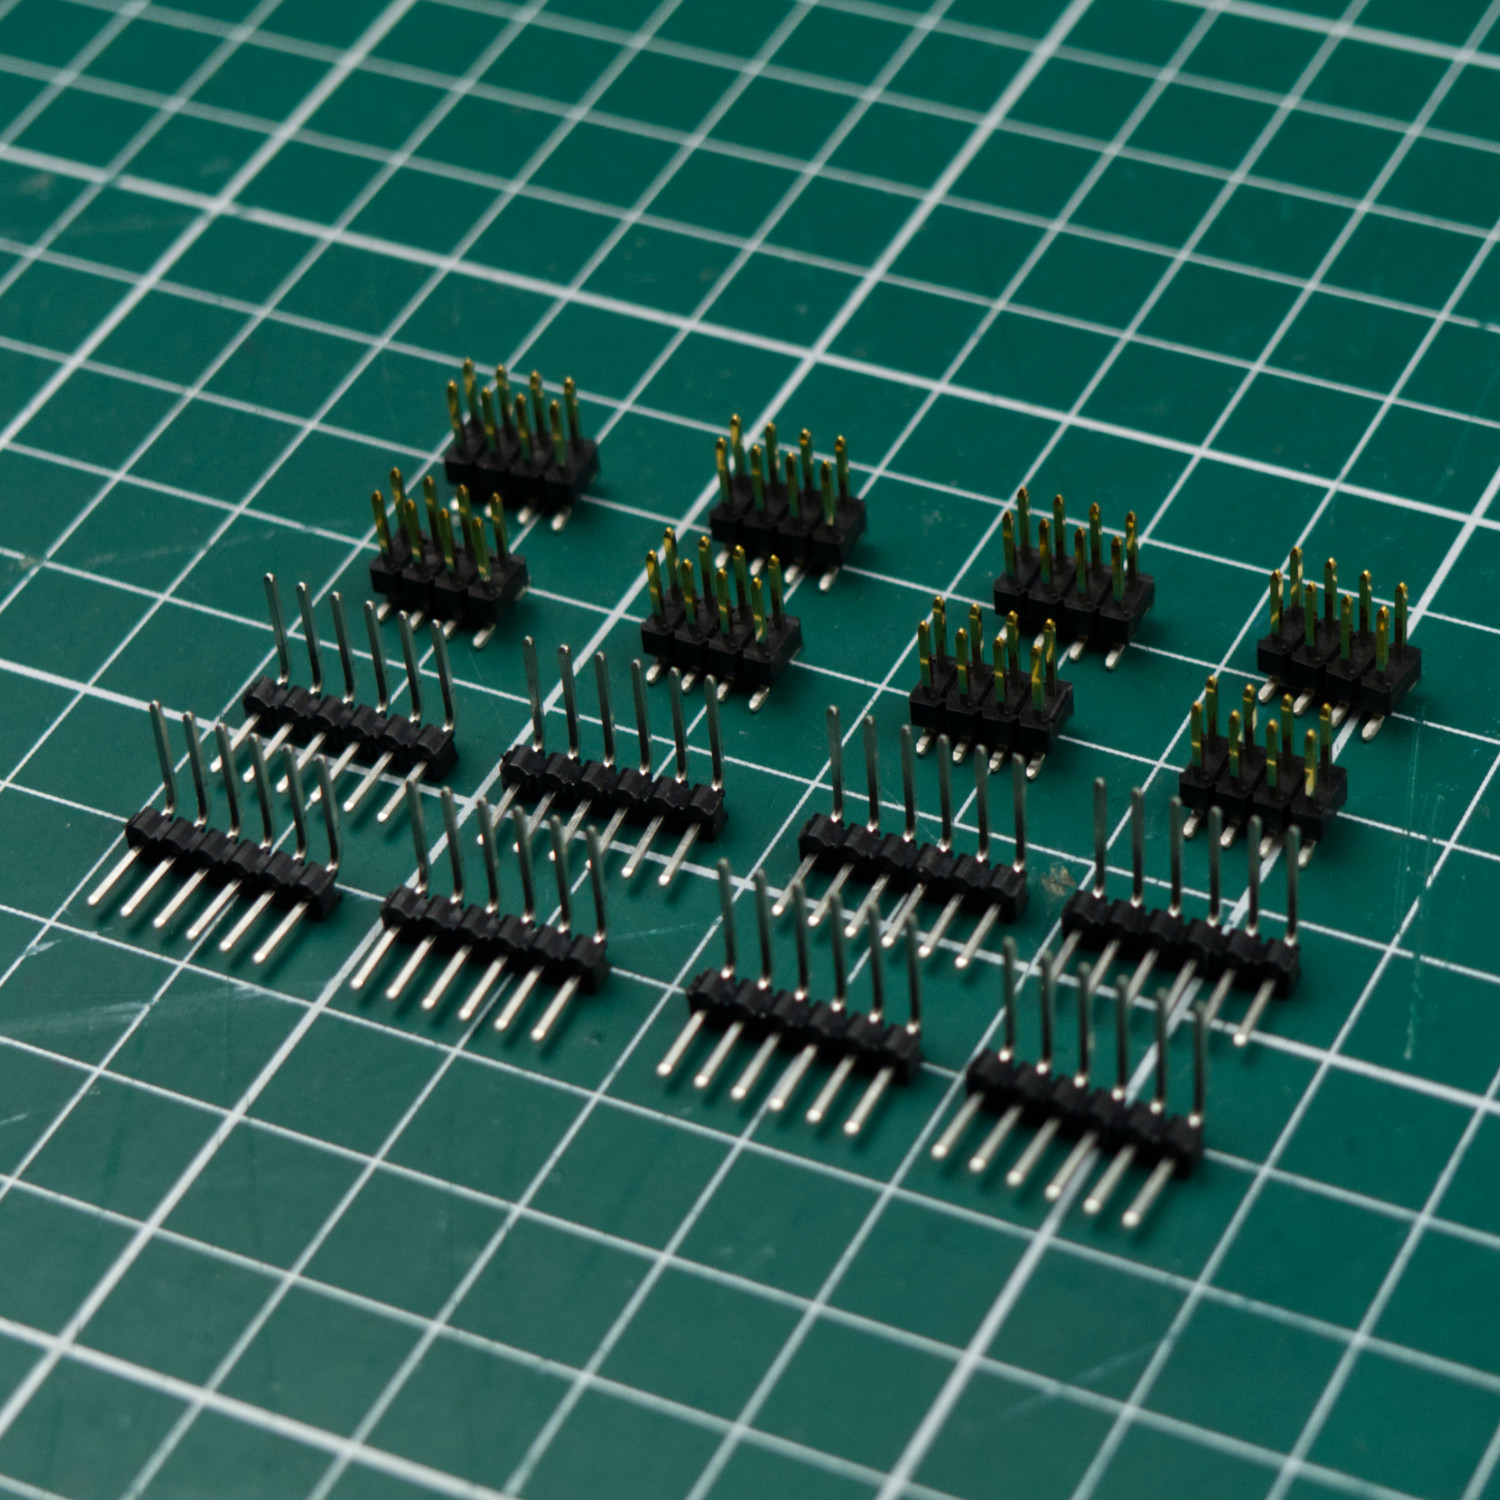
\includegraphics[width=7cm]{images/headers_side.jpg}
\end{figure}

\begin{center}
    \small
    \setlength\extrarowheight{4pt}
    \begin{tabularx}{\textwidth}{|c|c|X|l|}
        \hline \rowcolor{lightgray} ID & Qty & Description & PCB Identifier / Ref\\
        \hline 18 & 8 & 1×6 Right Angle Header & J10, J11, J12, J13, J14, J15, J16, J17\\
        \hline 19 & 8 & 2×4 Header & J19, J20, J21, J22, J23, J24, J25, J26\\
        \hline
    \end{tabularx}
\end{center}

\pagebreak

\subsection{Power Headers}

\begin{center}
    \small
    \setlength\extrarowheight{8pt}
    \begin{tabularx}{\textwidth}{|c|c|c|X|l|}
        \hline\rowcolor{lightgray} & ID & Qty & Description & PCB Identifier\\
        \hline\checkbox{fa} & 19 & 8 & 2×4 Header & J19, J20, J21, J22, J23, J24, J25, J26\\
        \hline
    \end{tabularx}
\end{center}

Take your time on soldering these, as they have to be aligned reasonably well, for the
breadboard to fit later on. It does not have to be perfect, but there should not be any obvious
rotations or offsets larger than \textasciitilde1mm.

To make this easier, tin one pin first (ideally, one that is not a ground pin), then solder the
header to it and center it to your best ability. After that, you can carefully push/bend it a
bit until the rotation looks good too, and solder the remaining pins.

The pins of the headers in the center can be tricky to solder, but you should still be able to
reach them, as shown. Be careful not to melt the plastic of the headers.

\begin{figure}[H]
    \centering
    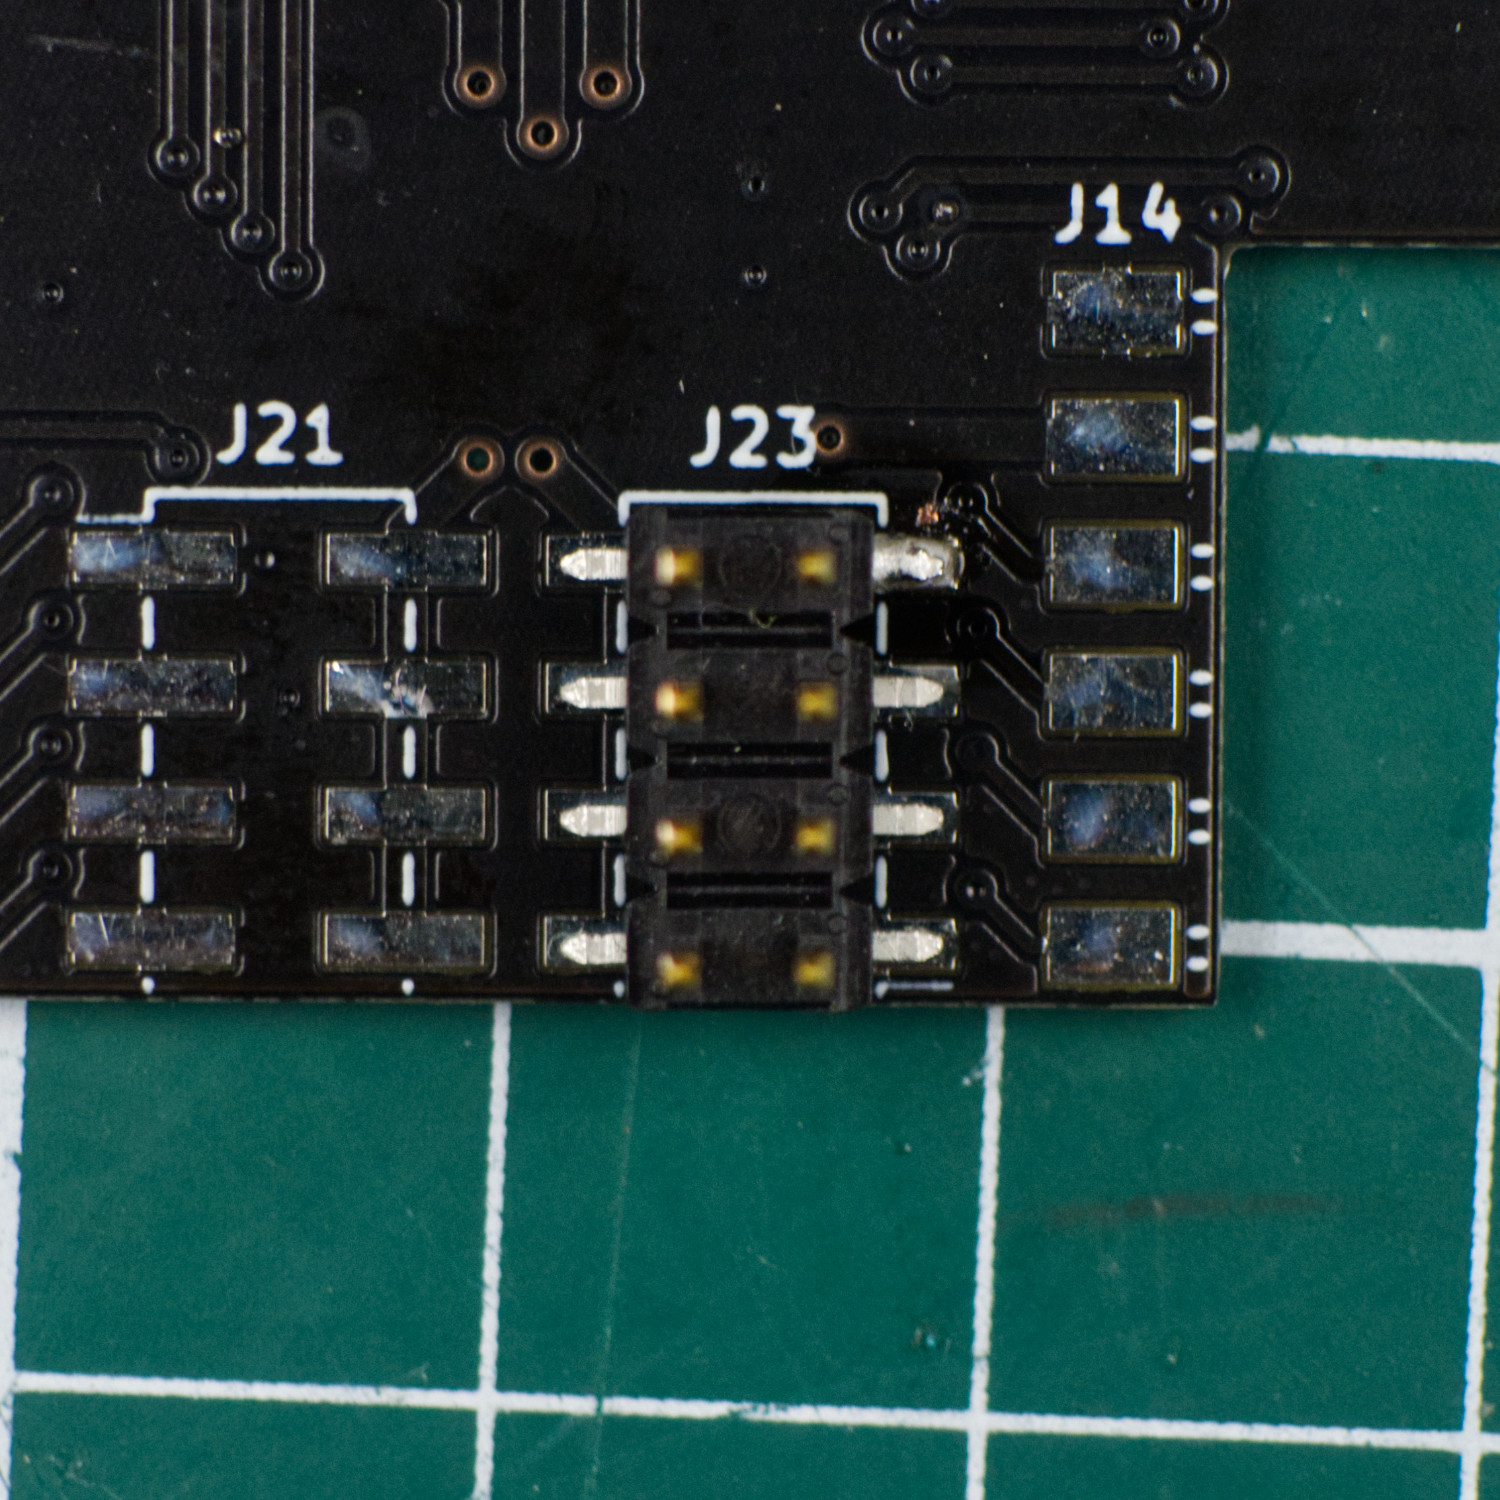
\includegraphics[width=46mm]{images/section_2-1_single.jpg}
    \hspace{2mm}
    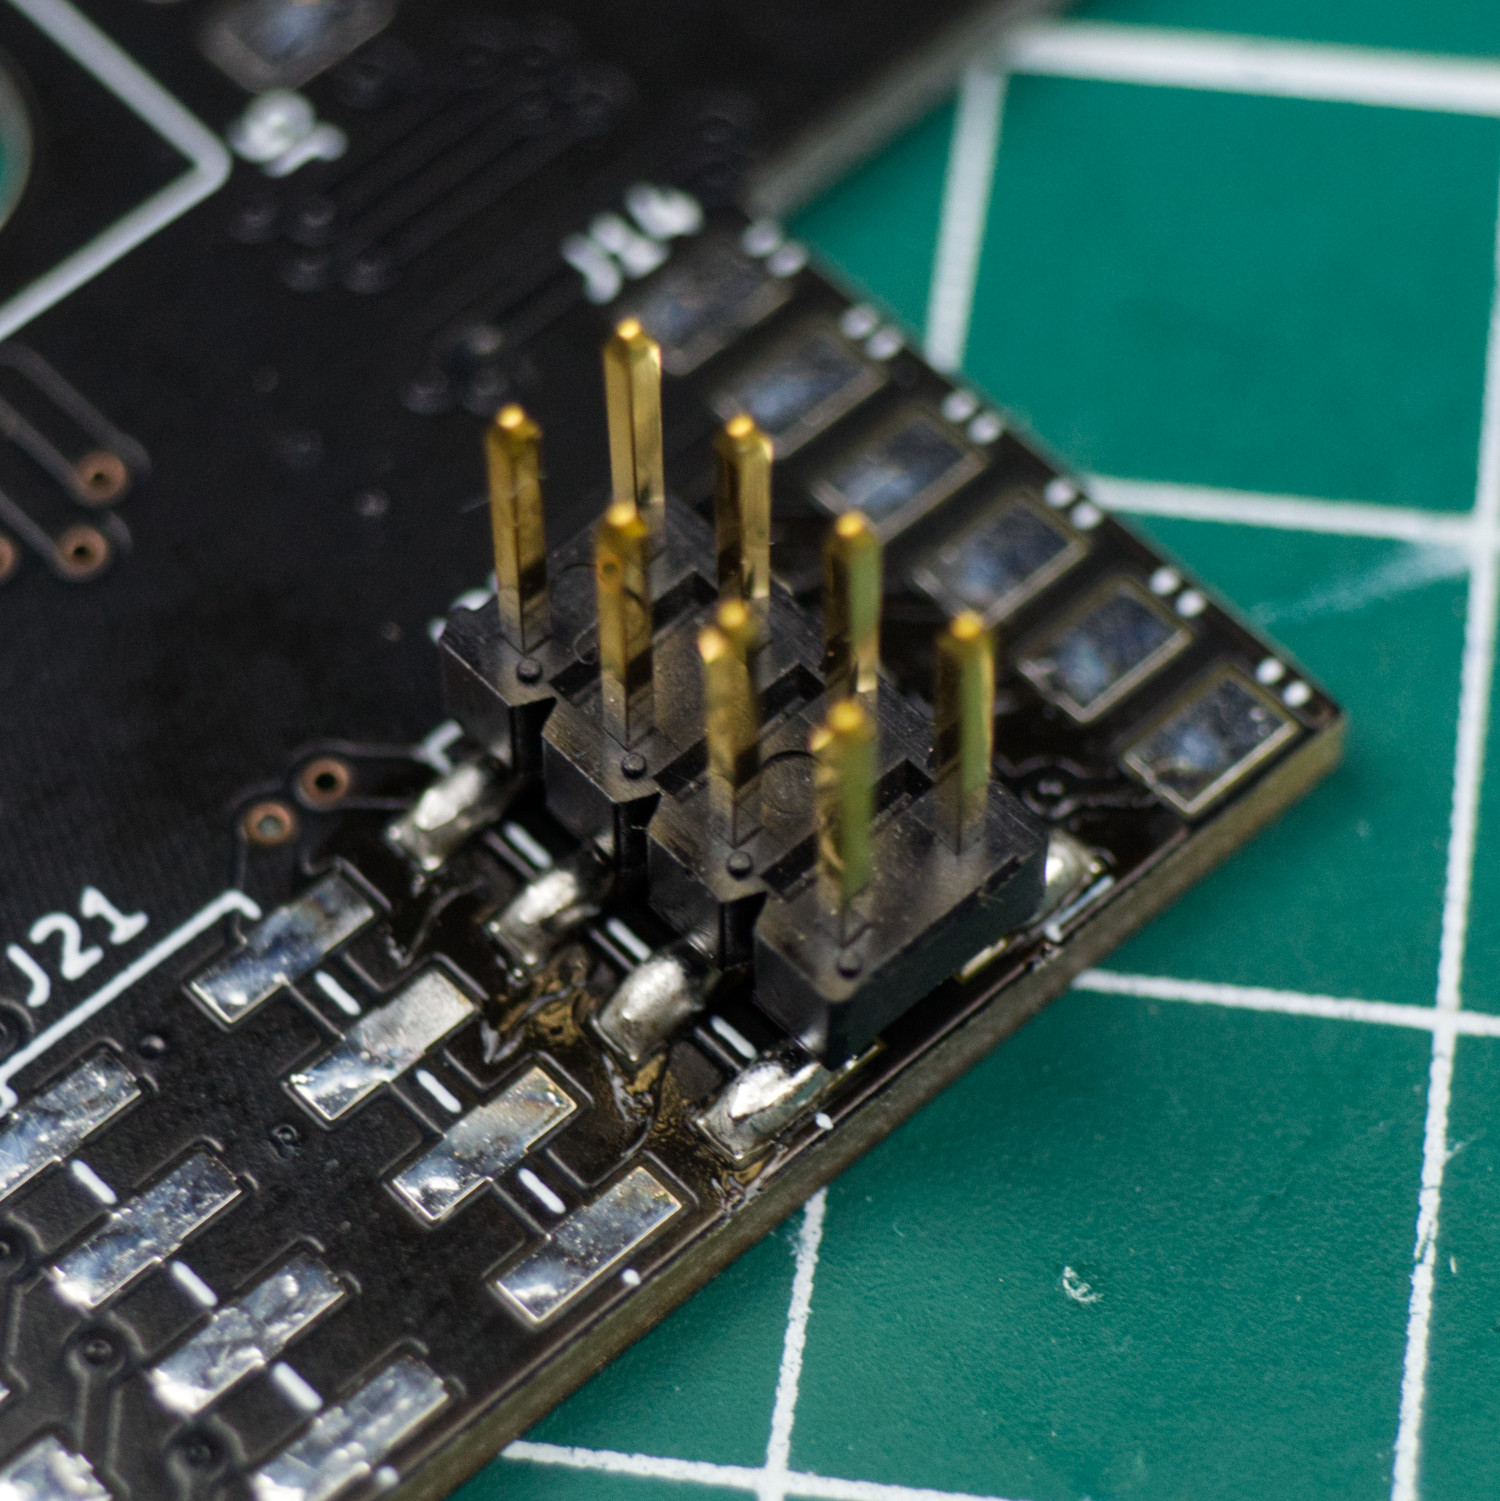
\includegraphics[width=46mm]{images/section_2-1_full.jpg}
    \hspace{2mm}
    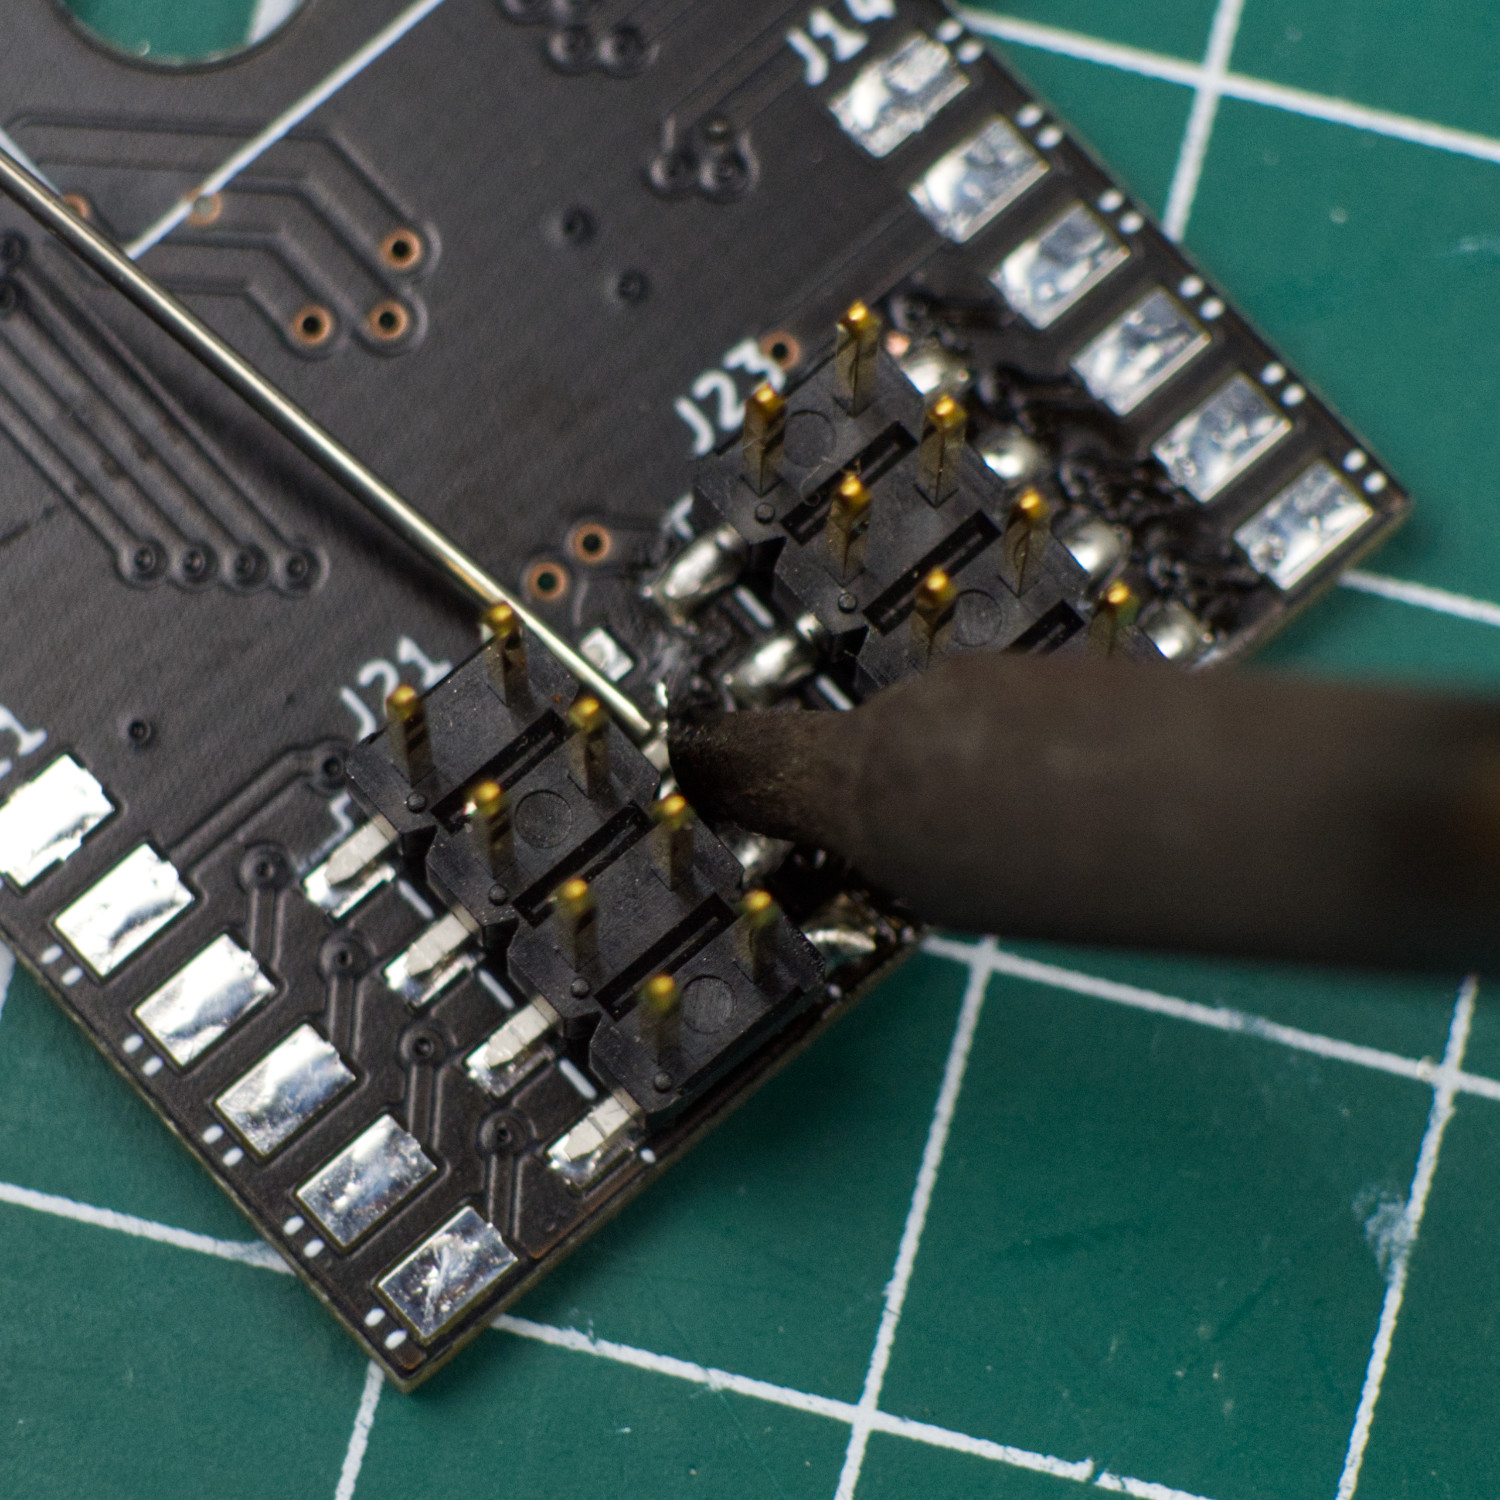
\includegraphics[width=46mm]{images/section_2-1_top.jpg}
\end{figure}

\subsection{Right Angle Headers}

\begin{center}
    \small
    \setlength\extrarowheight{8pt}
    \begin{tabularx}{\textwidth}{|c|c|c|X|l|}
        \hline\rowcolor{lightgray} & ID & Qty & Description & PCB Identifier\\
        \hline\checkbox{ga} & 18 & 8 & 1×6 Right Angle Header & J10, J11, J12, J13, J14, J15, J16, J17\\
        \hline
    \end{tabularx}
\end{center}

Take your side cutters and cut away about half (\textasciitilde3mm) of the shorter side of the
headers, so that when pushed into the corner of the PCB, as seen below, they do not interfere
with the power headers.

\begin{figure}[H]
    \centering
    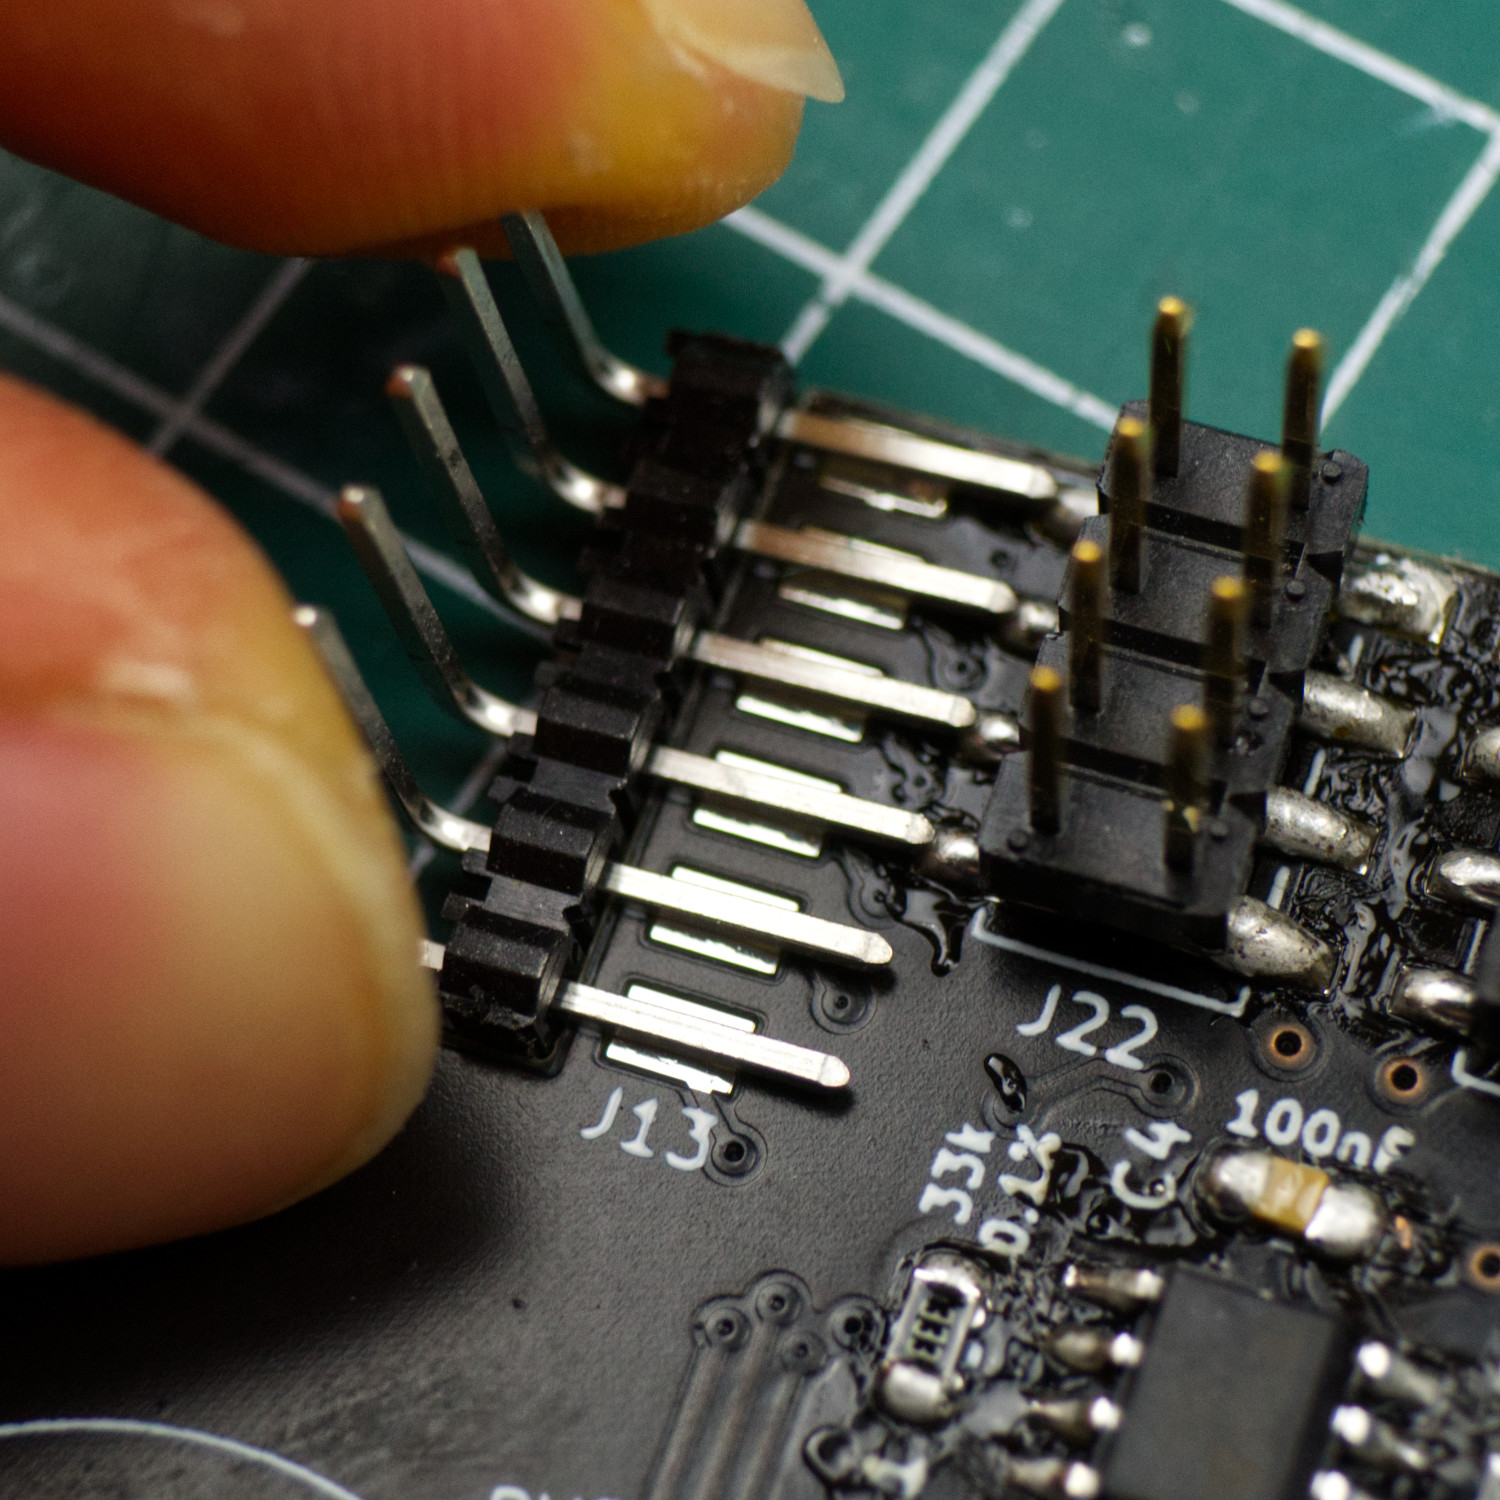
\includegraphics[width=46mm]{images/section_2-2_testfit.jpg}
    \hspace{2mm}
    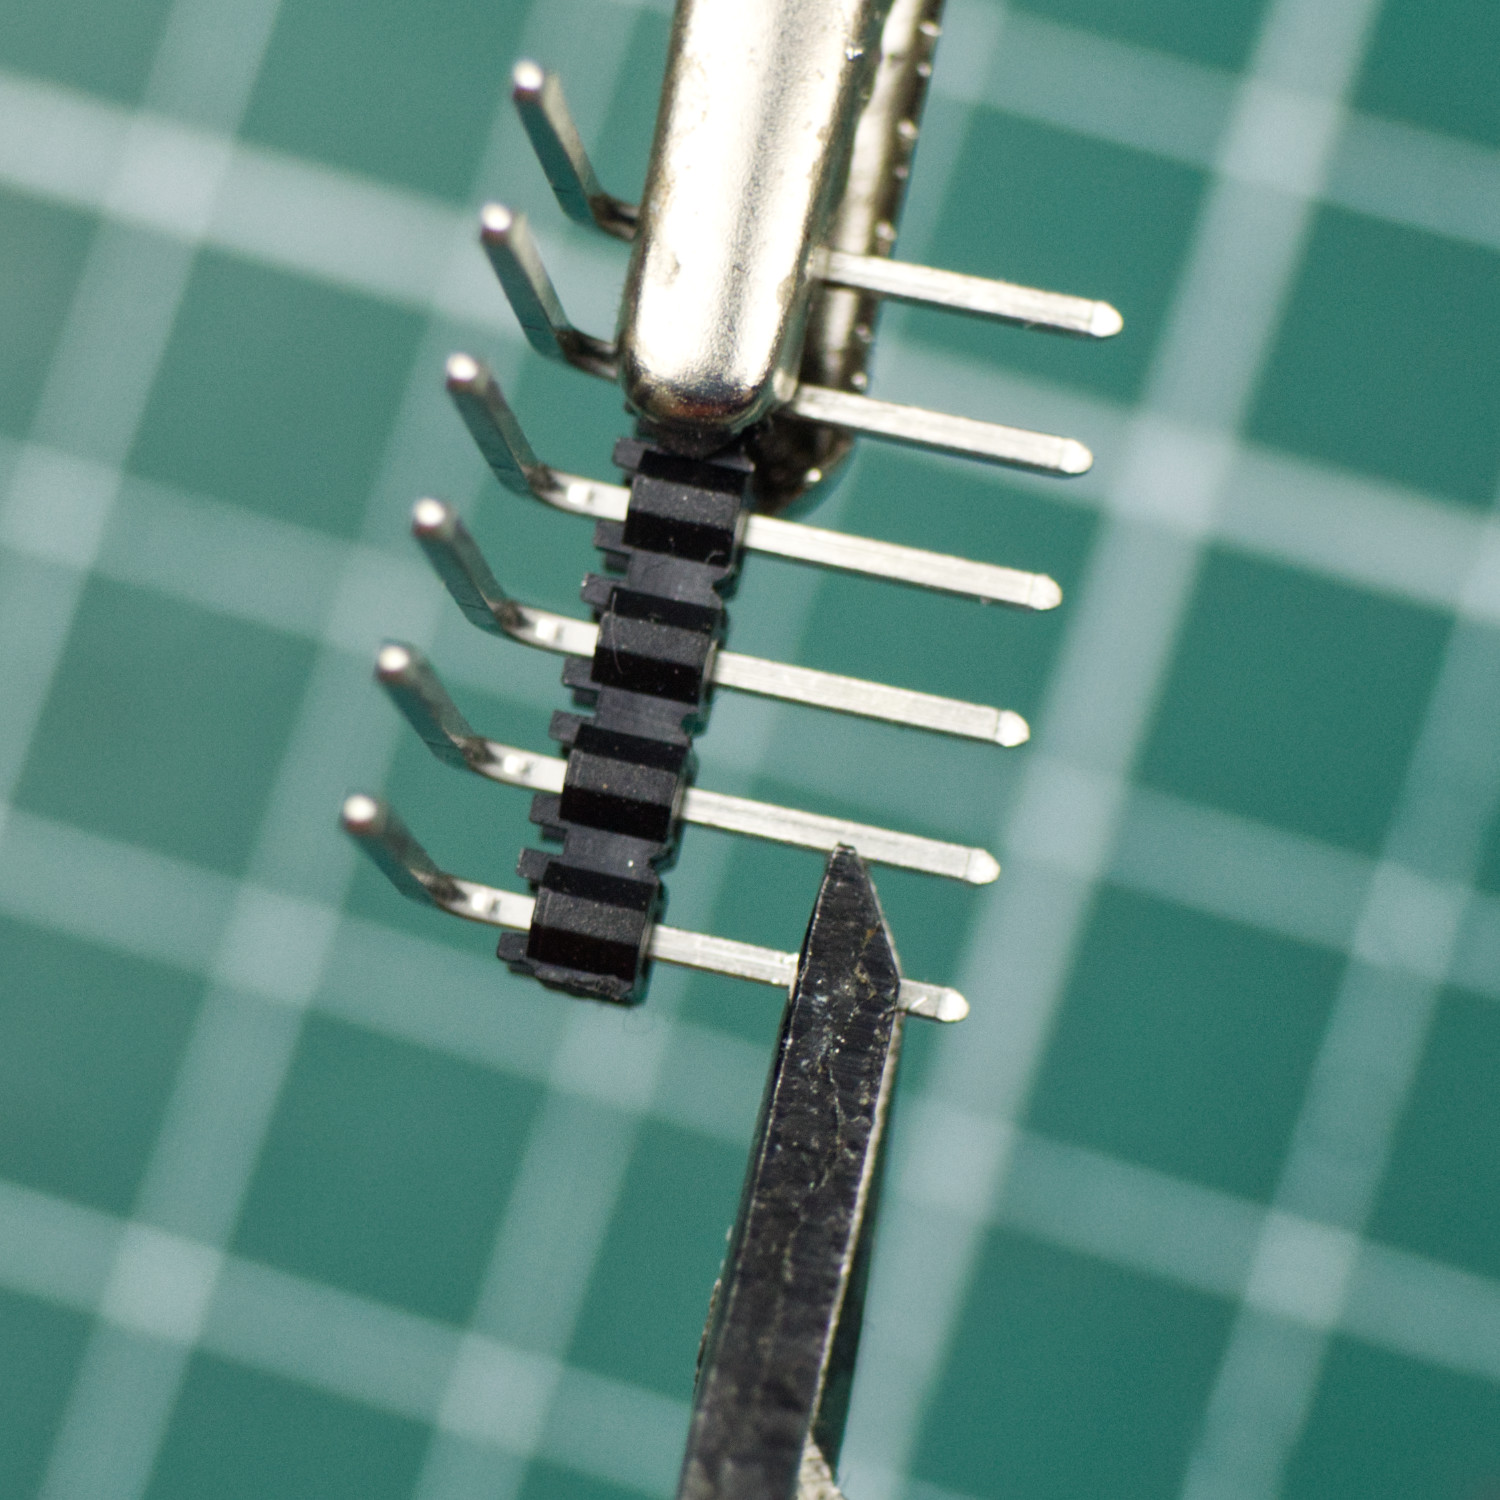
\includegraphics[width=46mm]{images/section_2-2_cutting.jpg}
    \hspace{2mm}
    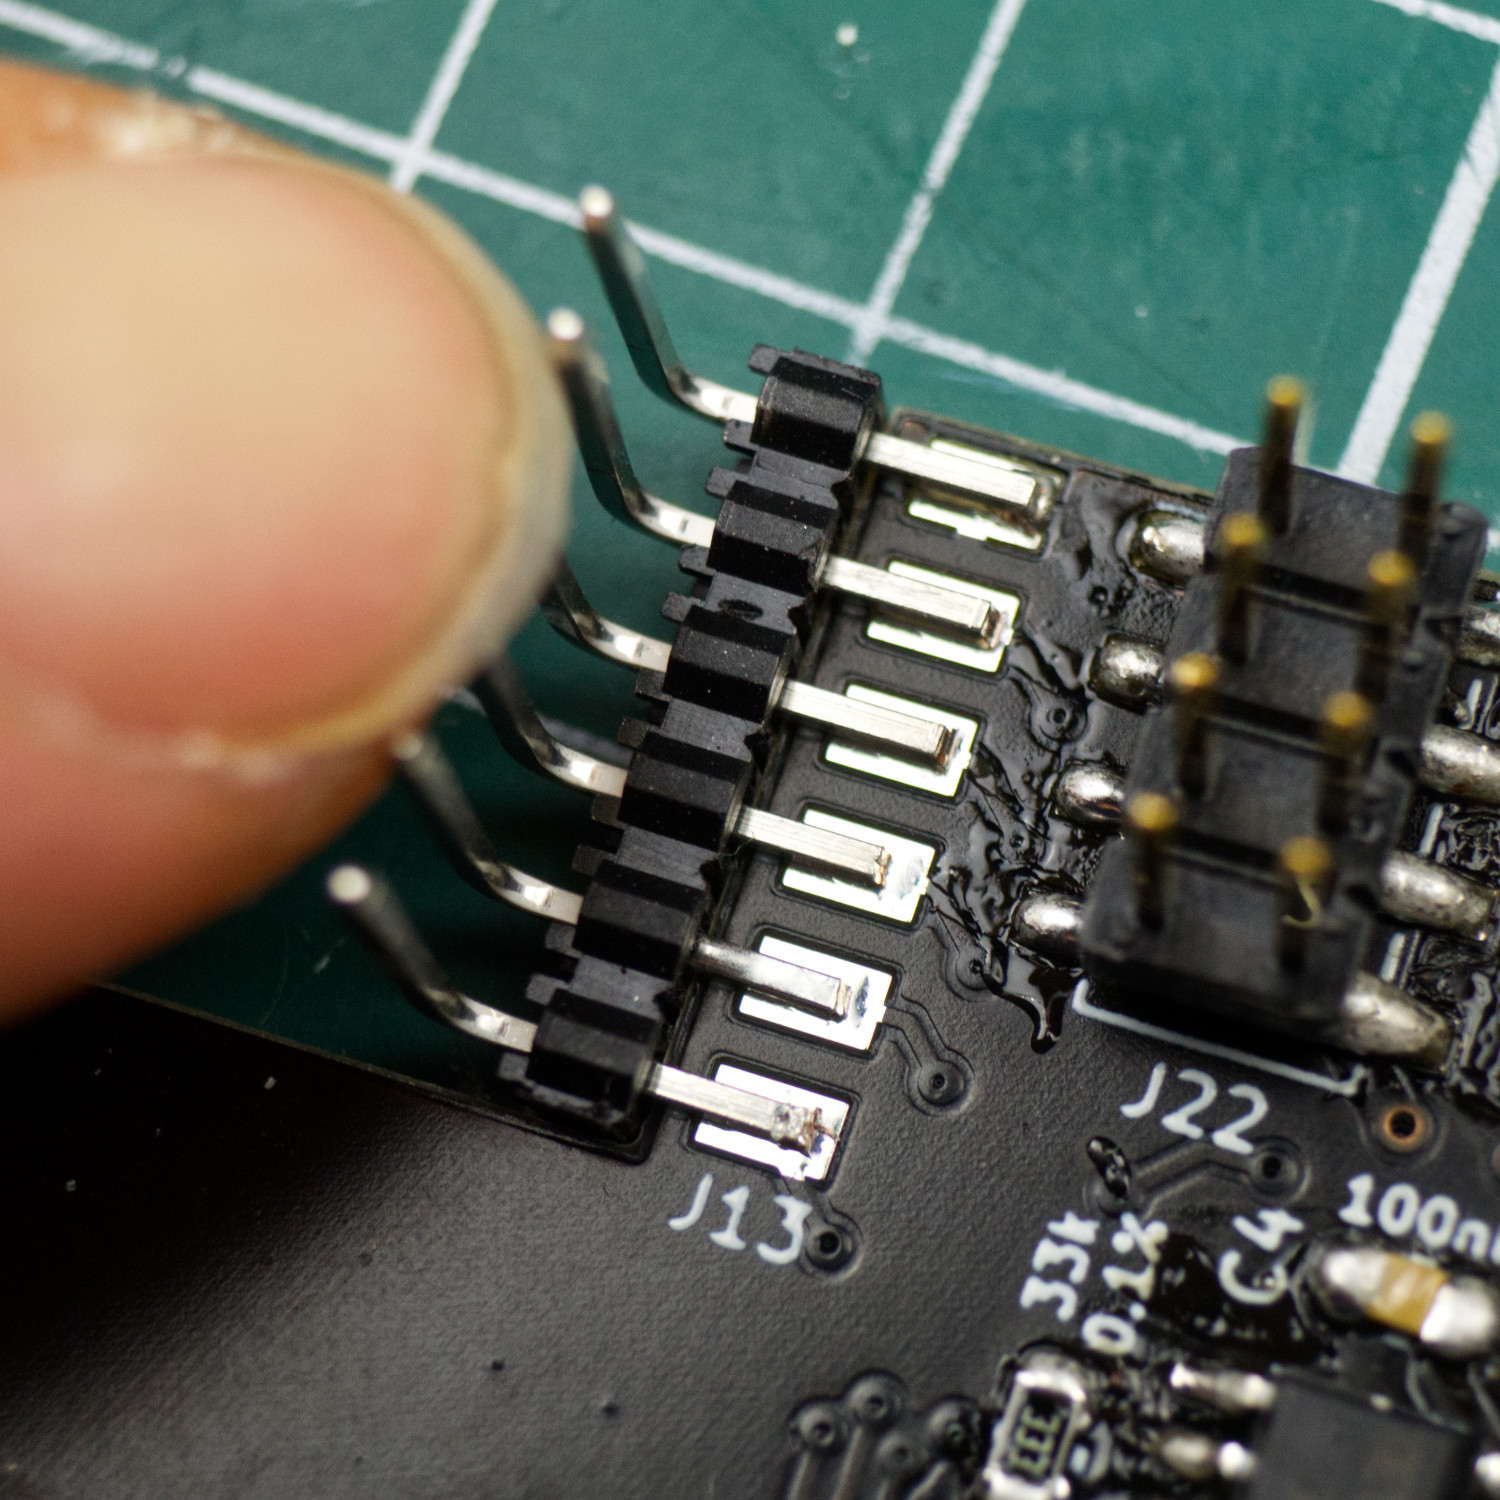
\includegraphics[width=46mm]{images/section_2-2_aligning.jpg}
\end{figure}

Then, for each header, tin one of the pads, reheat it and carefully push the header into the 
corner of the PCB. Make sure they are not crooked and sit flat on the PCB without any vertical
offset.

As before, these have to be aligned reasonably well, although it is a little less critical,
because alignment is generally easier, and they can also be bent into place later on.

\begin{figure}[H]
    \centering
    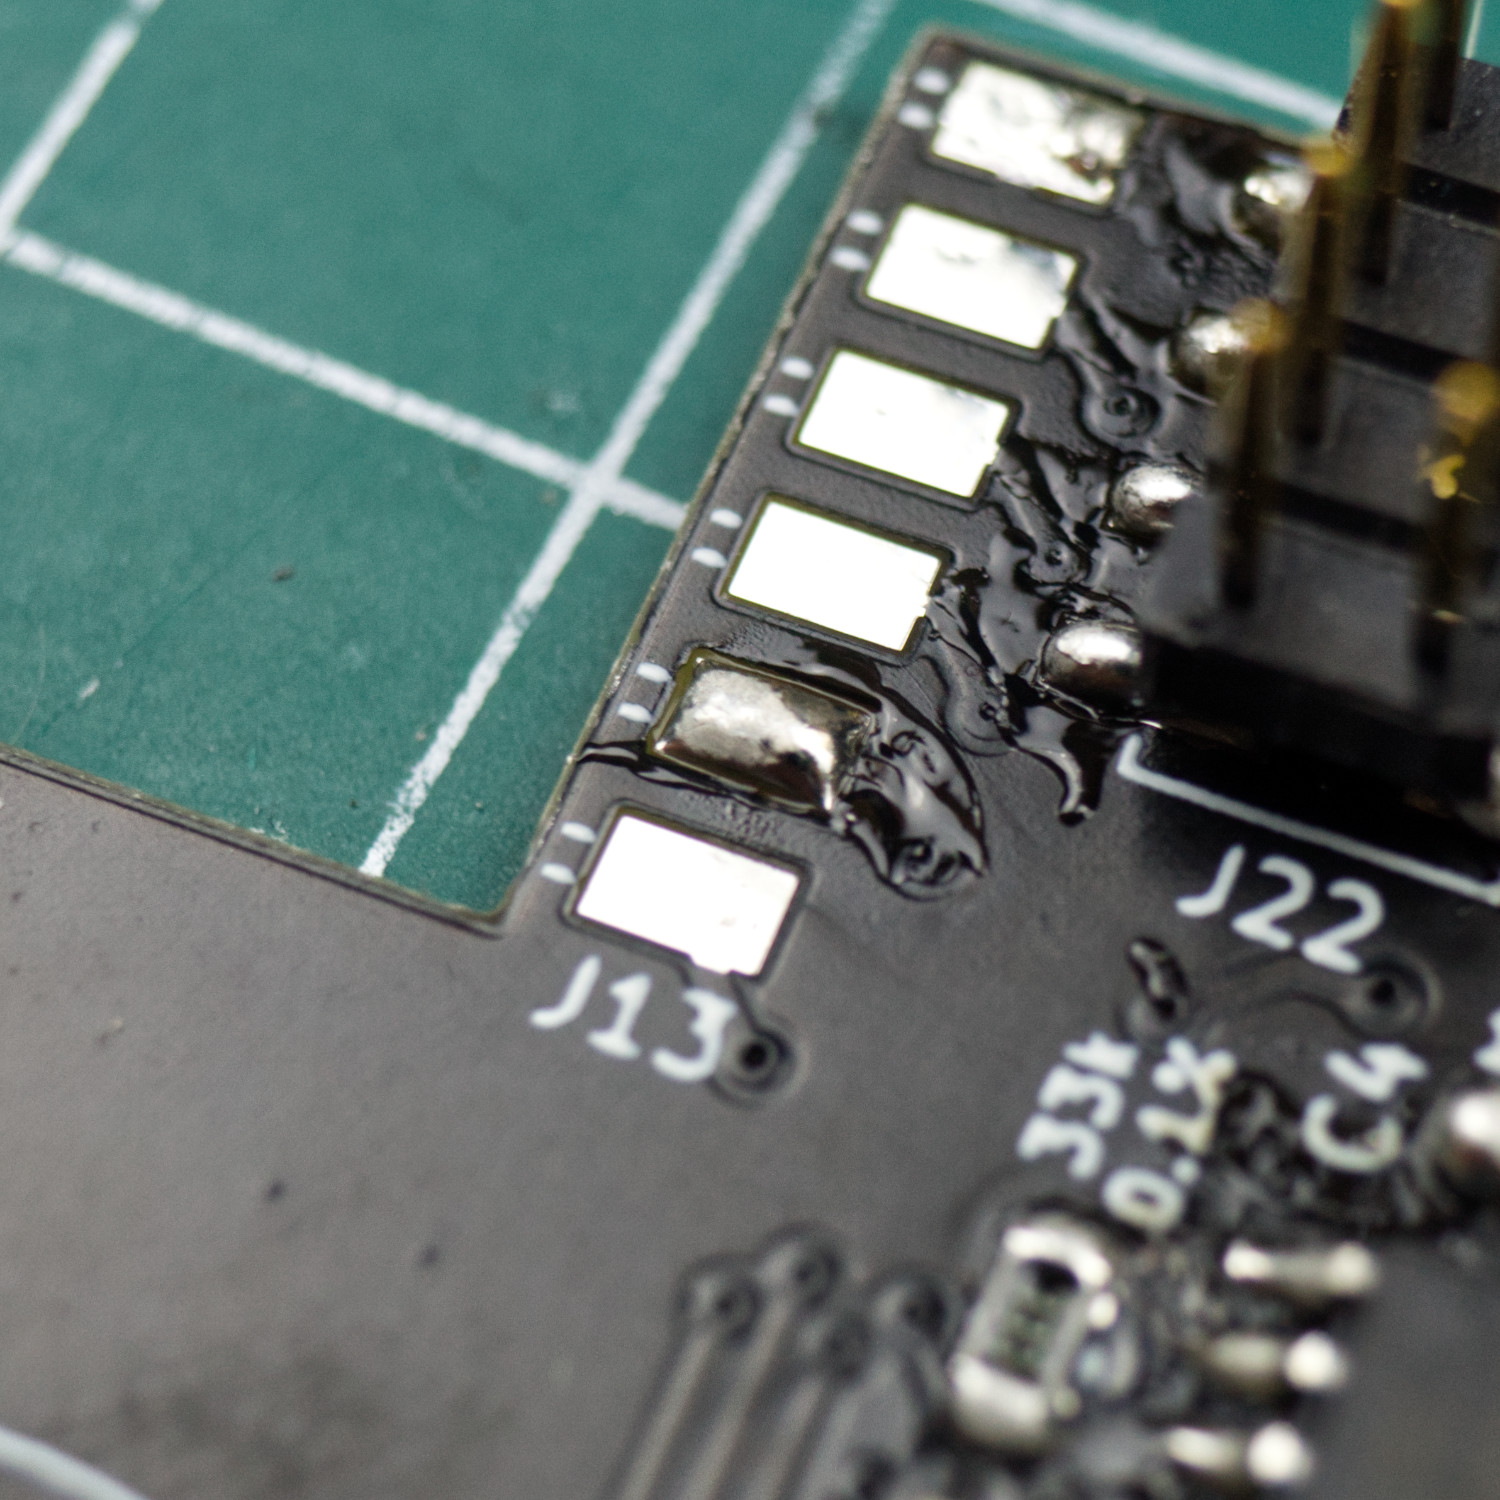
\includegraphics[width=46mm]{images/section_2-2_pad_soldered.jpg}
    \hspace{2mm}
    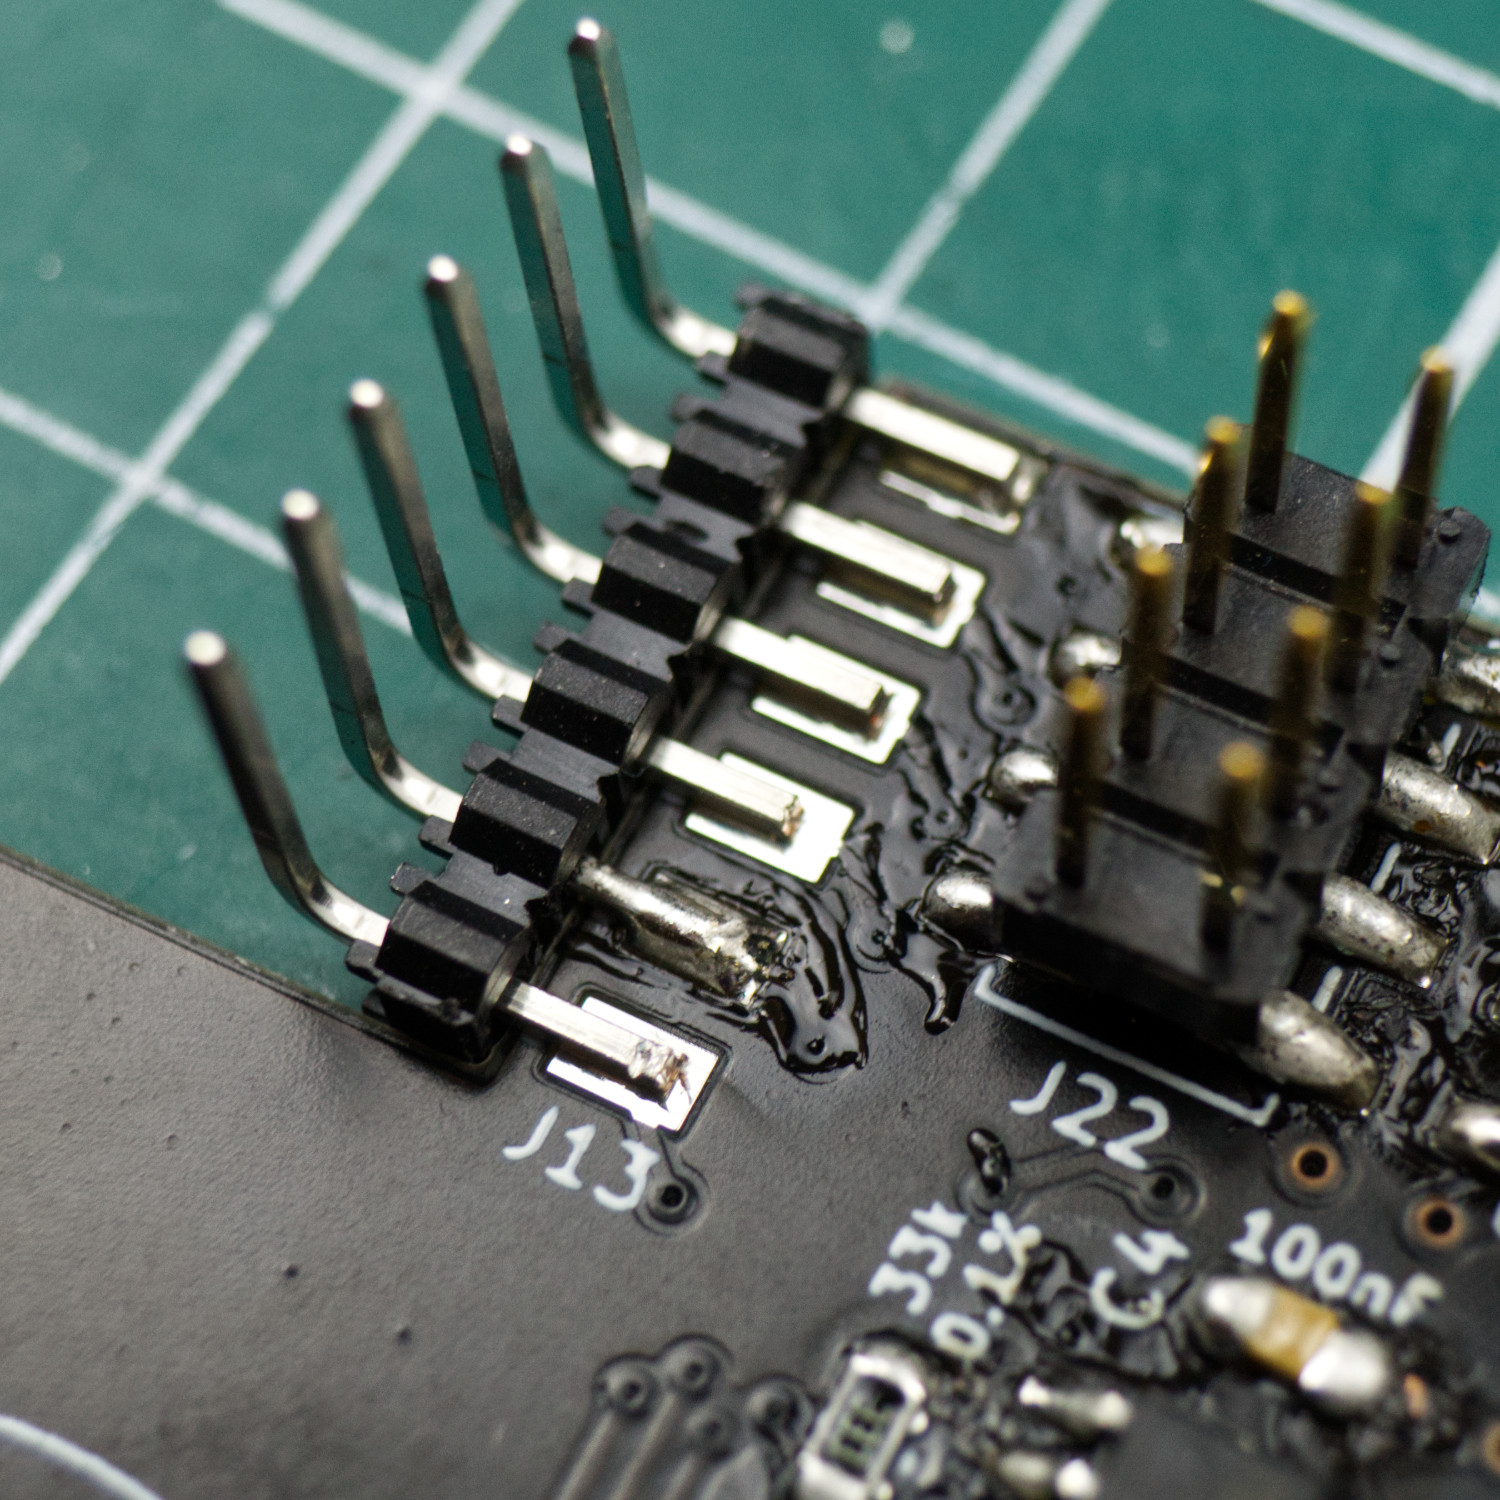
\includegraphics[width=46mm]{images/section_2-2_soldered.jpg}
    \hspace{2mm}
    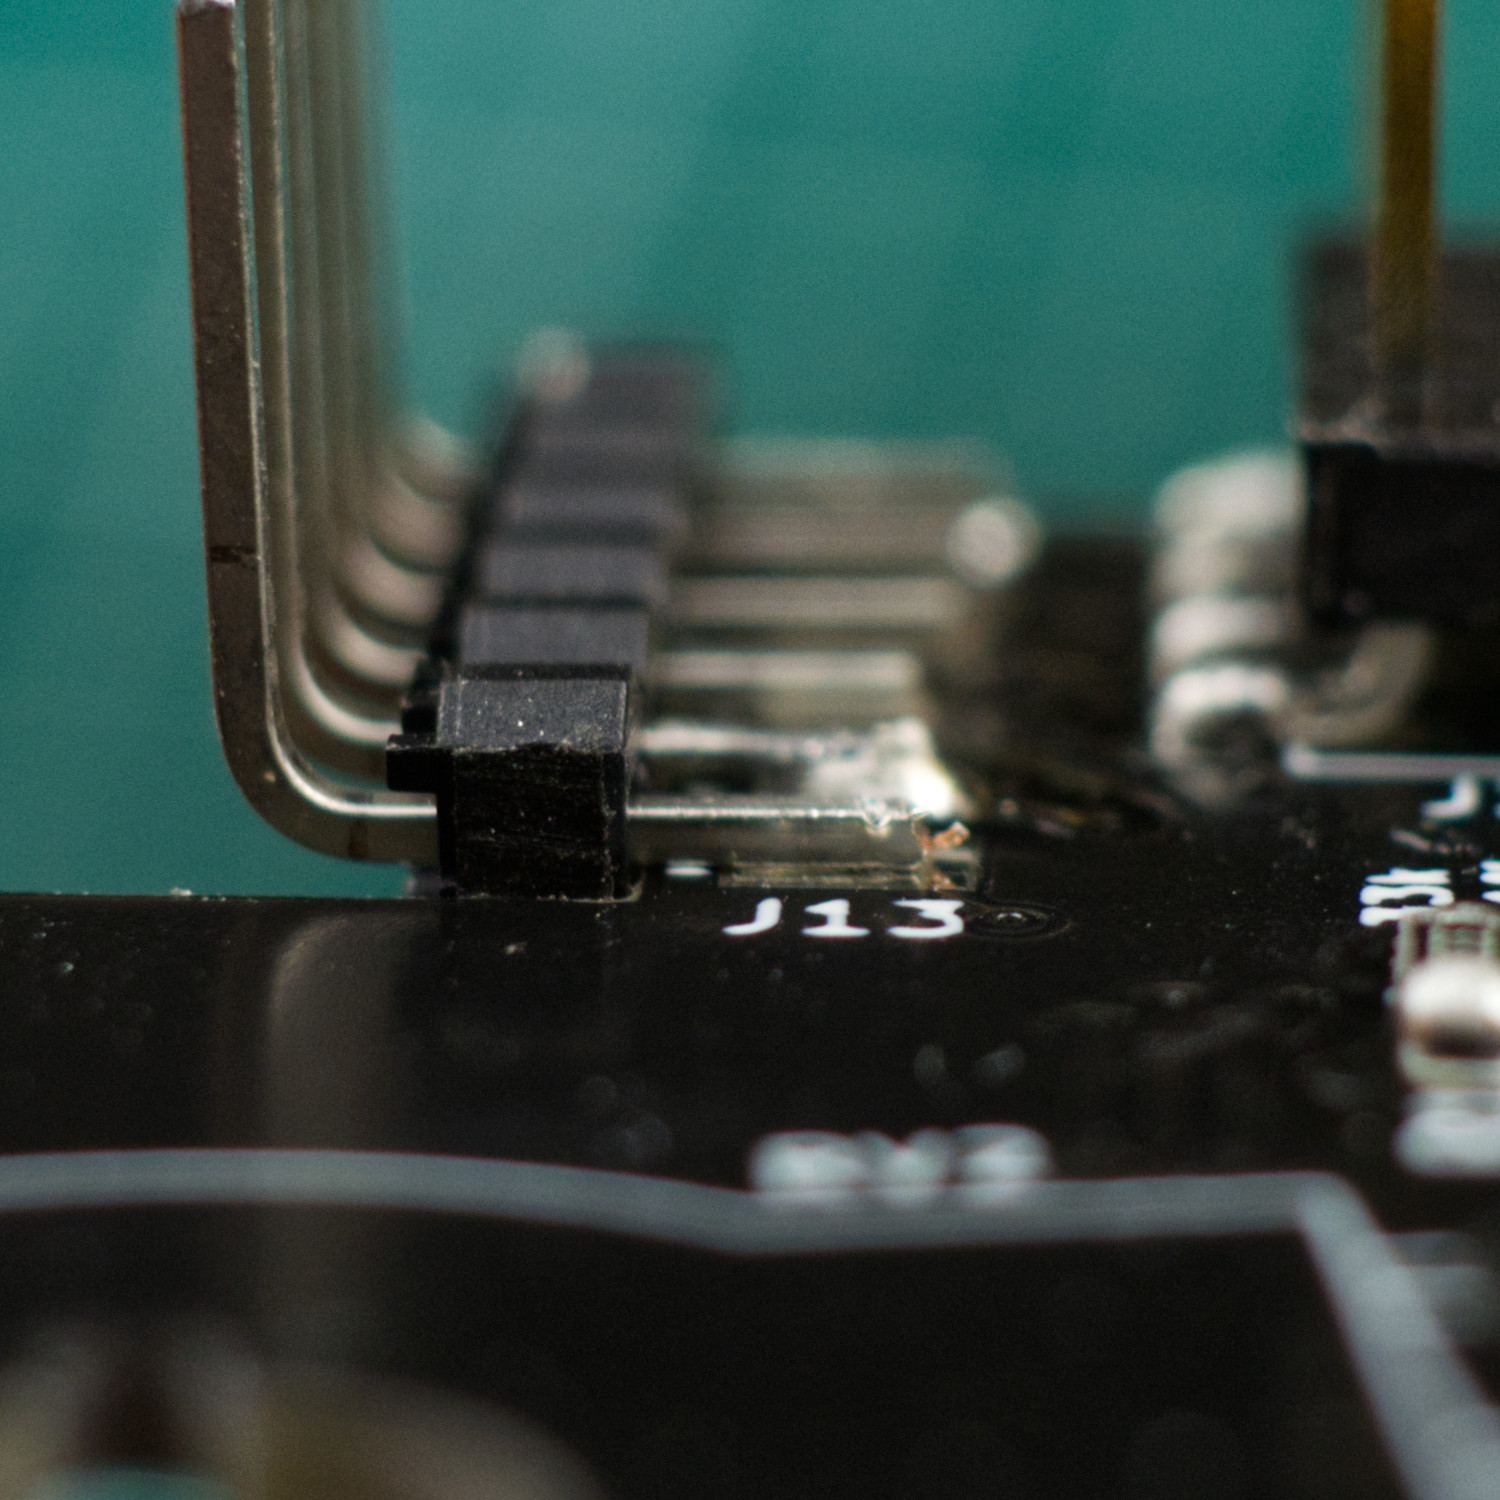
\includegraphics[width=46mm]{images/section_2-2_flat.jpg}
\end{figure}

Finally, solder all the remaining pins.

\pagebreak
\section{Front Panel Components}

\begin{figure}[H]
    \centering
    \begin{tikzpicture}
        \node[anchor=south west,inner sep=0] (image) at (0,0) {
            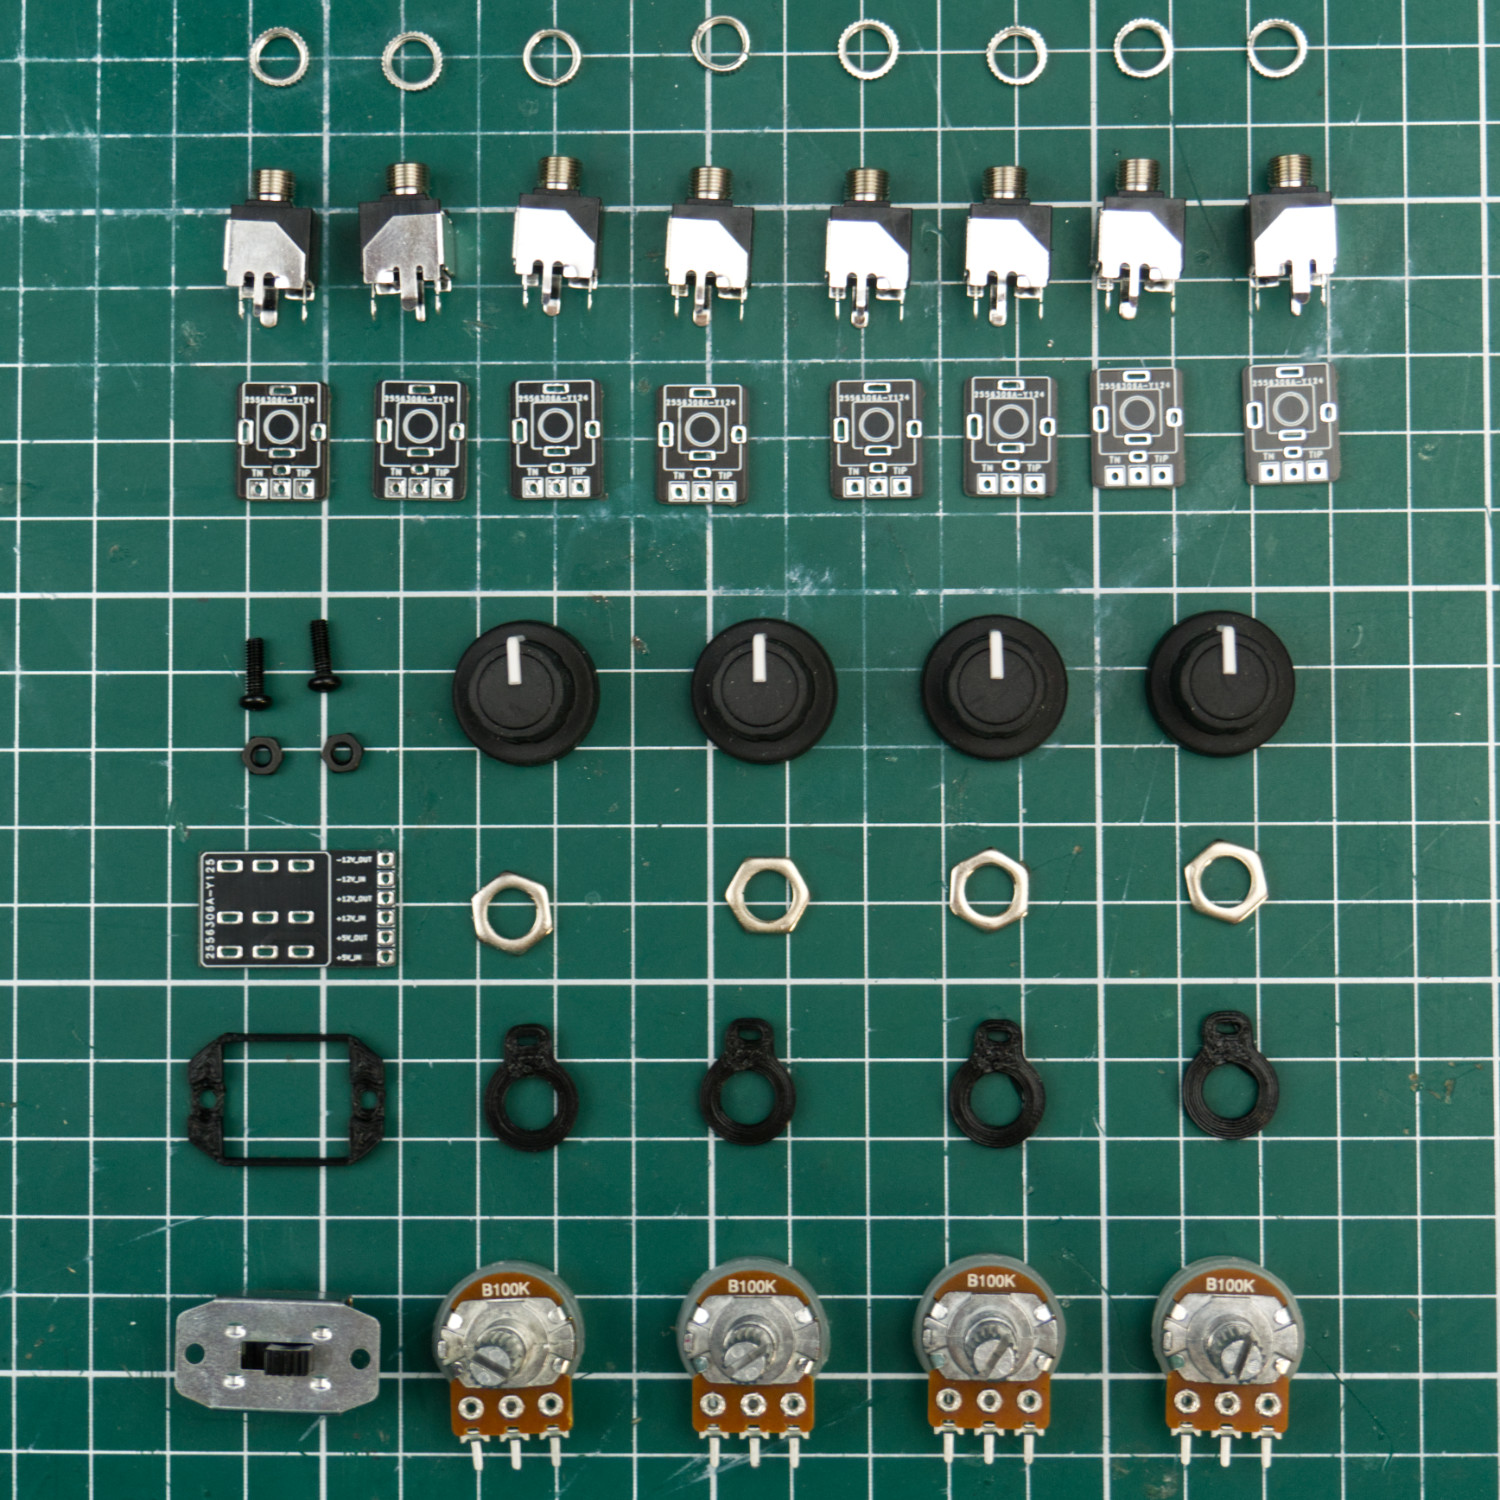
\includegraphics[width=7cm]{images/front_panel_components_topdown.jpg}
        };
        \begin{scope}[x={(image.south east)},y={(image.north west)}]
            \drawrect{0.13, 0.92}{0.91, 0.995} \drawtext{0.52, 0.96}{18}
            \drawrect{0.13, 0.77}{0.91, 0.91} \drawtext{0.52, 0.84}{19}
            \drawrect{0.13, 0.64}{0.91, 0.76} \drawtext{0.52, 0.70}{20}

            \drawrect{0.13, 0.47}{0.26, 0.61} \drawtext{0.19, 0.54}{21}
            \drawrect{0.28, 0.47}{0.88, 0.61} \drawtext{0.59, 0.54}{22}

            \drawrect{0.12, 0.34}{0.28, 0.46} \drawtext{0.20, 0.40}{23}
            \drawrect{0.29, 0.34}{0.88, 0.46} \drawtext{0.59, 0.40}{24}

            \drawrect{0.12, 0.21}{0.27, 0.33} \drawtext{0.19, 0.27}{25}
            \drawrect{0.29, 0.21}{0.88, 0.33} \drawtext{0.59, 0.27}{26}

            \drawrect{0.11, 0.01}{0.27, 0.19} \drawtext{0.19, 0.15}{27}
            \drawrect{0.28, 0.01}{0.88, 0.19} \drawtext{0.58, 0.15}{28}
        \end{scope}
    \end{tikzpicture}
    \hspace{2mm}
    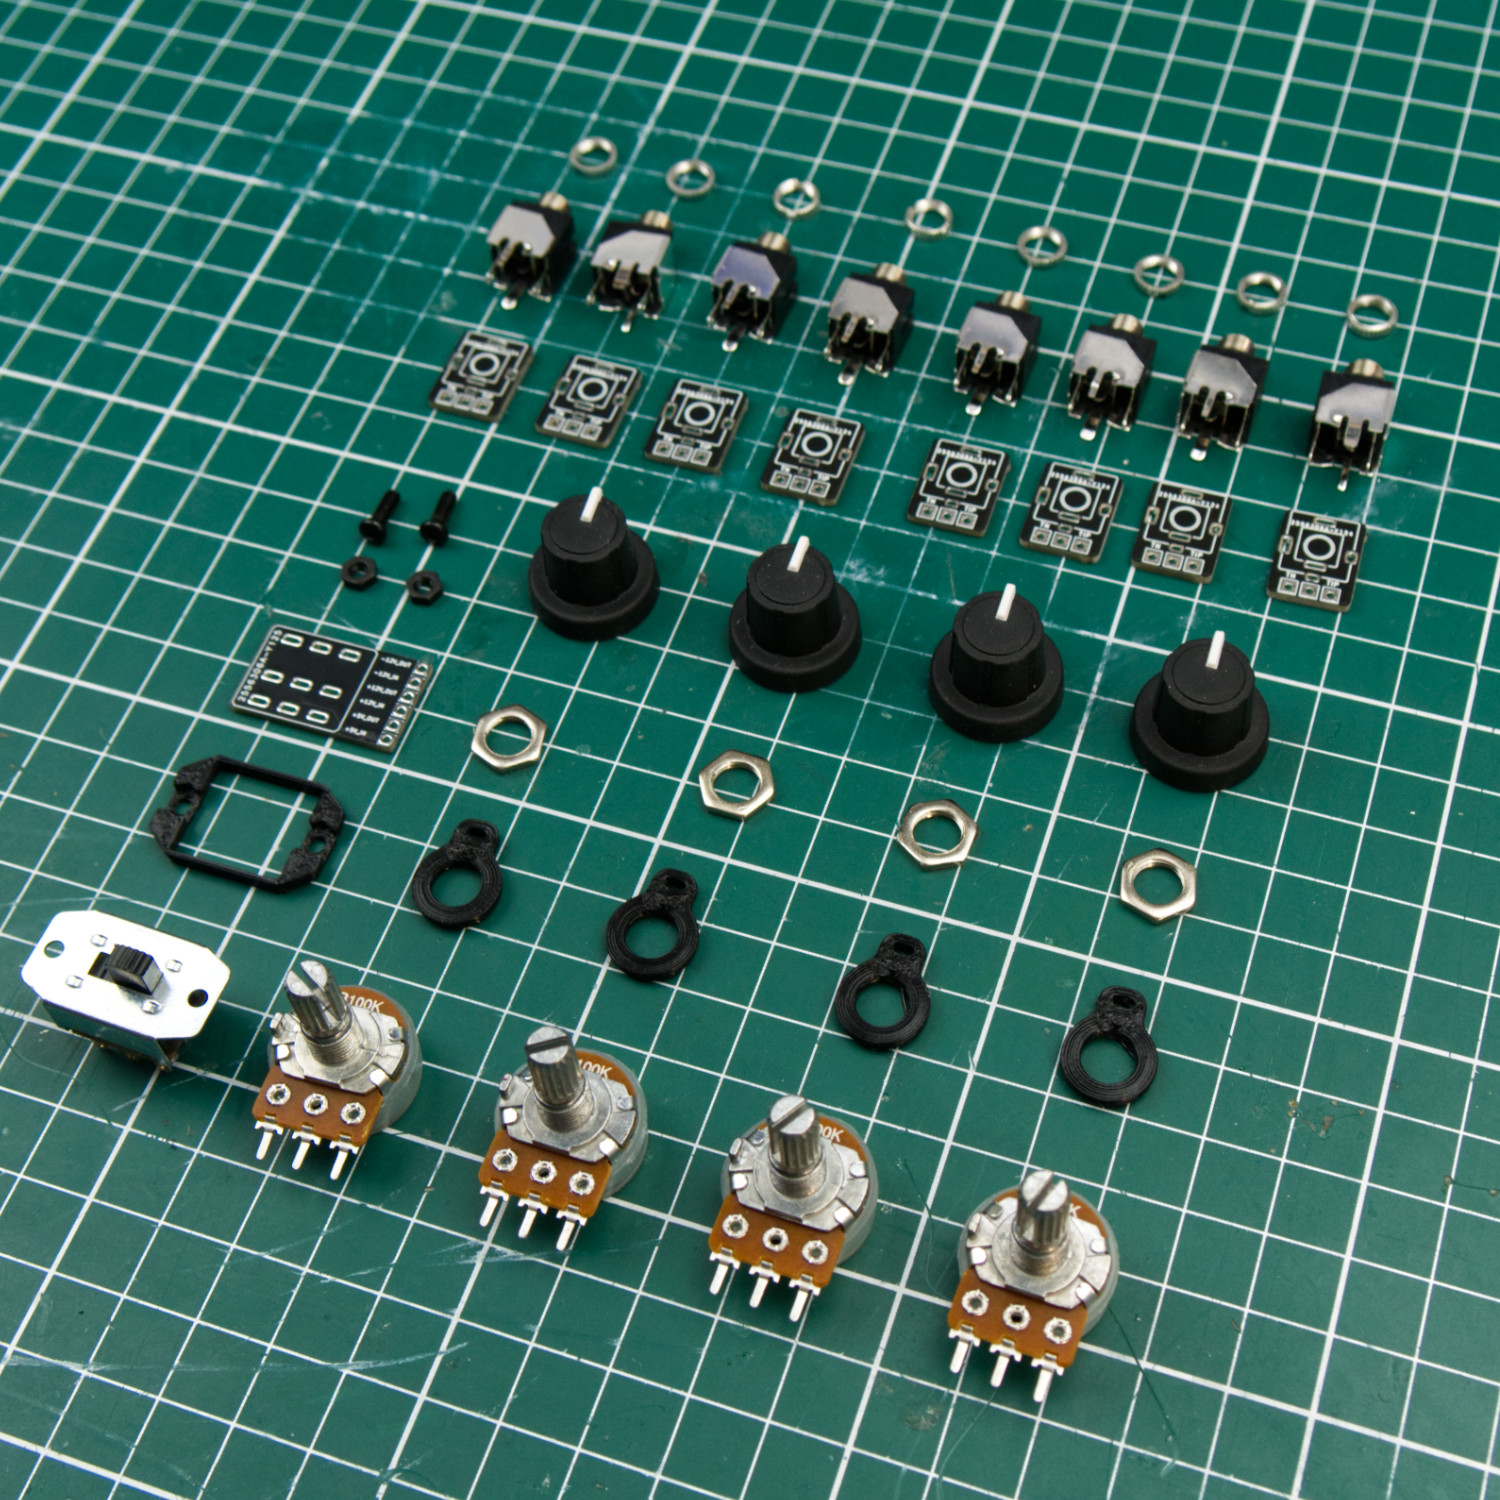
\includegraphics[width=7cm]{images/front_panel_components_side.jpg}
\end{figure}

\begin{center}
    \small
    \setlength\extrarowheight{4pt}
    \begin{tabularx}{\textwidth}{|c|c|X|l|}
        \hline \rowcolor{lightgray} ID & Qty & Description & PCB Identifier / Ref\\
        \hline 20 & 8 & Knurled Nut & -\\
        \hline 21 & 8 & WQP518MA-BM Audio Jack & J2, J3, J4, J5, J6. J7, J8, J9\\
        \hline 22 & 8 & Audio Jack PCB & -\\
        \hline 23 & 2 & M2 Screw, Nut & -\\
        \hline 24 & 1 & Power Switch & SW1\\
        \hline 25 & 1 & Power Switch Bracket & -\\
        \hline 26 & 1 & Power Switch PCB & -\\
        \hline 27 & 4 & Potentiometer Knob & -\\
        \hline 28 & 4 & Potentiometer Nut & -\\
        \hline 29 & 4 & Potentiometer Spacer & -\\
        \hline 30 & 4 & 100k Potentiometer (linear) & RV1, RV2, RV3, RV4\\
        \hline 31 & 4 & Potentiometer Dust Covers & -\\
        \hline 32 & 1 & 0.8mm Tinned Copper Wire (75cm) & -\\
        \hline
    \end{tabularx}
\end{center}

\pagebreak
\subsection{Power Switch}

\begin{center}
    \small
    \setlength\extrarowheight{8pt}
    \begin{tabularx}{\textwidth}{|c|c|c|X|l|}
        \hline\rowcolor{lightgray} & ID & Qty & Description & PCB Identifier\\
        \hline\checkbox{ha} & 23 & 2 & M2 Screw, Nut & -\\
        \hline\checkbox{hb} & 25 & 1 & Power Switch Bracket & -\\
        \hline\checkbox{hc} & 24 & 1 & Power Switch & SW1\\
        \hline\checkbox{hd} & 26 & 1 & Power Switch PCB & -\\
        \hline
    \end{tabularx}
\end{center}

Insert the two M2 nuts into the 3D printed plastic bracket and slip it onto the switch (with
the M2 nuts facing away from the switch).

Next, hold the switch against the main PCB and screw it in place using the two M2 screws and a
1.5mm hex key. \textbf{Be careful to put it on the right way. The two rows of pins on the back
of the switch that are closer to each other should be facing towards the power connector.}

Add the Power Switch PCB to the switch (blank side up), push it down and solder down all the
pins.

\begin{figure}[H]
    \centering
    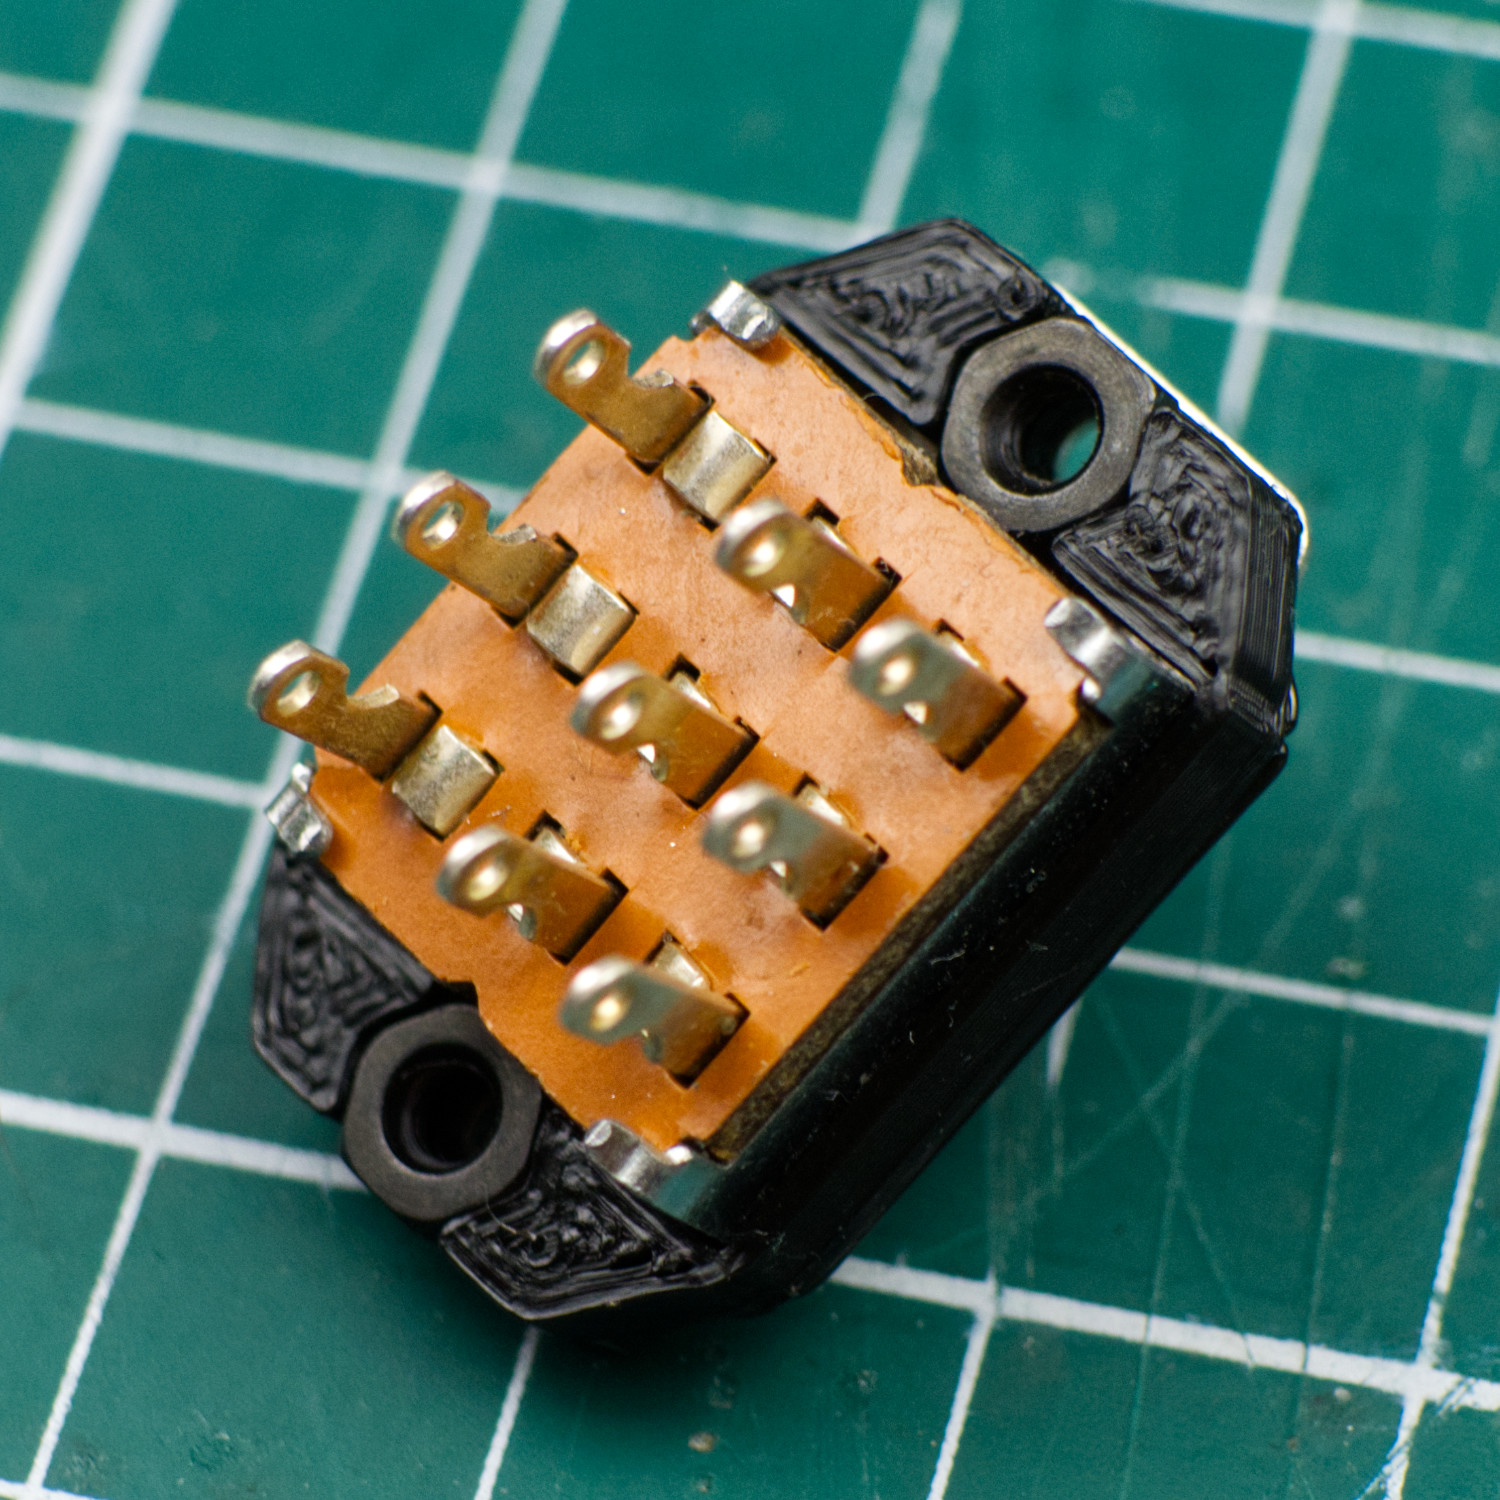
\includegraphics[width=46mm]{images/section_3-1_bracket.jpg}
    \hspace{2mm}
    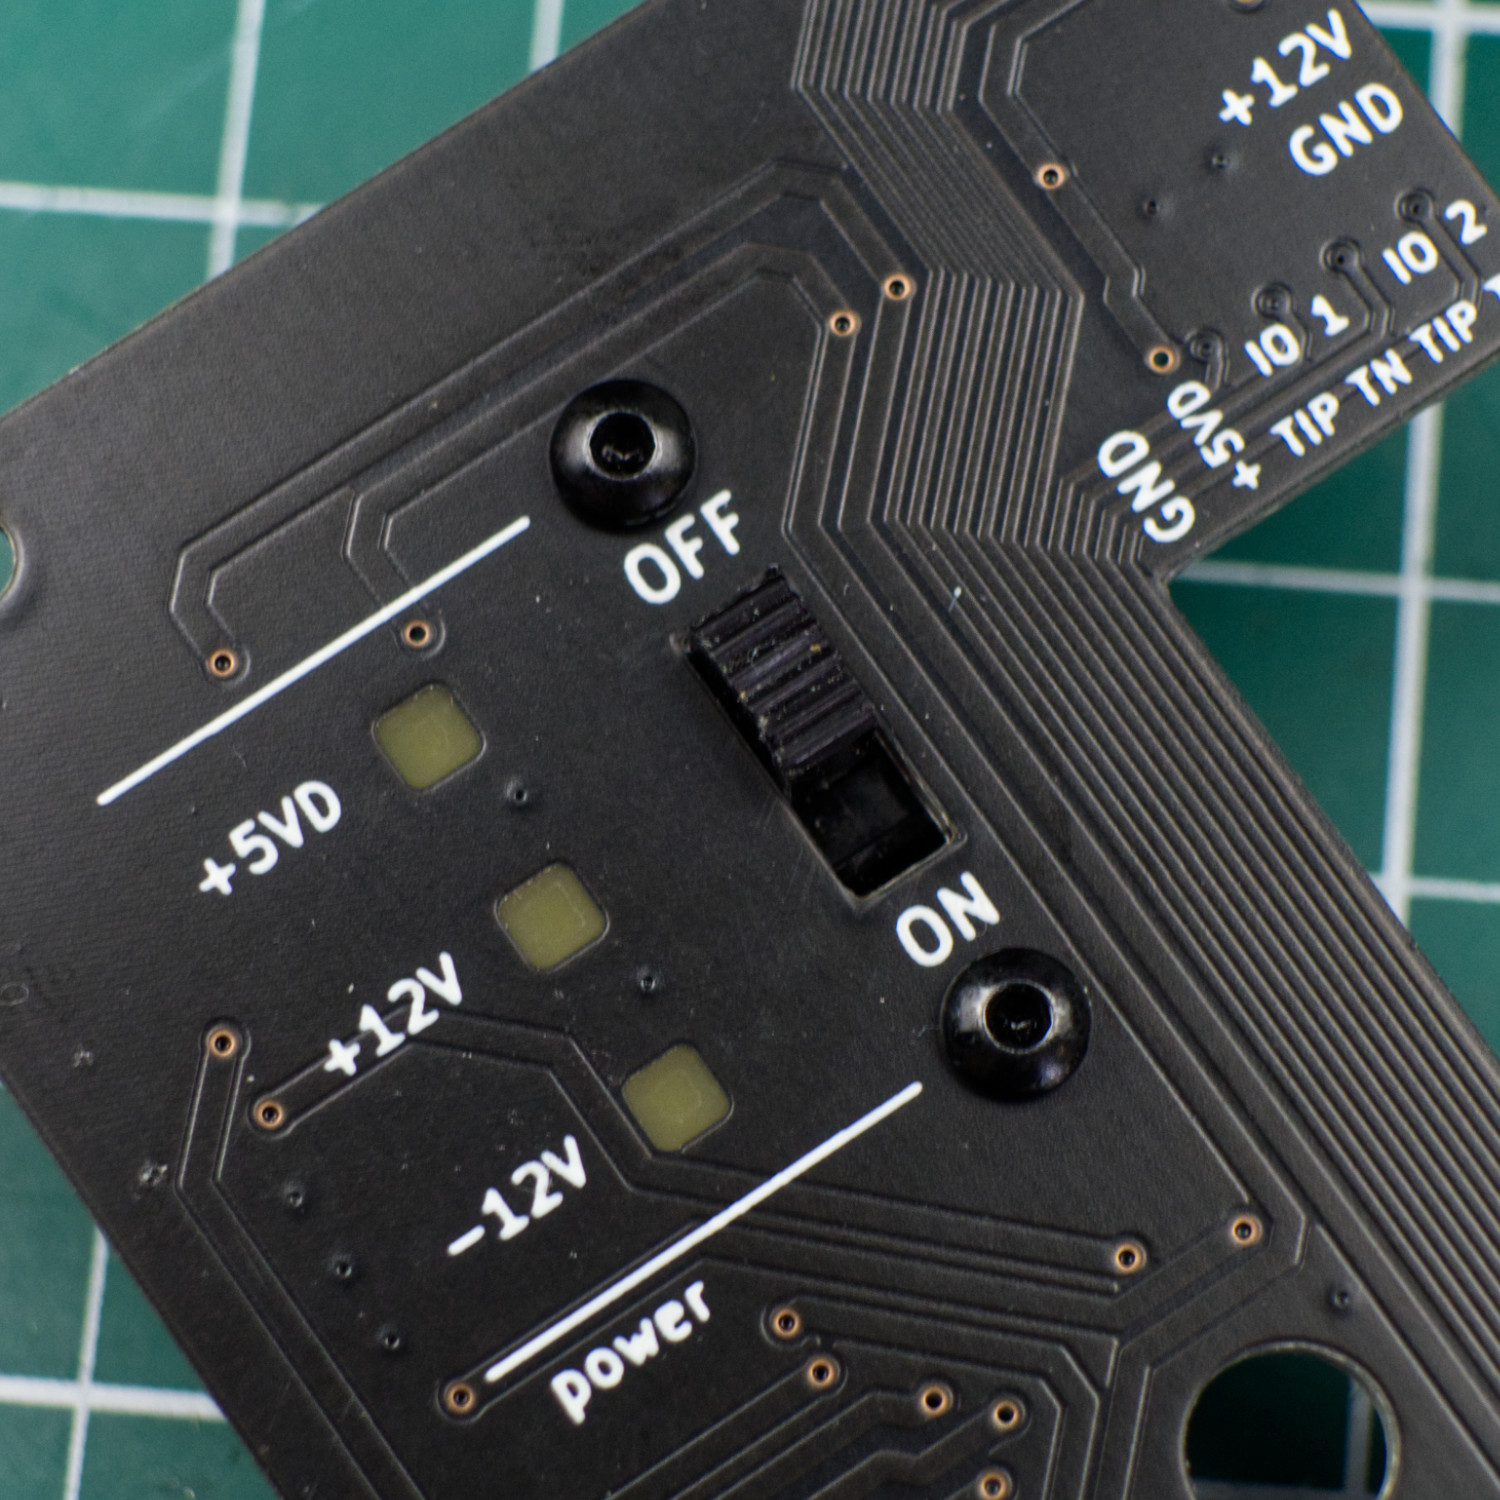
\includegraphics[width=46mm]{images/section_3-1_screwed.jpg}
    \hspace{2mm}
    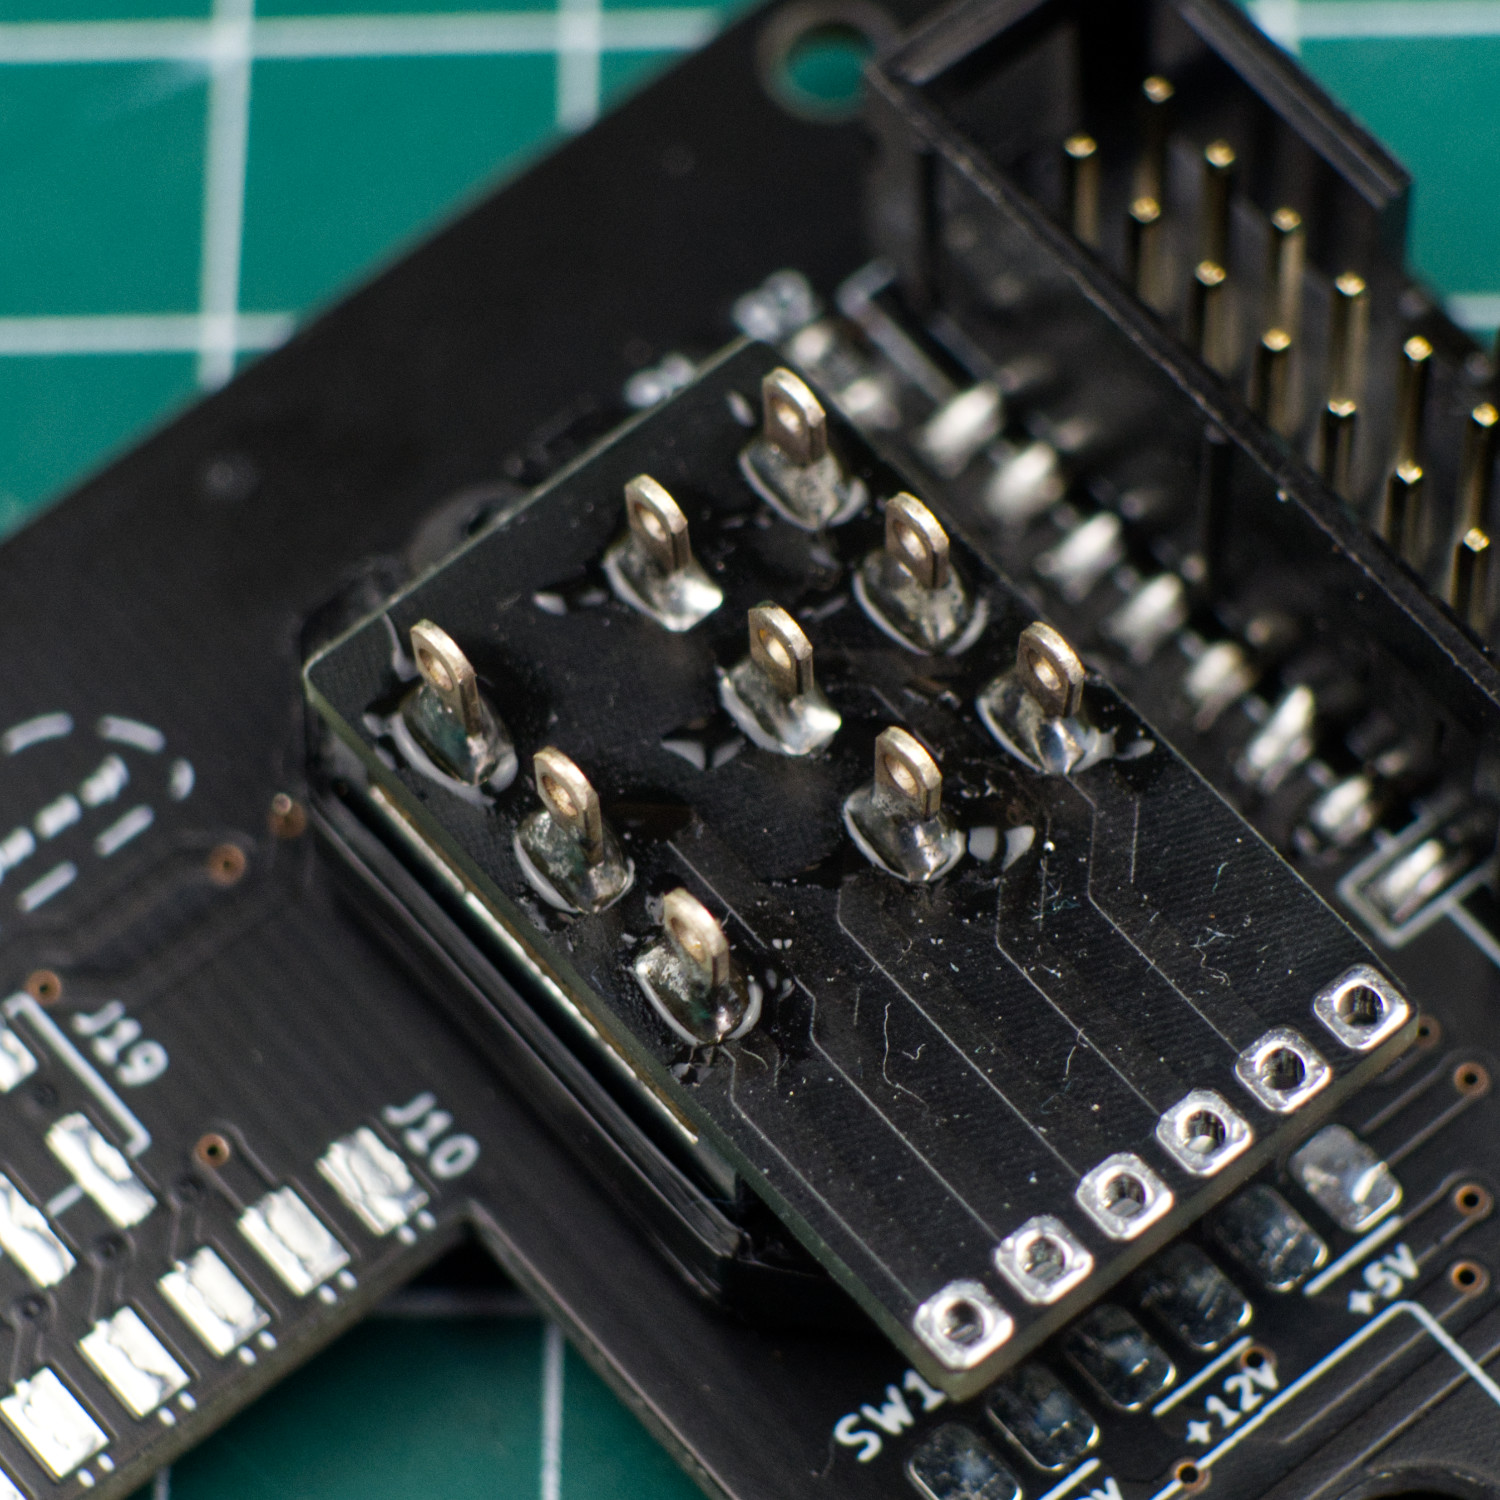
\includegraphics[width=46mm]{images/section_3-1_soldered.jpg}
\end{figure}

Snip off six \textbf{\textasciitilde12mm} pieces of the solid core wire and put each of them through
one of the through-holes on the switch PCB. Fix them in place by soldering them to the pad
on the main PCB first, then make sure they are straight and solder the pad on the switch PCB.

Finally, use your multimeter in continuity mode to ensure you did not create any short-circuits.
With the switch being in the OFF position, there should not be continuity between any of the
wires.

\subsection{Testing}

TODO

\subsection{3.5mm Jacks}

\begin{center}
    \small
    \setlength\extrarowheight{8pt}
    \begin{tabularx}{\textwidth}{|c|c|c|X|l|}
        \hline\rowcolor{lightgray} & ID & Qty & Description & PCB Identifier\\
        \hline\checkbox{ia} & 20 & 8 & Knurled Nut & -\\
        \hline\checkbox{ib} & 21 & 8 & WQP518MA-BM Audio Jack & J2, J3, J4, J5, J6. J7, J8, J9\\
        \hline\checkbox{ic} & 22 & 8 & Audio Jack PCB & -\\
        \hline
    \end{tabularx}
\end{center}

\vspace{-5mm}
{
    \color{red}
    \subsubsection*{Important:}
    \vspace{-3mm}
    Do each of the following steps for each pair/row of audio jacks, \textbf{one pair/row at a
    time, from top to bottom}. Once a row is assembled, it will be \textbf{nearly impossible
    to reach the one above it}. Make sure your soldering is solid, and there are no shorts.
    \vspace{5mm}
}

Take two audio jacks and knurled nuts and attach them to the two holes on the first row
(from top to bottom) of the PCB. Align them so that they fit into the box marked on the
back side of the PCB.

Add two audio jack PCBs to the audio jacks and solder all the pins.

\begin{figure}[H]
    \centering
    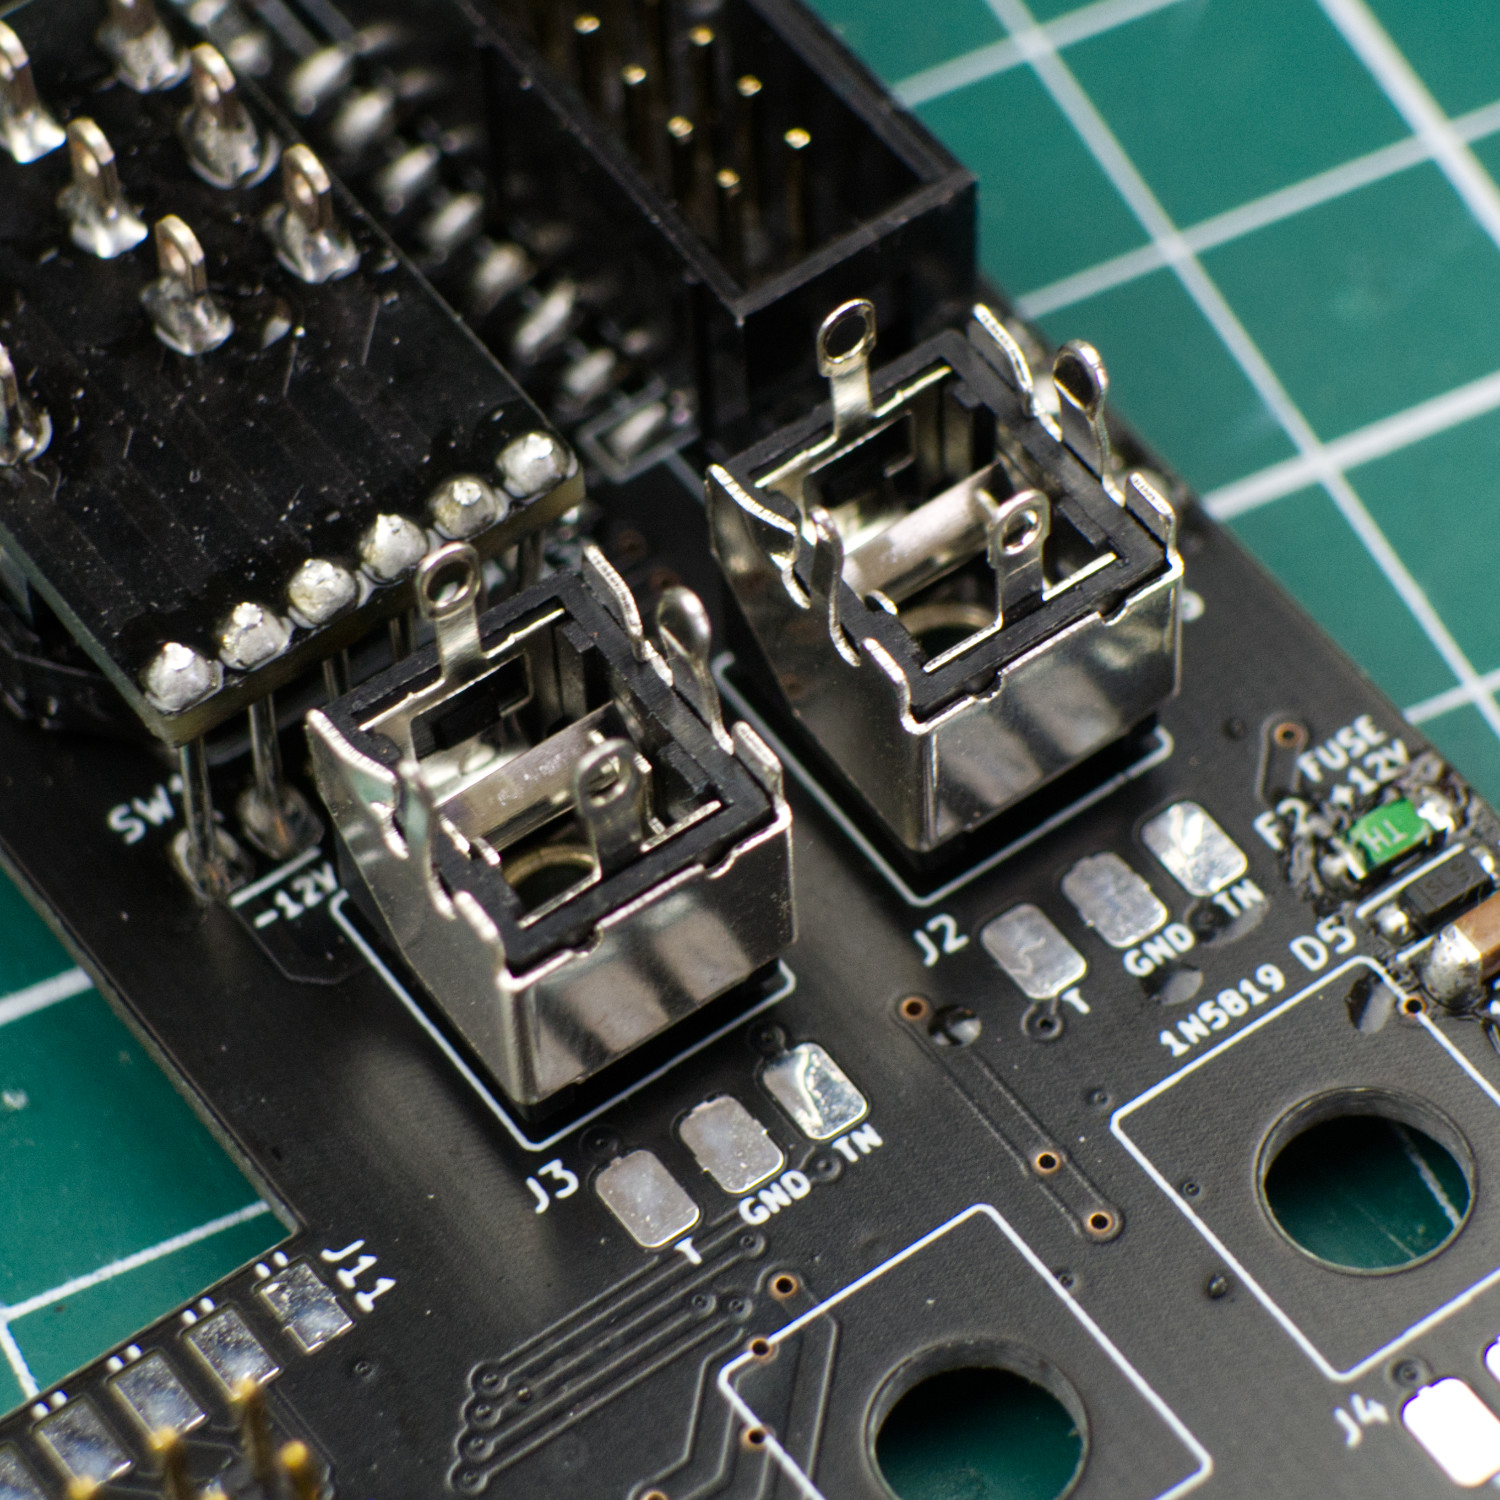
\includegraphics[width=46mm]{images/section_3-3_screwed.jpg}
    \hspace{2mm}
    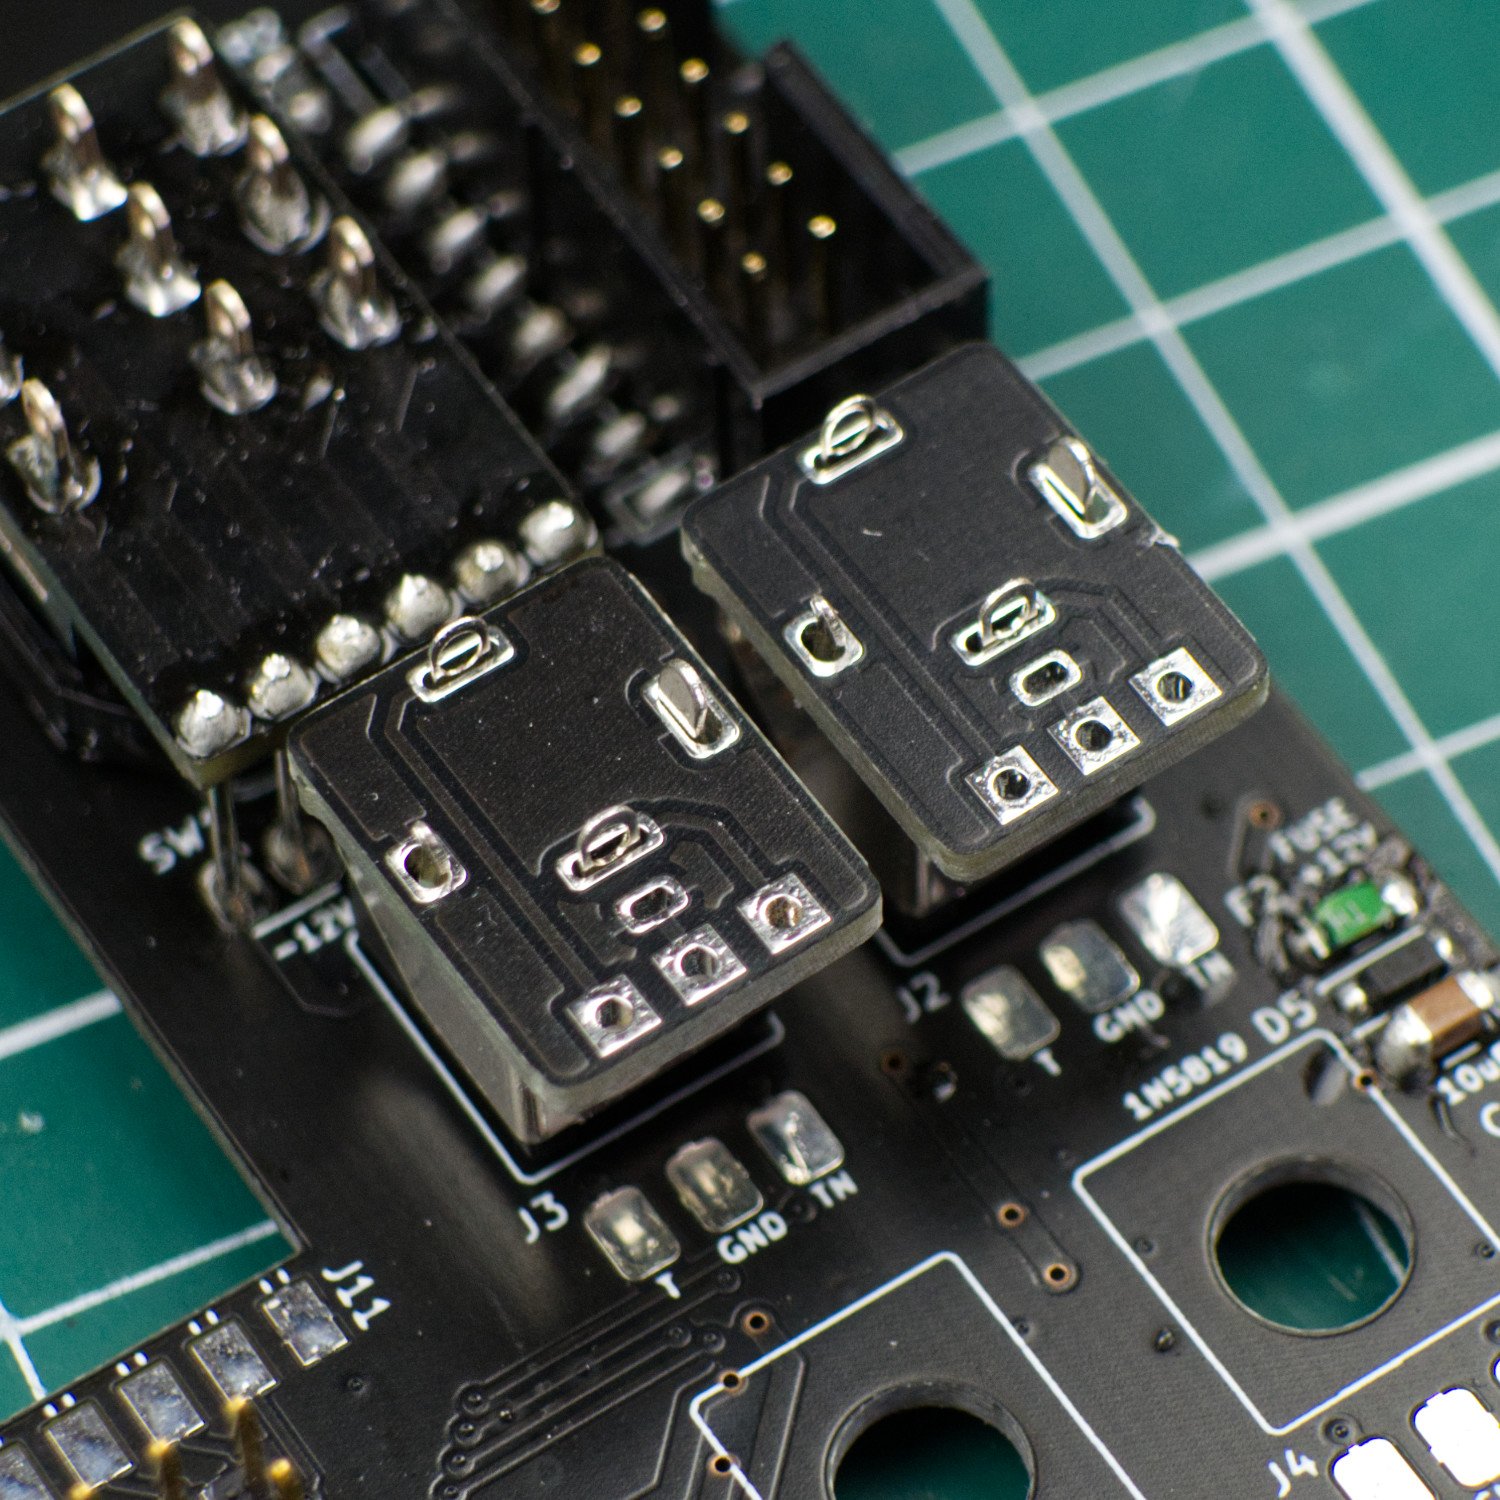
\includegraphics[width=46mm]{images/section_3-3_pcb.jpg}
    \hspace{2mm}
    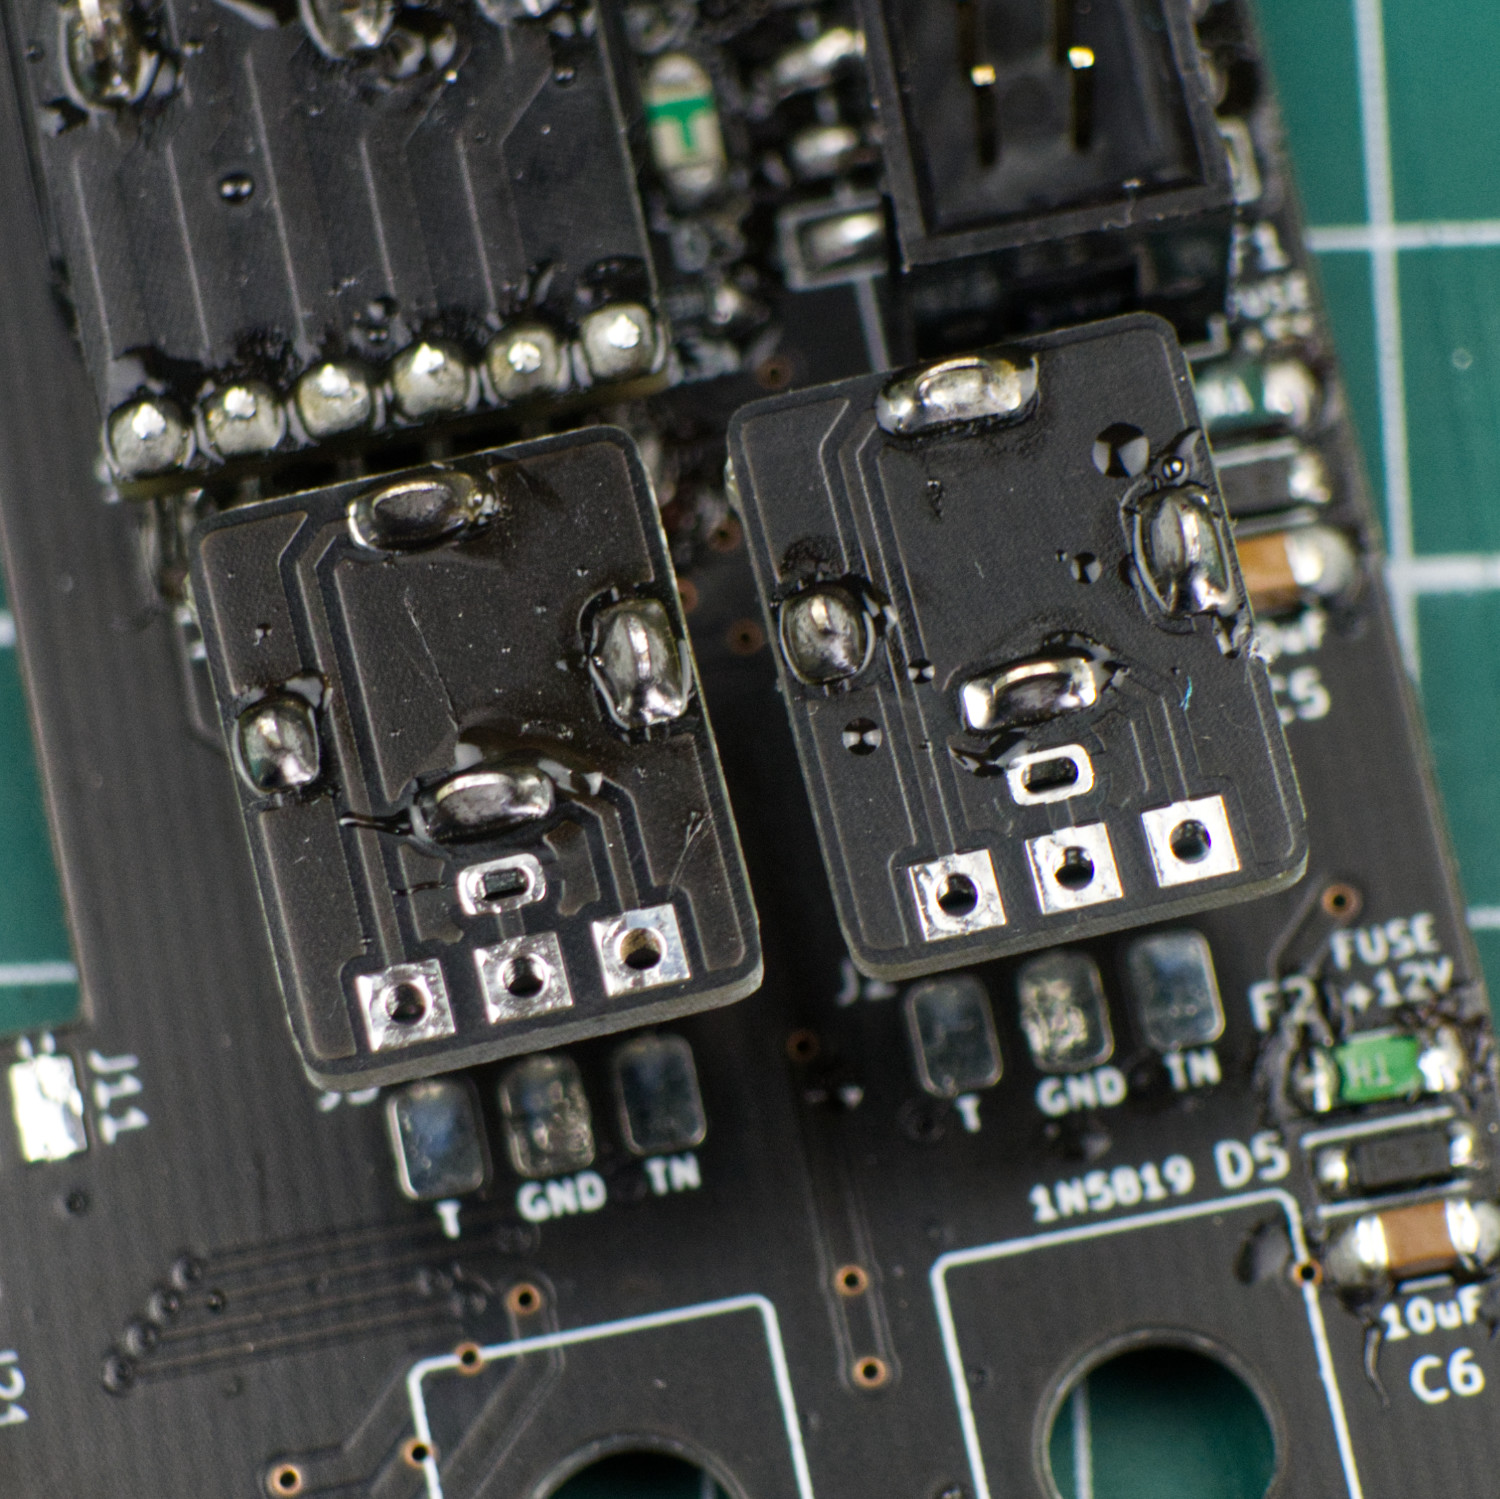
\includegraphics[width=46mm]{images/section_3-3_pcb_soldered.jpg}
\end{figure}

Next, snip off six \textbf{\textasciitilde15mm} pieces of the solid core wire and put each of them
through one of the through-holes on the audio jack PCBs. Fix them in place by soldering them to
the pad on the main PCB first, then make sure they are straight and solder the pad on the audio
jack PCB.

\begin{figure}[H]
    \centering
    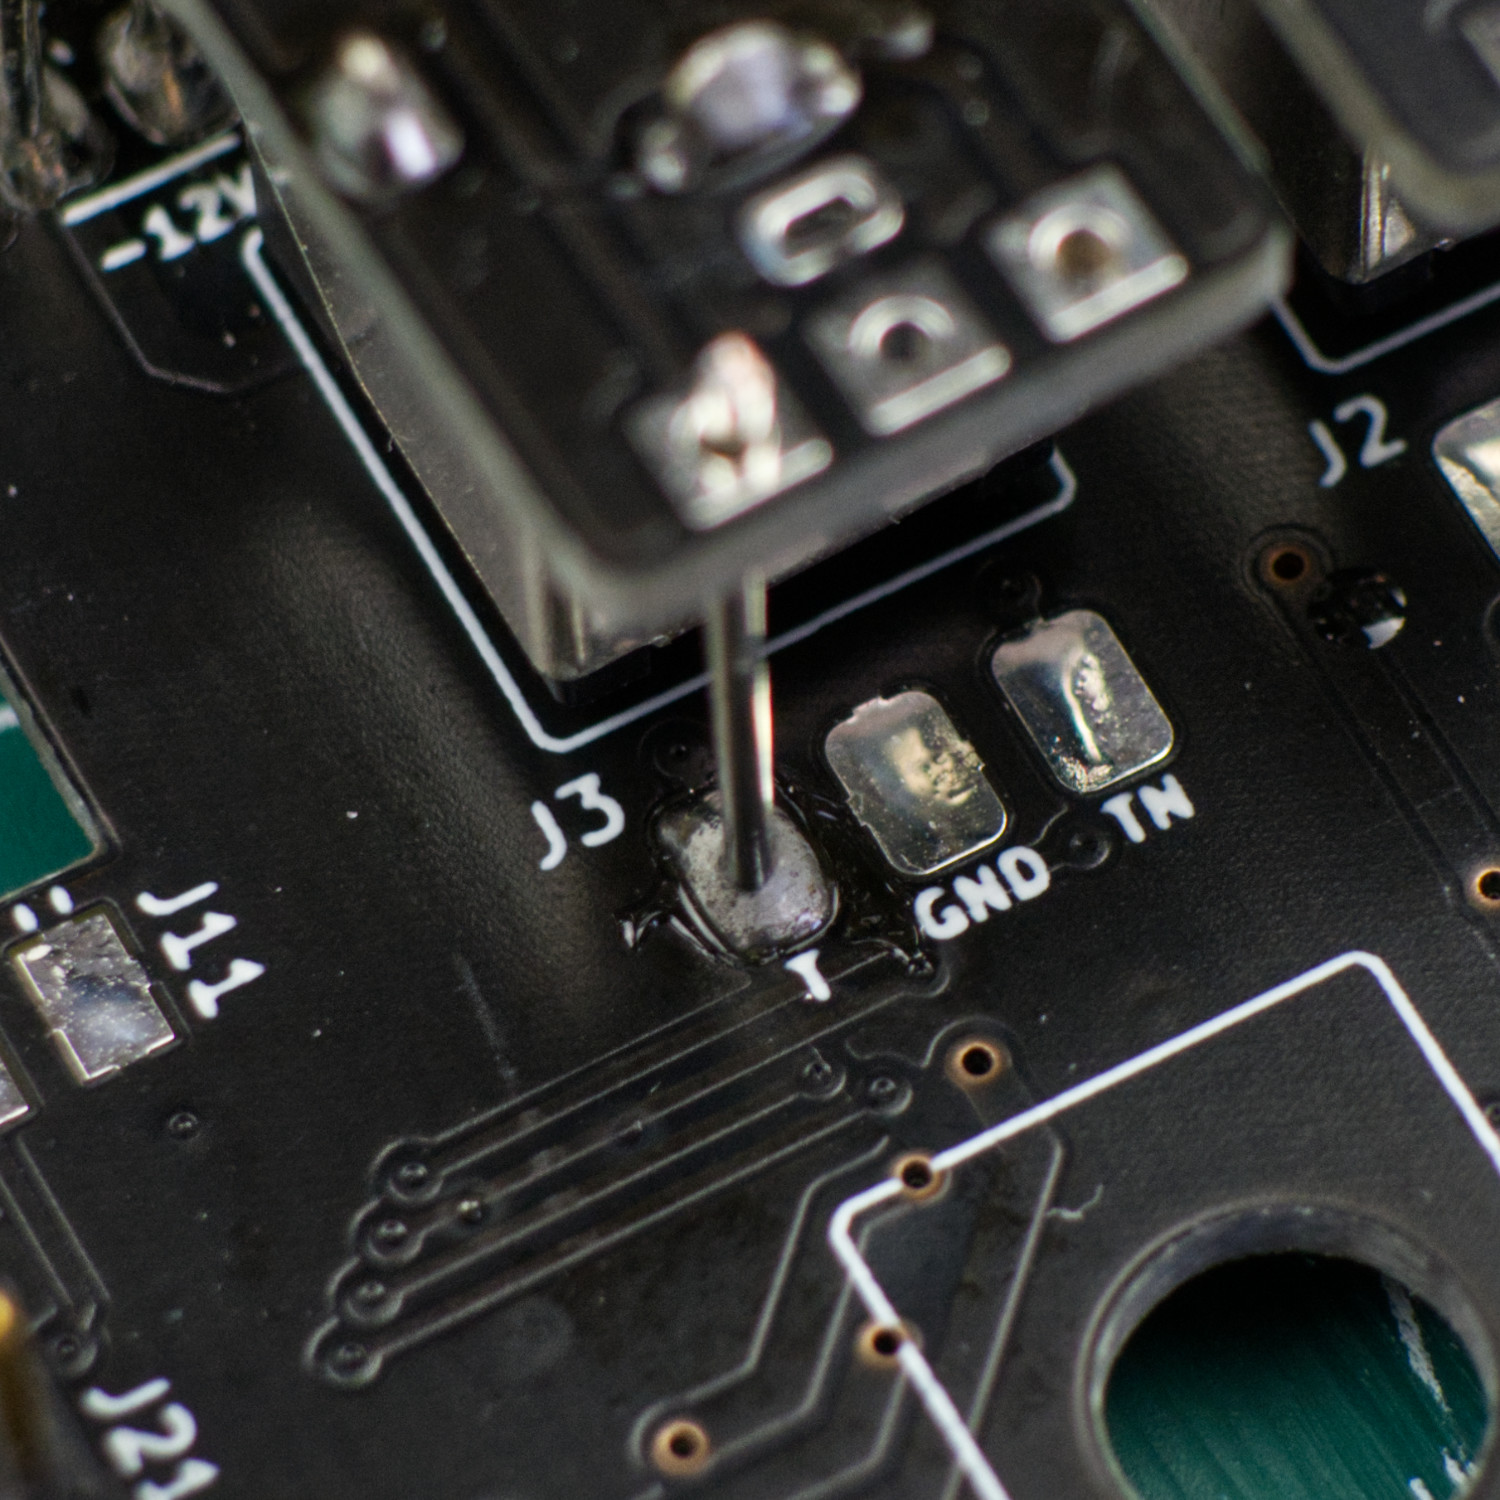
\includegraphics[width=46mm]{images/section_3-3_single_bot.jpg}
    \hspace{2mm}
    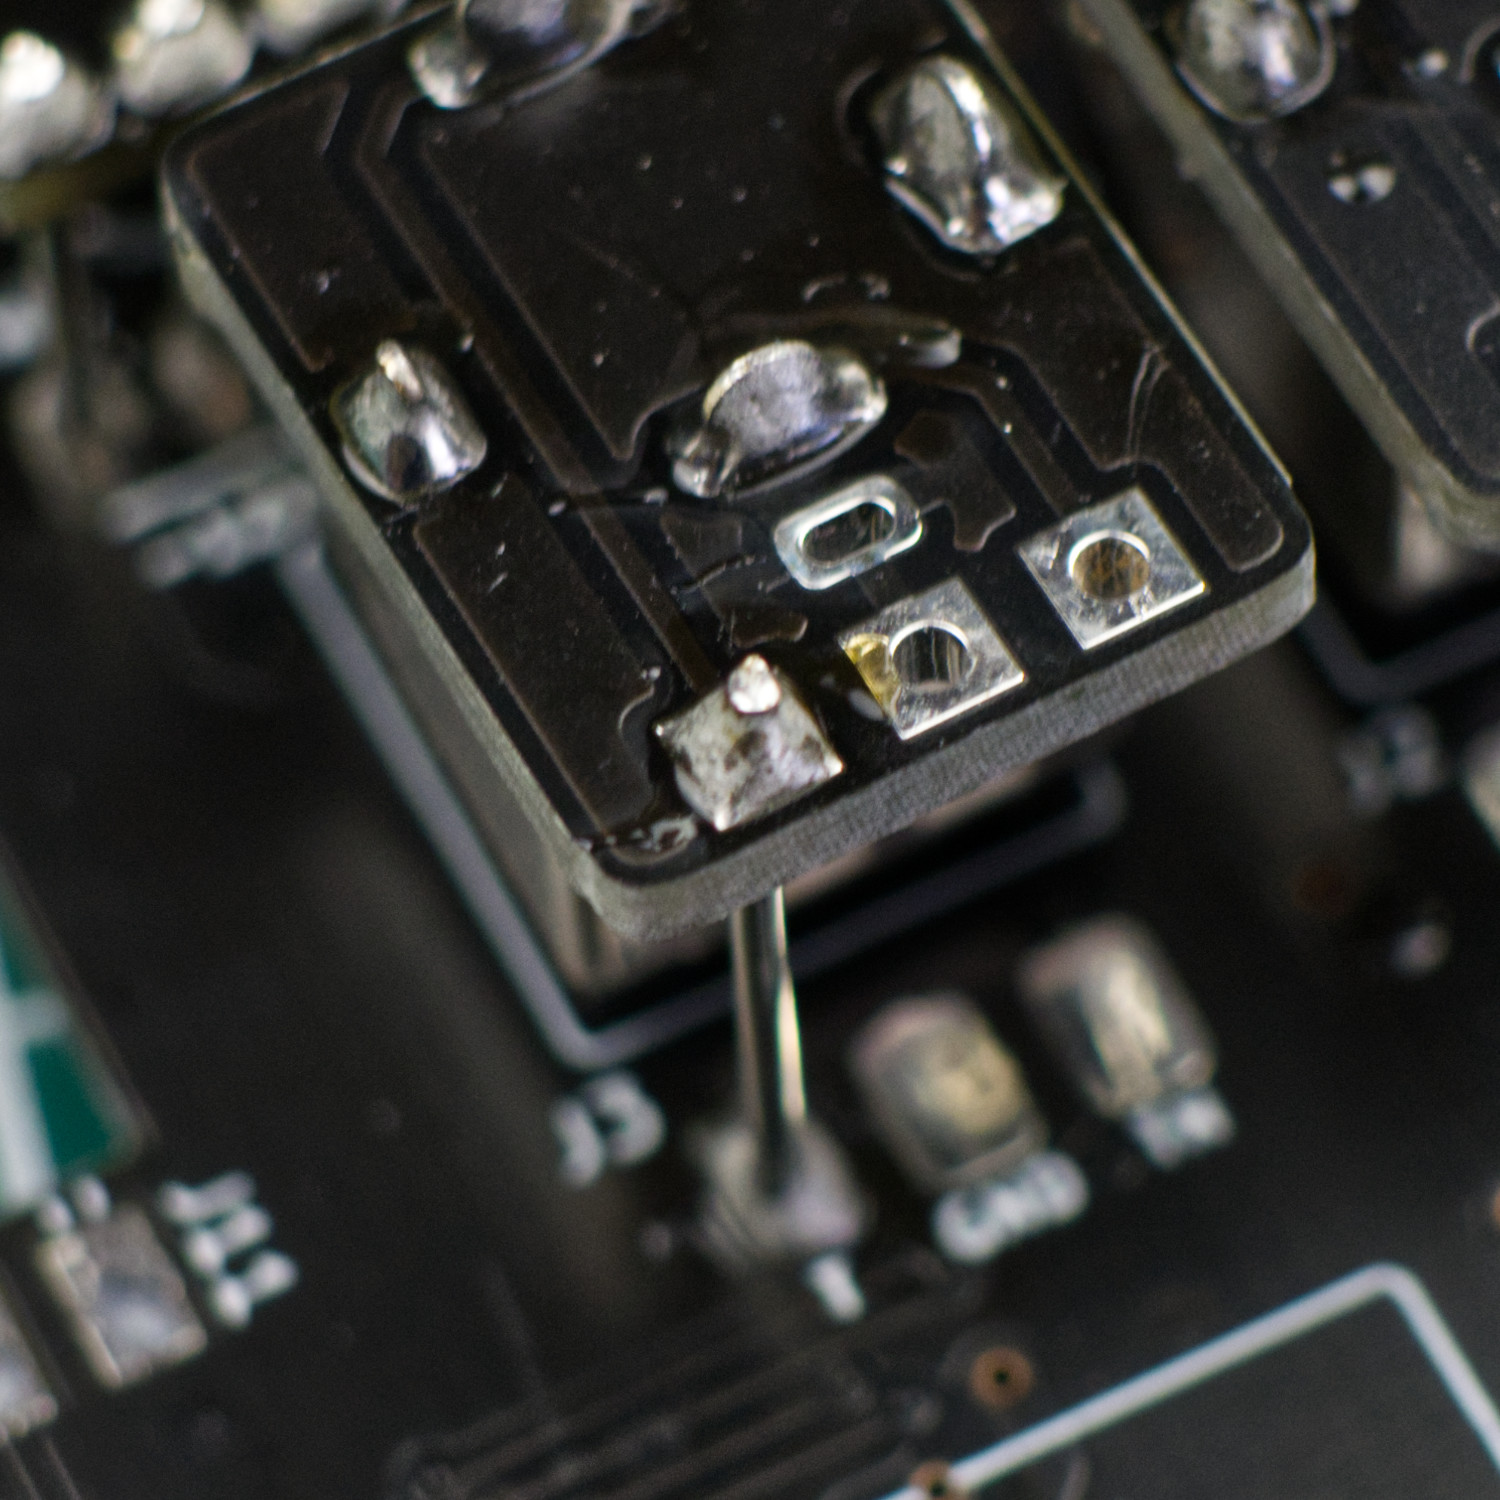
\includegraphics[width=46mm]{images/section_3-3_single_top.jpg}
    \hspace{2mm}
    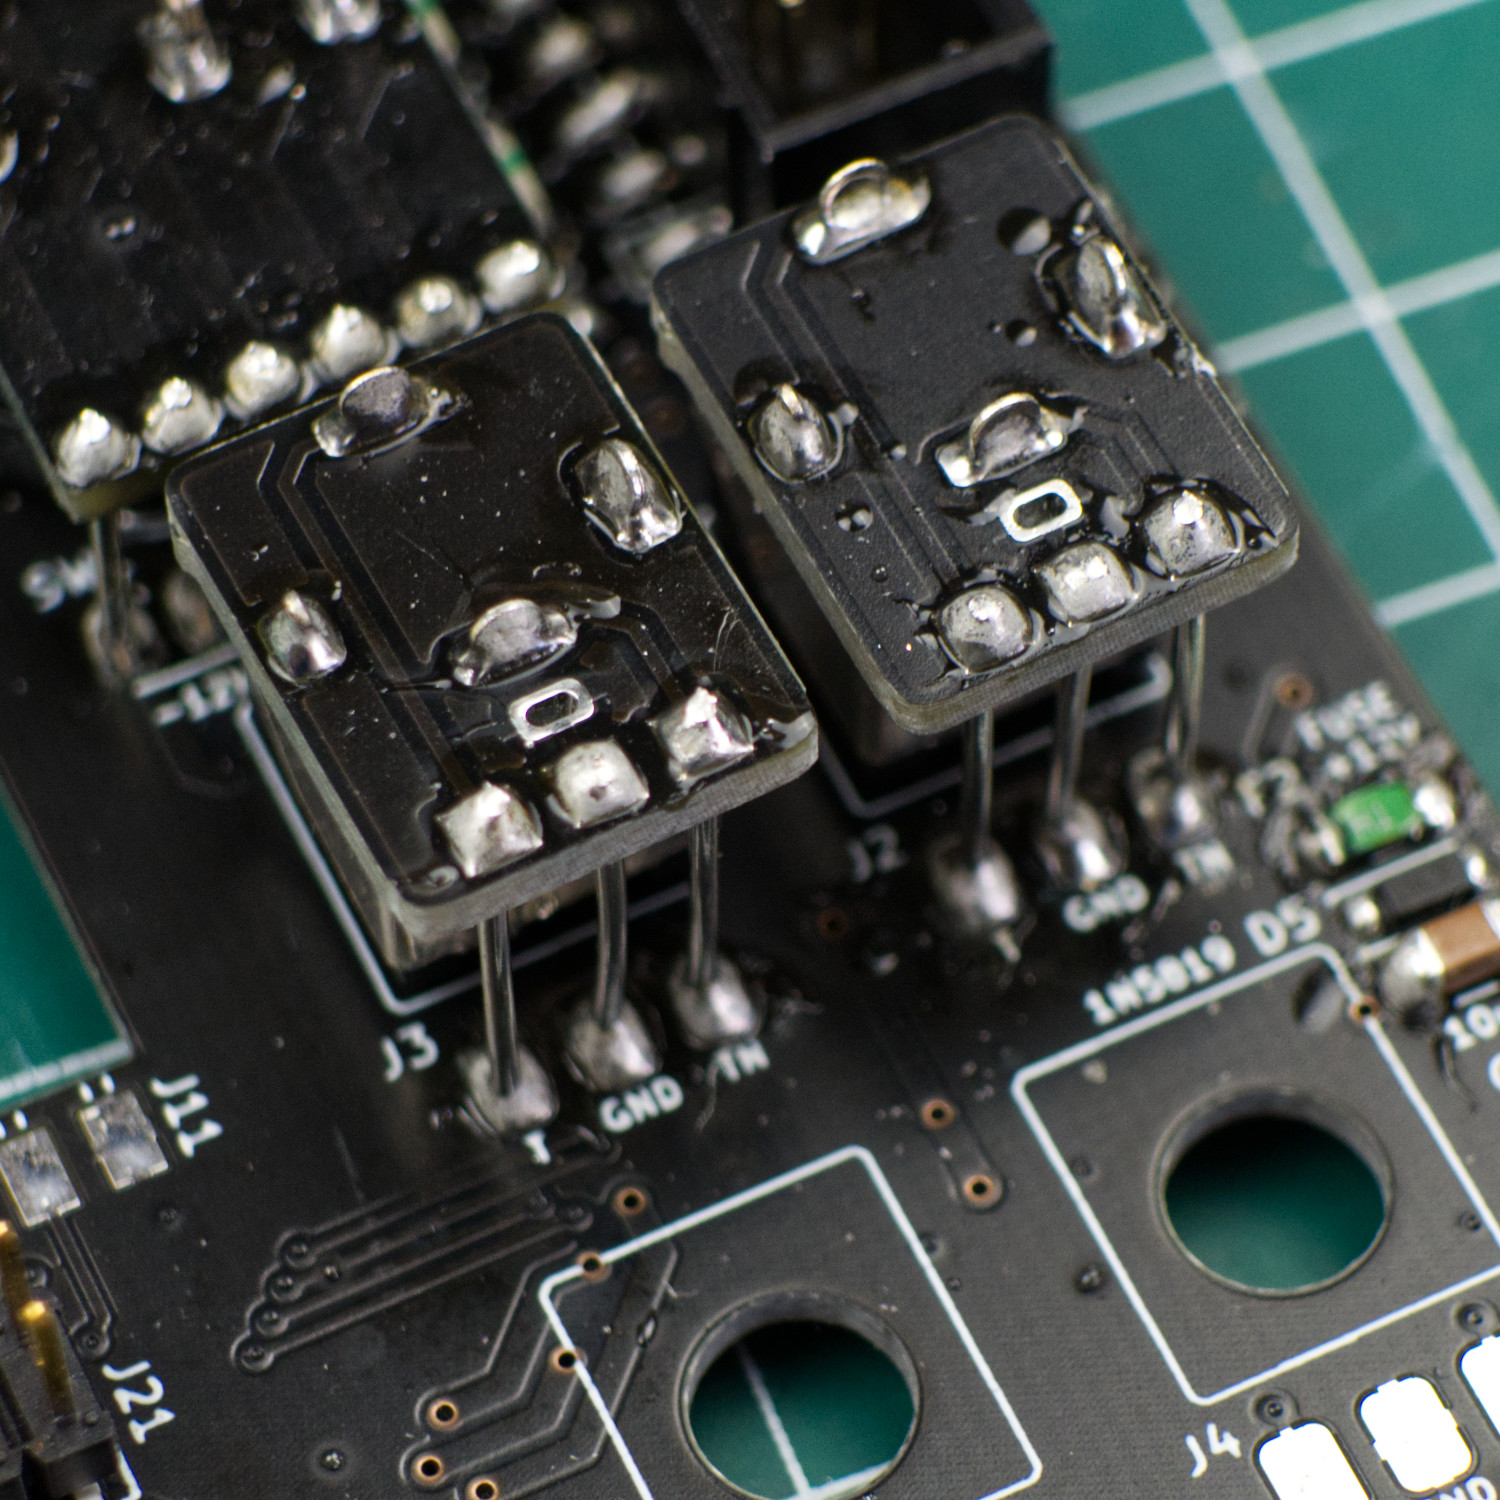
\includegraphics[width=46mm]{images/section_3-3_full.jpg}
\end{figure}

Use your multimeter in continuity mode to ensure you did not create any short-circuits. There
should not be any continuity between any of the wires.

\textbf{Repeat these steps for the remaining three rows of audio jacks.}

\subsection{Potentiometers}

\begin{center}
    \small
    \setlength\extrarowheight{8pt}
    \begin{tabularx}{\textwidth}{|c|c|c|X|l|}
        \hline\rowcolor{lightgray} & ID & Qty & Description & PCB Identifier\\
        \hline\checkbox{ja} & 27 & 4 & Potentiometer Knob & -\\
        \hline\checkbox{jb} & 28 & 4 & Potentiometer Nut & -\\
        \hline\checkbox{jc} & 29 & 4 & Potentiometer Spacer & -\\
        \hline\checkbox{jd} & 30 & 4 & 100k Potentiometer (linear) & RV1, RV2, RV3, RV4\\
        \hline\checkbox{je} & 31 & 4 & Potentiometer Dust Covers & -\\  % TODO: add instructions
        \hline
    \end{tabularx}
\end{center}

\subsubsection*{Tip:}
\vspace{-3mm}
\textbf{While not as critical as the audio jacks, this part is also easier to do if you follow the
steps for each potentiometer, one by one, from top to bottom.}
\vspace{5mm}

Attach the 3D printed spacers to the potentiometers. There is a little nubbin on one side, which
indexes into the PCB and helps to align the rotation of the potentiometer.

Next, use the included 3D printed tool to screw down the potentiometers to the PCB with the
hex nuts. Do not overtighten them, and make sure the potentiometer aligns with the pads on the
back of the PCB nicely.

Finally, bend down the solder lugs till they touch the PCB and solder them in place.
(If you do not have potentiometers with solder lugs but shorter pins, you can stack up some
solder to make them reach.)

\begin{figure}[H]
    \centering
    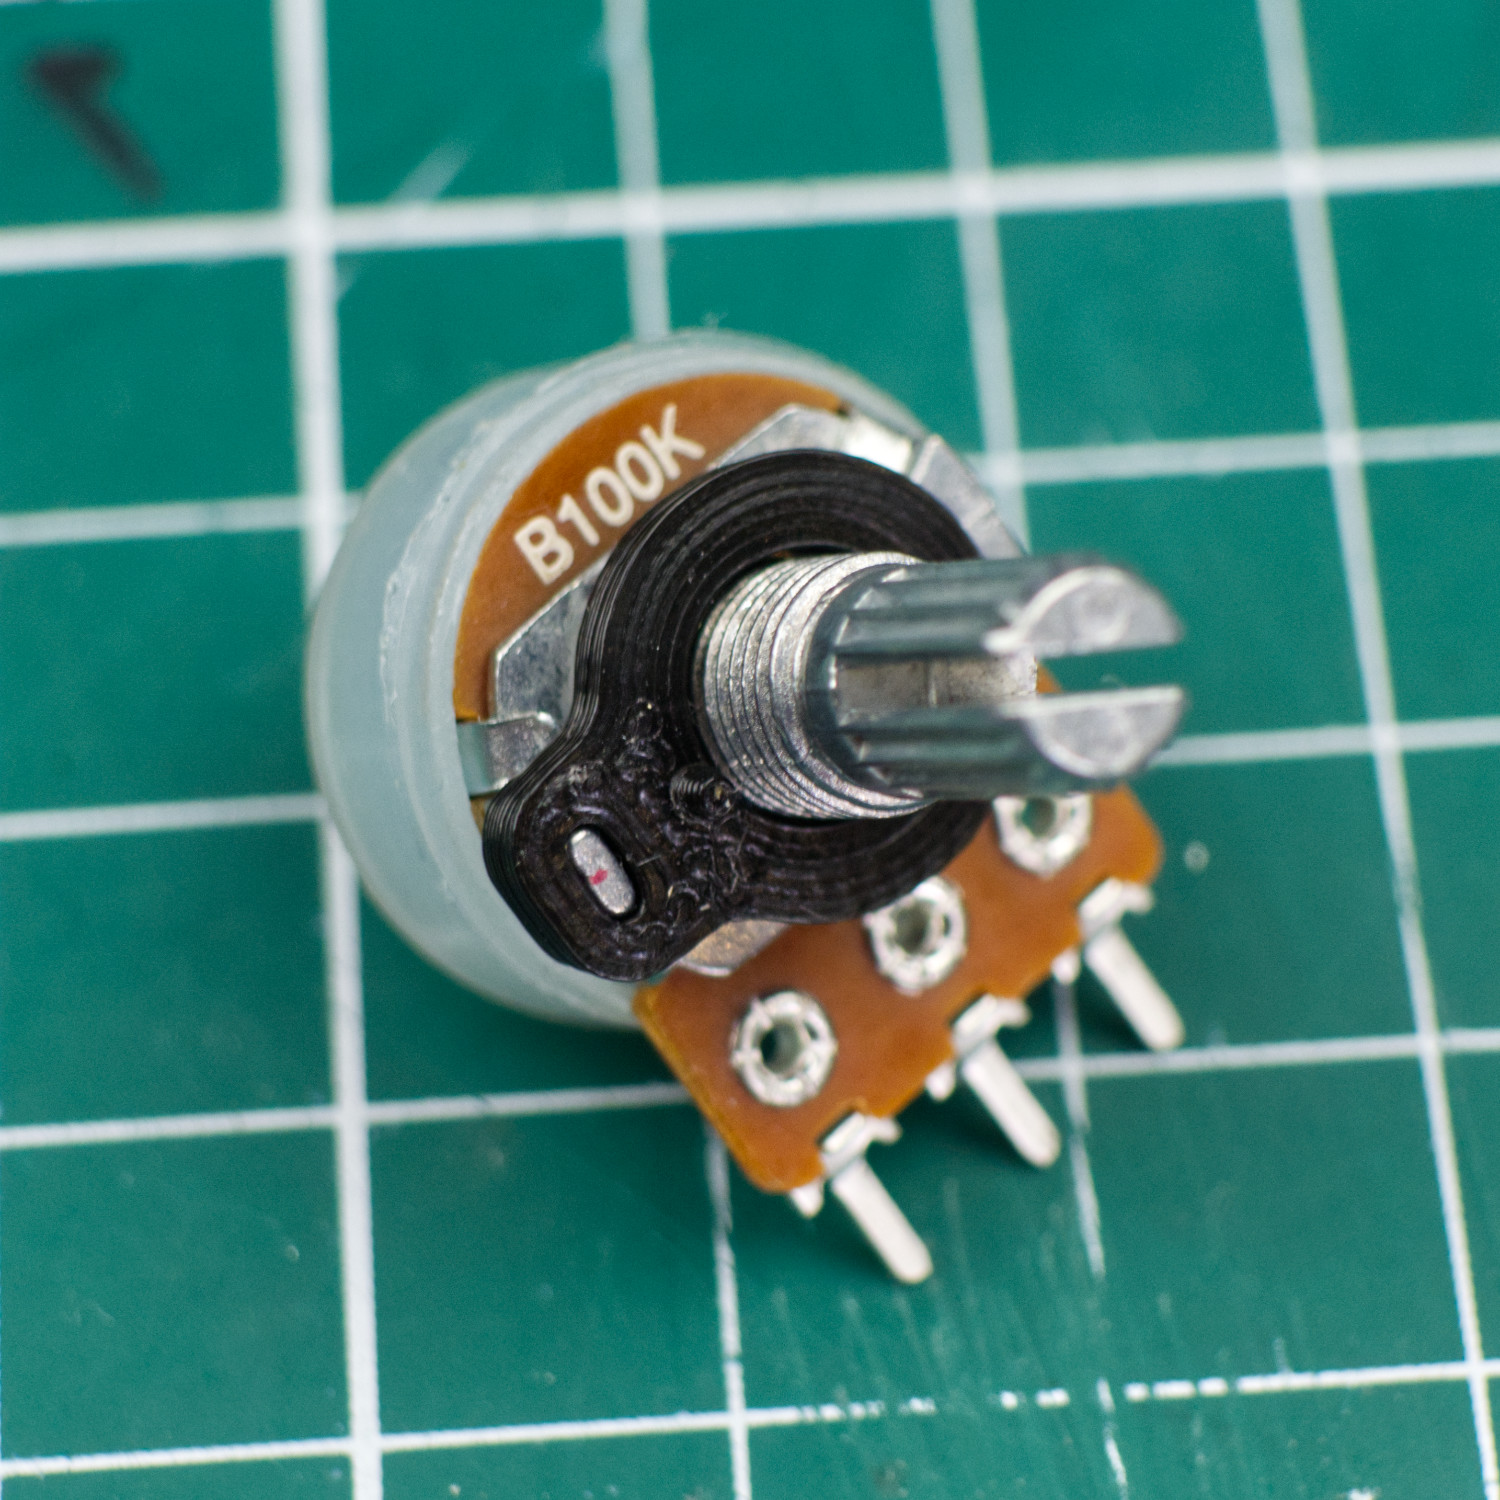
\includegraphics[width=46mm]{images/section_3-4_washer.jpg}
    \hspace{2mm}
    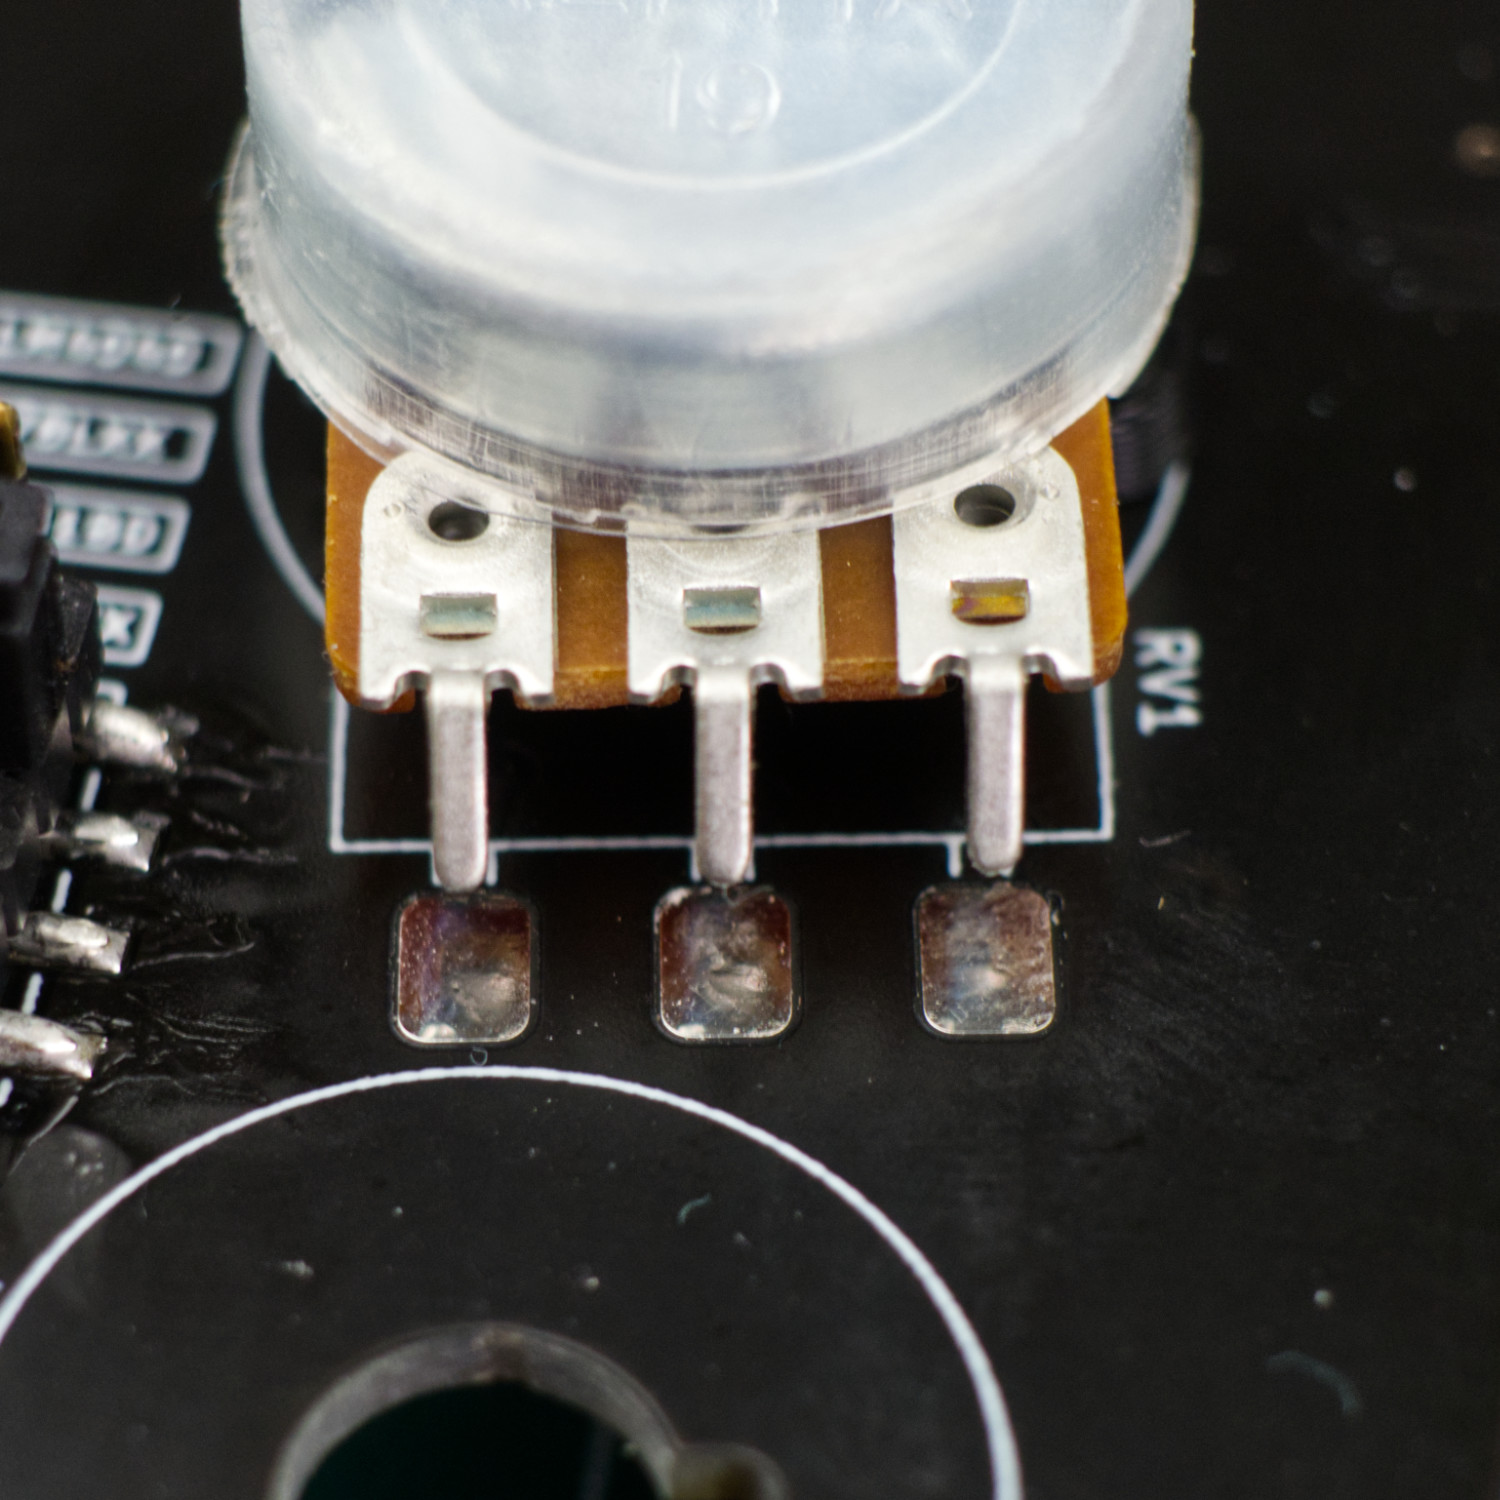
\includegraphics[width=46mm]{images/section_3-4_screwed.jpg}
    \hspace{2mm}
    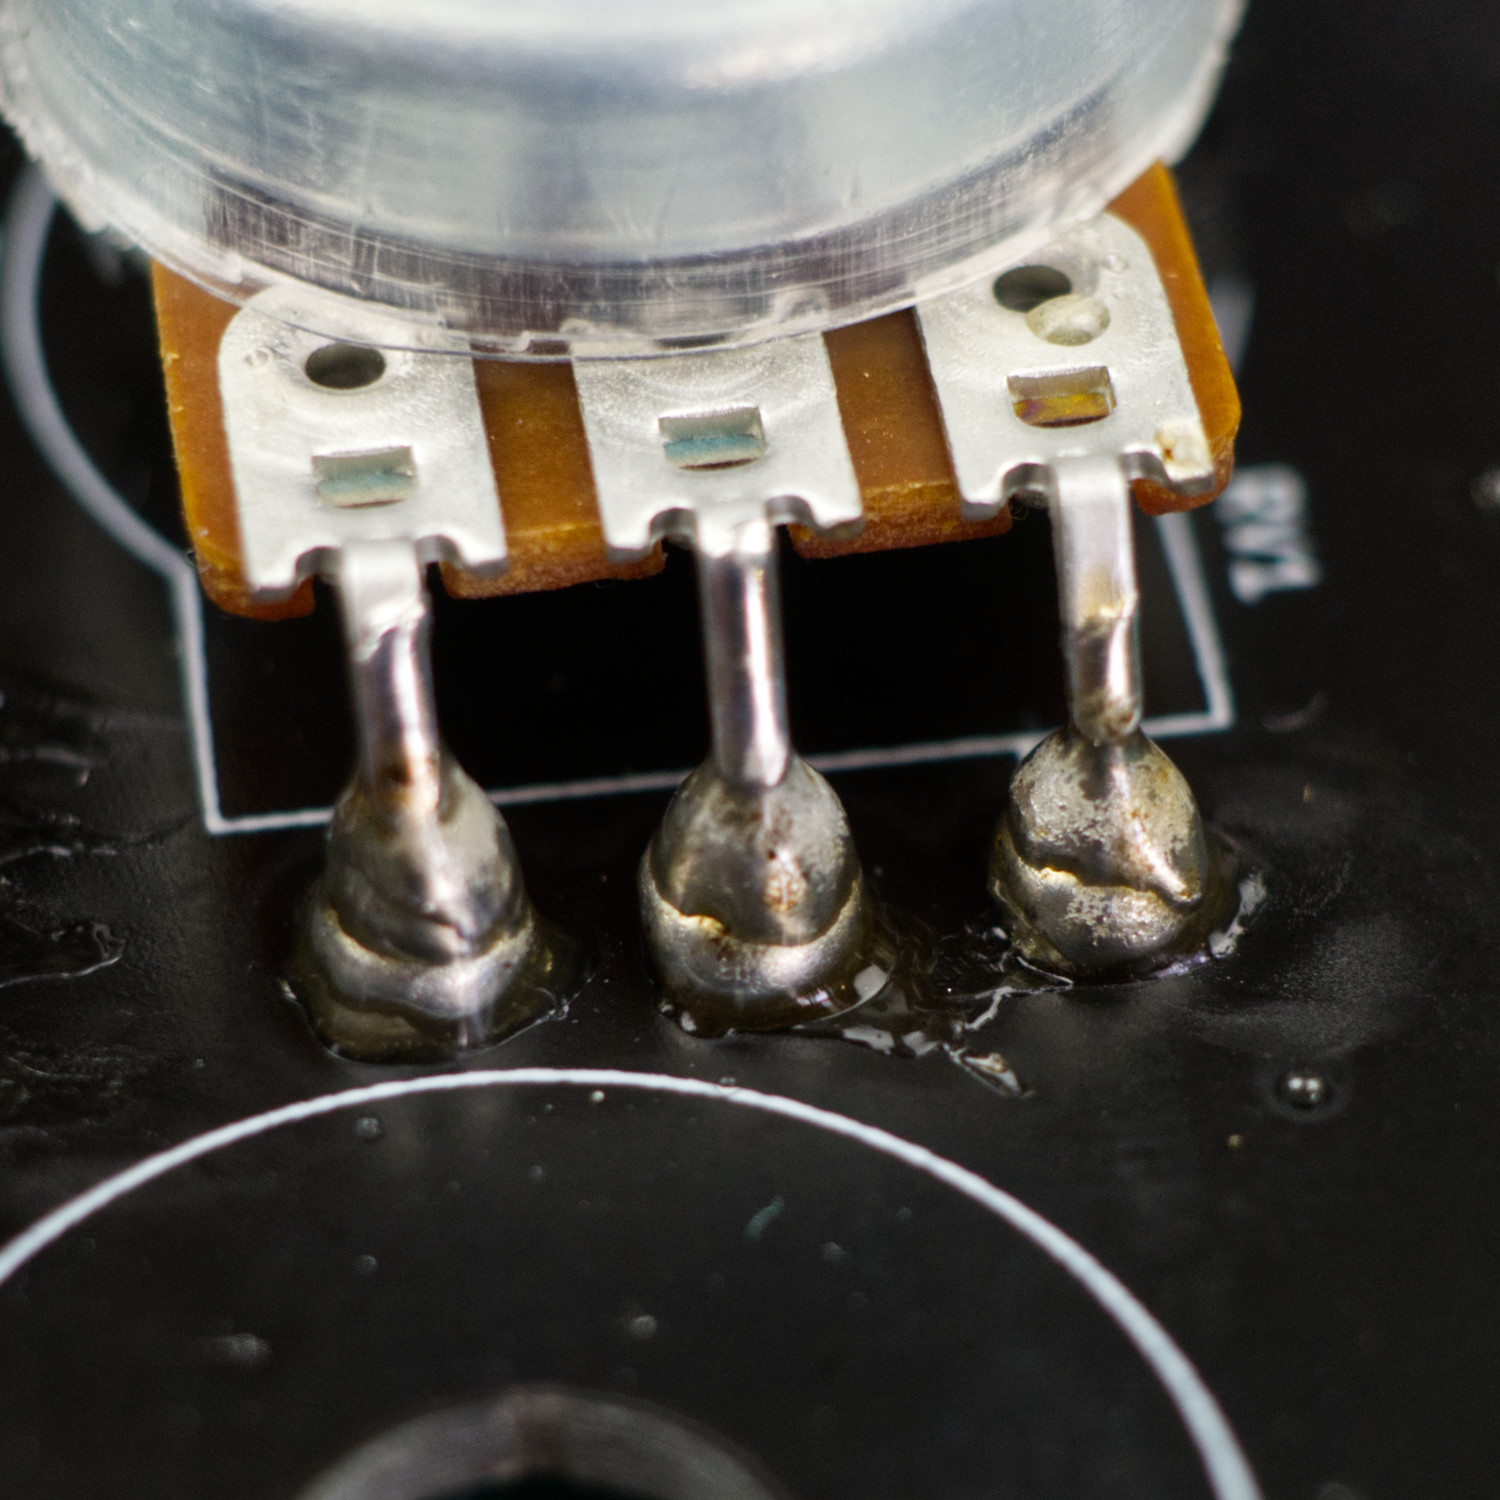
\includegraphics[width=46mm]{images/section_3-4_solder_stack.jpg}
\end{figure}

\pagebreak
\section{Breadboard}

\begin{figure}[H]
    \centering
    \begin{tikzpicture}
        \node[anchor=south west,inner sep=0] (image) at (0,0) {
            
\includegraphics[width=7cm]{images/placeholder.jpg}
        };
        \begin{scope}[x={(image.south east)},y={(image.north west)}]
        \end{scope}
    \end{tikzpicture}
    \hspace{2mm}
    
\includegraphics[width=7cm]{images/placeholder.jpg}
\end{figure}

\begin{center}
    \small
    \setlength\extrarowheight{8pt}
    \begin{tabularx}{\textwidth}{|c|c|c|X|}
        \hline\rowcolor{lightgray} & ID & Qty & Description\\
        \hline\checkbox{ka} & 29 & 4 & BB830 type breadboard\\
        \hline\checkbox{kb} & 30 & 5 & rubber feet\\
        \hline
    \end{tabularx}
\end{center}

Take the two breadboards and combine them by pushing them together using the nubbins and slots
on their sides.

Next, turn them around and start attaching the rubber feet to the bottom. Ideally, they should
be directly attached to the adhesive on the breadboards back. For this, use a
ruler to measure out five 20×20mm squares (one in the center and one in each corner).
Then use a utility knife to cut through the top cover of the adhesive and carefully peel it
off. Finally, peel off the cover film from the rubber feet and stick them onto the exposed
adhesive.

\begin{figure}[H]
    \centering
    
\includegraphics[width=46mm]{images/placeholder.jpg}
    \hspace{2mm}
    
\includegraphics[width=46mm]{images/placeholder.jpg}
    \hspace{2mm}
    
\includegraphics[width=46mm]{images/placeholder.jpg}
\end{figure}

\subsection{\smaller (optional) \enspace \larger Gluing}
\label{ssec:gluing}

TODO

\section*{Using Alternative Voltage References}

\subsection*{L78Lxx}

Any pin compatible, SOT-89 package Low-Dropout-Regulator can be used in place of the
default L78L05, as long as \enspace $V_D < 12V - V_O$ \enspace ($V_D$ and $V_O$ being the
regulators Dropout and Output-Voltage).

\subsection*{LM4040}

Any pin compatible, SOT-23-3 package LM4040 voltage reference can be used in place of the
default one, but the bias resistor will have to be adjusted.

\subsubsection*{Selecting the bias resistor}
\label{ssec:appendix_lm4040_selecting_bias_resistor}

The bias resistor connects between the LM4040s cathode and the supply voltage and sets the
available output/load current $I_L$, as well as its bias current $I_Z$.

The bias current is required to make the reference work and has to be within its operating
current range, which is \enspace $\sim \!\! 100\mu A < I_Z < 15mA $ \enspace
(depending on the exact reference used). We want to keep the bias current rather low to avoid
the reference heating up too much, while staying within the range and keeping some distance to
the extremes, so we target:

\[ I_Z = 1mA \tag*{$(a)$}\label{tag:a} \]

The load current is dependent on what is connected to the output of the reference. On the
spark inducer all voltage references are being buffered by two OpAmps:

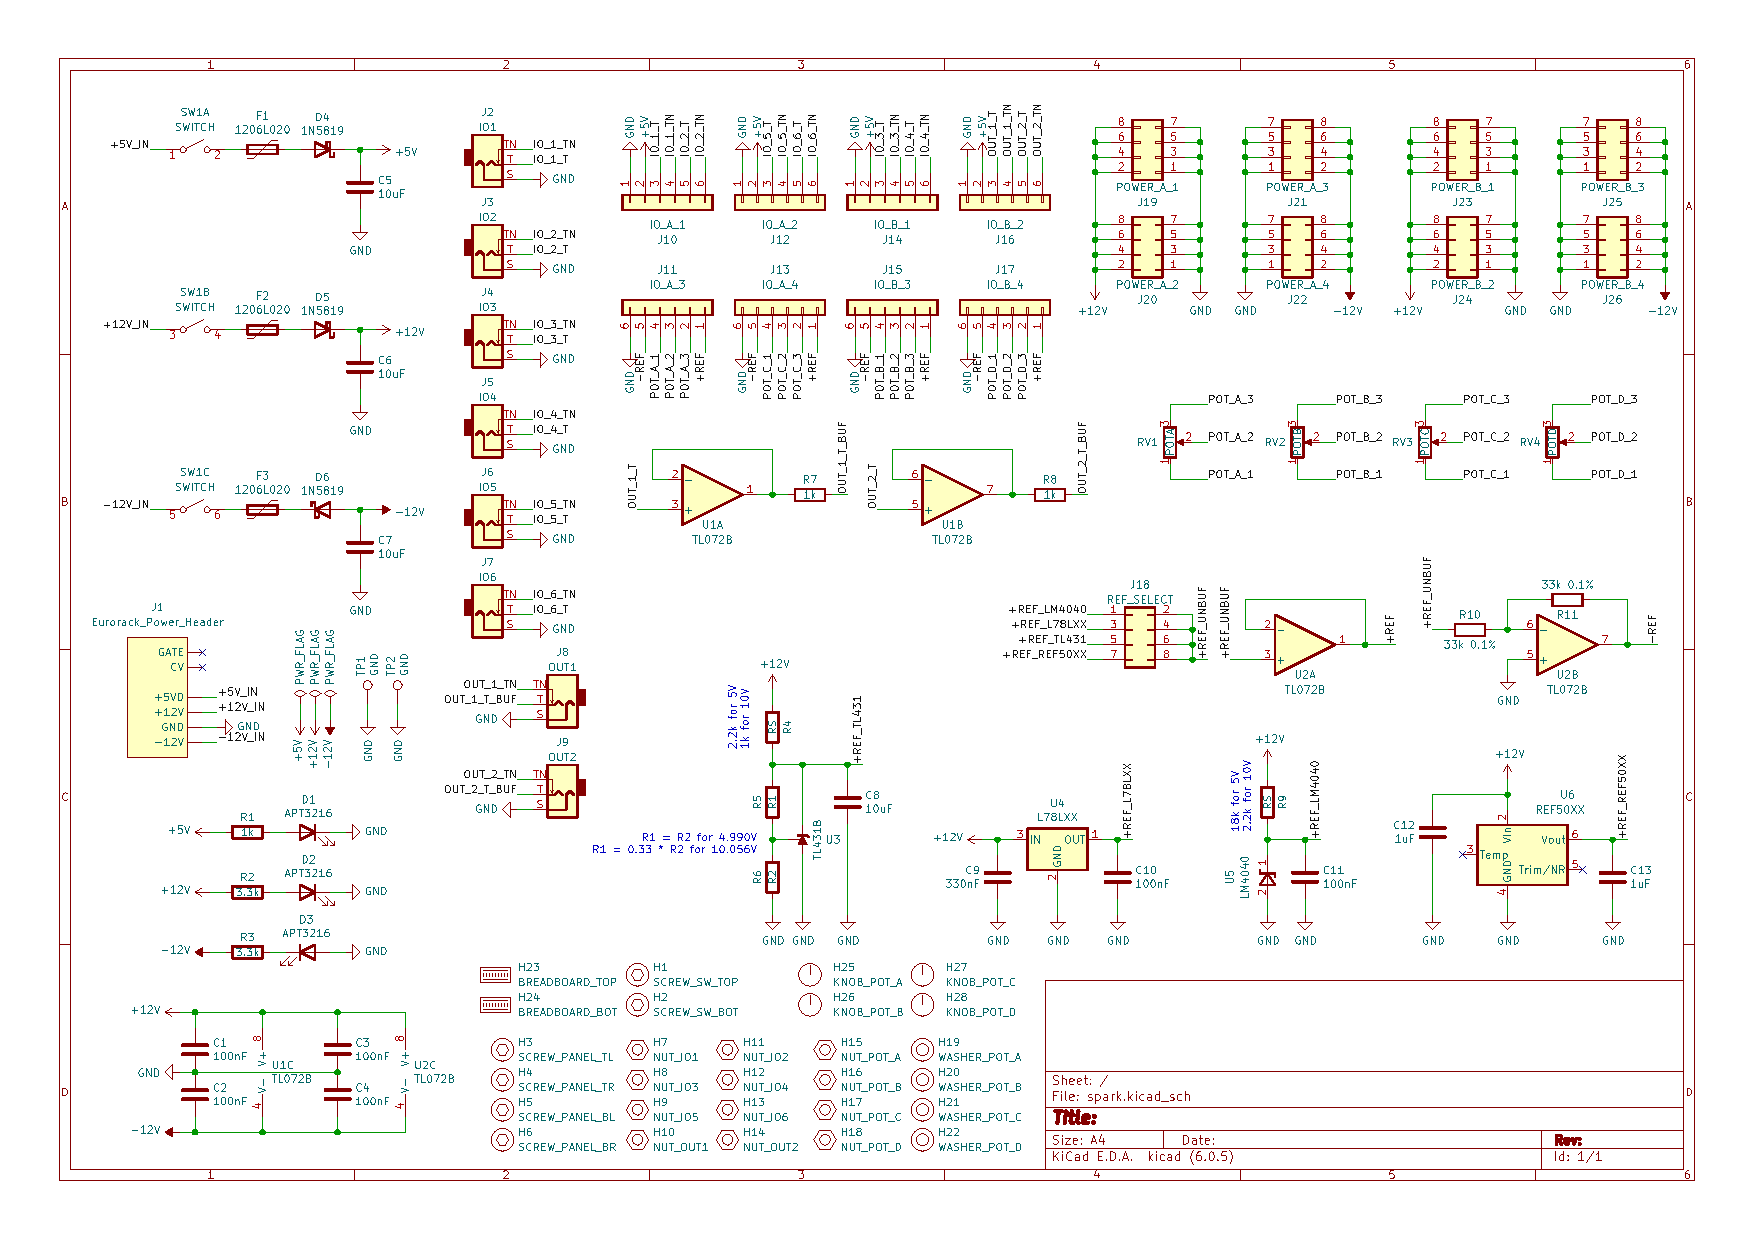
\includegraphics[width=\textwidth, trim = 16.7cm 8.9cm 1.5cm 9.1cm, clip=true]{pdf/schematic.pdf}

Thus, ignoring the input leakage currents of the OpAmps, the only load attached to the voltage
reference is R10, which is connected to a virtual ground, so the load current is constant and
equal to:

\[ I_L = \frac{V_Z}{33k\Omega} \tag*{$(b)$}\label{tag:b} \]

with $V_Z$ being the LM4040s Output-/Reference-Voltage.

To calculate the value of the bias resistor, the LM4040s datasheet specifies the equation:

\[ R_S = \frac{V_S - V_Z}{I_L + I_Z} \tag*{$(1)$} \]

So for our application, with \ref{tag:a}, \ref{tag:b} and $V_S = 12V$ we get:

\[ R_S = \frac{12V - V_Z}{\frac{V_Z}{33k \Omega} + 1mA} \tag*{$(2)$} \]

You can use this equation to calculate the approximate value for the bias resistor of the
spark inducers LM4040 voltage reference. Then select the closest E12 resistor value
(or the closest resistor value you have on hand) and confirm that the operating current is
\enspace $\sim 1mA$ \enspace with:

\[
    I_Z = \frac{V_S - V_Z}{R_{Selected}} - I_L \;\;\; \Rightarrow \;\;\;
    I_Z = \frac{12V - V_Z}{R_{Selected}} - \frac{V_Z}{33k \Omega} \tag*{$(3)$}
\]

\subsection*{TL431B}

TODO

\subsection*{REF50xx}

TODO

\pagebreak
\section*{Board View}
\includegraphics[angle=90, origin=c, width=\textwidth]{pdf/back_silkscreen.pdf}

\pagebreak
\section*{Schematic}
\includegraphics[angle=90, origin=c, width=\textwidth]{pdf/schematic.pdf}

\pagebreak
\section*{Bill of Materials}
\begin{center}{
    \scriptsize
    \ibmplex
    \setlength\extrarowheight{-5pt}
    \csvreader[
        separator = semicolon,
        respect all,
        head to column names,
        tabular = l>{\raggedright}p{2.65cm}>{\raggedright}p{3.8cm}ll,
        table head = \hline \\ Qty & Reference & Value & Part Number & Note \\ \hline,
        table foot = \hline,
    ]{bom.csv}{}{
        \\ \Quantity\ & \Reference & \Value & \PartNumber & \SubstituteCriteria
    }
}\end{center}

\end{document}
